\clearpage
\thispagestyle{empty}
\null
\newpage

\cleardoublepage
\phantomsection
% \pdfbookmark[1]{La méthode MAMAD}{La méthode MAMAD}
\markboth{\spacedlowsmallcaps{La méthode MAMAD}}{\spacedlowsmallcaps{La méthode MAMAD}}
\part{La méthode MAMAD}
\label{part:methode}

\clearpage
\thispagestyle{empty}
\null
\newpage

% todo : Initialement, dans la partie I, notre problème était un problème de conception logiciel d'un \acn{SMA} de Cyberdéfense capable d'assurer la Cyberdéfense de façon optimale compte tenu des contraintes dynamique de l'environnement et des concepteur. Nous avons formalisé le fait que pour répondre à cette question de recherche globale, il faut répondre simultanément à 6 critères (Autonomie - C1, Performance - C2, Adaptation - C3, Contrôle - C4, Explicabilité - C5, Robustesse - C6). Nous avons donc poursuivi une première revue de littérature qui nous a permis de comprendre qu'assez peu de travaux s’intéressent à une approche multi-agent pour la Cyberdéfense et que les travaux qui couvrent le plus de critères sont à chercher du côté de l'approche connexioniste qui favorise la performance et l'adaptation là où l'approche purement symbolique favorise l'explicabilité et le controle. Fort de ce constat, nous avons proposé de voir la question de recherche globale au travers le prisme d'un problème d'optimisation sous contraintes où la politique conjointe est à optimiser pour maximiser une récompense qui encode le succès dans l'atteinte d'un objectif de Cyberdéfense (ou un conglomérat d'objectifs) et où les contraintes sont formalisées comme des spécifications organisationnelles. A partir de cette formalisation, la complexité de la question de recherche globale apparait abordable au travers de 4 activités : Modélisation, Entrainement, Analyse et Transfert. On sait pour chaque activité les données en entrée, les données en sortie attendues et donc aussi les objectifs de chaque activité.
% A partir de cette vision, la partie \acn{II} présente les travaux qui couvrent les objectifs pour chaque activité, permettant ainsi de savoir quels sont les domaines/sous-domaines ou travaux qui semble le plus adaptés (ou qui nécéssitent le moins de contributions supplémentaires) pour atteindre les objectifs de chaque activités. Compte tenu des travaux identifiés comme les plus prometteurs, on en déduit donc les verrous qui restent encore à combler par de nouvelles contributions pour atteindre les objectifs de chaque activités.
% La partie \acn{III}, présente la méthode qui orchestre les 4 activités et explique dans chacune des activités comment nous avons combler les verrous par de nouvelles contributions. Dans cette partie, une présentation générale de la méthode qui orchestre les 4 activités est d'abord donnée. Ensuite, nous détaillons chaque activité en rappellant rapidement les objectifs et chacun des verrous associés et pour chacun nous détaillons notre contribution en les justifiant. Une fois ceci fait, nous donnons une représentation alogrithmique de l'activité qui sert de support pour détailler de façon formelle l'activité en explicitant chacun des éléments formels (ensemble, élément d'un ensemble, relation...). A la fin de l'activité, on fait une sorte de bilan en expliquant ce qu'on pense qui sera couvert en termes d'objectifs attendus, ce qui l'est moyennement et pourquoi et ce qui n'est pas du tout couvert.
% La partie \acn{IV} concerne la validation expérimentale de la méthode par la mise en application de cette méthode au travers de trois cas d'études non-orientés Cyberdéfense et de trois cas d'études orientés Cyberdéfense. L'objectif est de vérifier que les 6 critères (Autonomie - C1, Performance - C2, Adaptation - C3, Contrôle - C4, Explicabilité - C5) sont bien couverts. Pour cela, on applique une grille d'évaluation qui associe chaque critères à un ensemble de métriques mesurables et qui peuvent être analysé pour voir si le critère est couvert ou pas. Comme la grille de lecture est commune aux 6 environnements, on peut donc vérifier de manière plus consistante et générique si la méthode permet bien de couvrir les 6 critères. La partie finit donc avec une analyse globale de si la méthode couvre bien les 6 critères posés initialement.

% \acn{TODO}:
%  - Globalement, harmoniser le vocabulaire
%  - Globalement, introduire correctement les termes techniques/théoriques comme "Adéquation organisationel", "\acn{RNN}", "\acn{VAE}", "\acn{LSTM}", "World Models" notamment pour permettre à un lecteur non familier avec le \acn{ML} ou l'\acn{IA} en général de comprendre.
%  - Dans les chapitres concernant les activités de "Modélisation", "Entrainement", "Analyse" et "Transfert", il faudra veiller à bien expliciter les objectifs de chacune des activités, les hypothèses qui délimitent notre espace de recherche dans la littérature, les travaux les plus susceptibles d'atteindre les objectifs de l'activité (par exemple : le Constrained-\acn{RL}, Shielding...) et les verrous associés restants à relever (par exemple : le manque de moyen permettant de guider l'apprentissage avec un modèle organisationel) par de nouvelles contributions. Ensuite, on présente ces différentes contributions (par exemple : le framework MOISE+MARL). Ensuite, on peut présenter l'activité sous la forme d'un algorithme qui articule les travaux identifiés et/ou contributions pour répondre aux objectifs de l'activité. Il faudra veiller à bien expliciter en détail cet algorithme (en référençant chacun des éléments formel de l'algorithme) pour donner une description la plus complète possible de l'activité. Pour finir, on doit dire en quoi nous pensons que cette implémentation de l'activité permet bien de répondre aux objectifs de l'activité ou pas. Plus loin, on peut même dire si nous pensons que les critères associé à une activité sont bien couvertes avec cette implémentation actuelle de l'activité.

\chapter*{Introduction}
\addcontentsline{toc}{chapter}{\textbf{Introduction}}

\noindent

La partie précédente a mis en lumière les lacunes actuelles dans l'intégration des modèles organisationnels au sein des approches d'apprentissage multi-agent, tant du point de vue du contrôle, de l'explicabilité que de l'automatisation de la conception. Elle a également mis en lumière les lacunes dans la modélisation de l'environnement et son intégration dans le processus d’entraînement notamment sur le manque de cadre permettant d'assurer la cohérence entre l'environnement simulé et réel.

\medskip

\noindent
Cette troisième partie présente notre proposition pour répondre à ces lacunes~: la méthode \acn{MAMAD}. Cette méthode repose sur la prémisse que la conception d'un \acn{SMA} peut être abordée par le prisme d'un problème d'optimisation sous contraintes. La méthode est construite autour de cette vision et s'organise donc autour de quatre activités~:

\begin{enumerate}
    \item \textbf{Modélisation}~: modéliser l'environnement réel en un environnement simulé ainsi que les contraintes de conceptions en spécifications organisationnelles~;
    \item \textbf{Apprentissage}~: entraîner les agents dans cet environnement simulé en tenant compte de spécifications organisationnelles comme des rôles durant l'apprentissage~;
    \item \textbf{Analyse}~: extraire des spécifications structurelles et fonctionnelles émergentes à partir des trajectoires des agents entrainés~;
    \item \textbf{Transfert}~: mettre à jour régulièrement les politiques des agents déployés dans l'environnement réel à partir des politiques des agents entrainés en simulation et éventuellement mettre à jour ou améliorer l'environnement simulé.
\end{enumerate}

\noindent
Ces quatres activités peuvent être vues comme exécutées de façon itérative pour produire des \acplu{SMA} adaptés à leur environnement, alignés sur des contraintes organisationnelles, explicables et robustes.

\medskip

\noindent
Le \autoref{chap:mamad_global} donne une description globale de la méthode concernant les processus proposés. Les quatre chapitres restants détaillent chacune des étapes de cette méthode~:
Le \autoref{chap:modelling} présente l'activité de modélisation.
Le \autoref{chap:training} présente l'activité d'apprentissage contraint par des spécifications organisationnelles.
Le \autoref{chap:analyzing} présente une méthode permettant d'analyser des trajectoires pour inférer des structures organisationnelles émergentes.
Le \autoref{chap:transferring} décrit l'activité de transfert.
La \autoref{fig:organisation_manuscrit_partie_3} illustre cette organisation de cette partie.

La méthode \acn{MAMAD} ambitionne de réunir les forces des approches symboliques et apprenantes pour une conception de \acn{SMA} à la fois structurée, autonome et explicable.

\begin{figure}[h!]
    \centering
    \resizebox{0.8\linewidth}{!}{%
        \begin{tikzpicture}[
        chapter/.style={draw, fill=blue!10, thick, minimum width=9cm, minimum height=1.2cm, text centered, font=\bfseries},
        section/.style={draw, fill=blue!5, thick, minimum width=8cm, minimum height=1cm, text centered, font=\small},
        arrow/.style={-Latex, thick},
        node distance=0.4cm,
        annotated/.style={above,font=\small\itshape, inner sep=1pt, yshift=0.8cm, xshift=-8cm}
    ]

    % Chapitre 6 : MAMAD comme réponse
    \node[chapter] (ch6) {\parbox{15cm}{\centering Chapitre 6 : La méthode MAMAD}};
    \node[section, below=1cm of ch6, xshift=-2cm] (ch6s1) {Principes et boucle itérative fermée};
    \node[section, below=1cm of ch6s1] (ch6s2) {L'architecture générale de la méthode MAMAD};

    \draw[arrow] ($ (ch6.south) + (4.0,0) $) -- ++(0,0) |- (ch6s1.east) node[annotated] {Définit les fondements et la structure en boucle fermée de la méthode MAMAD};
    \draw[arrow] ($ (ch6.south) + (4.0,0) $) -- ++(0,0) |- (ch6s2.east) node[annotated] {Présente les composants logiciels et l'enchaînement des activités de la méthode};

    % Chapitre 7 : Activité 1 — Modélisation
    \node[chapter, below=1cm of ch6s2, xshift=2cm] (ch7) {Chapitre 7 : Modéliser l'environnement en simulation};
    \node[section, below=1cm of ch7, xshift=-2cm] (ch7s1) {Reconstruction partielle de l'environnement};
    \node[section, below=1cm of ch7s1] (ch7s2) {Apprentissage de la dynamique observable};
    \node[section, below=1cm of ch7s2] (ch7s3) {Modélisation des exigences de conception et de l'objectif};

    \draw[arrow] ($ (ch7.south) + (4.0,0) $) -- ++(0,0) |- (ch7s1.east) node[annotated] {Reconstituer les éléments essentiels de l'environnement réel pour générer une base simulée};
    \draw[arrow] ($ (ch7.south) + (4.0,0) $) -- ++(0,0) |- (ch7s2.east) node[annotated] {Apprendre la dynamique partiellement observable à partir de données collectées ou simulées};
    \draw[arrow] ($ (ch7.south) + (4.0,0) $) -- ++(0,0) |- (ch7s3.east) node[annotated] {Formaliser les objectifs et contraintes pour guider l'apprentissage à venir};

    \draw[arrow] ($ (ch6.south) + (4.5,0) $) -- ($ (ch7.north) + (4.5,0) $) node[annotated, yshift=-0.5cm] {La méthode débute par la création d'un environnement simulé réaliste intégrant objectifs et contraintes};

    % Chapitre 8 : Activité 2 — Apprentissage guidé
    \node[chapter, below=1cm of ch7s3, xshift=2cm] (ch8) {Chapitre 8 : Entraînement des politiques sous contraintes};
    \node[section, below=1cm of ch8, xshift=-2cm] (ch8s1) {Cadres Markoviens utilisés};
    \node[section, below=1cm of ch8s1] (ch8s2) {Guider et contraindre l'apprentissage};
    \node[section, below=1cm of ch8s2] (ch8s3) {Une politique conjointe composite pour l'incertitude};

    \draw[arrow] ($ (ch8.south) + (4.0,0) $) -- ++(0,0) |- (ch8s1.east) node[annotated] {Définit les cadres formels (Dec-POMDP) utilisés pour l'apprentissage multi-agent};
    \draw[arrow] ($ (ch8.south) + (4.0,0) $) -- ++(0,0) |- (ch8s2.east) node[annotated] {Explique les mécanismes de guidage et de contrainte injectés durant l'entraînement};
    \draw[arrow] ($ (ch8.south) + (4.0,0) $) -- ++(0,0) |- (ch8s3.east) node[annotated] {Décrit une stratégie robuste face à l'incertitude via une politique composite};

    \draw[arrow] ($ (ch7.south) + (4.5,0) $) -- ($ (ch8.north) + (4.5,0) $) node[annotated, yshift=-0.5cm] {Une fois l'environnement modélisé, les agents peuvent être entraînés à agir sous contraintes organisationnelles};

    % Chapitre 9 : Activité 3 — Analyse
    \node[chapter, below=1cm of ch8s3, xshift=2cm] (ch9) {Chapitre 9 : Analyser les comportements émergents};
    \node[section, below=1cm of ch9, xshift=-2cm] (ch9s1) {Inférer les rôles et objectifs à partir des trajectoires};
    \node[section, below=1cm of ch9s1] (ch9s2) {Mesurer l'adéquation organisationnelle};

    \draw[arrow] ($ (ch9.south) + (4.0,0) $) -- ++(0,0) |- (ch9s1.east) node[annotated] {Analyse les trajectoires pour identifier rôles implicites et objectifs suivis par les agents};
    \draw[arrow] ($ (ch9.south) + (4.0,0) $) -- ++(0,0) |- (ch9s2.east) node[annotated] {Mesure la cohérence entre l'organisation visée et les comportements observés};

    \draw[arrow] ($ (ch8.south) + (4.5,0) $) -- ($ (ch9.north) + (4.5,0) $) node[annotated, yshift=-0.5cm] {Les politiques apprises sont ensuite analysées pour révéler les structures organisationnelles émergentes};

    % Chapitre 10 : Activité 4 — Transfert
    \node[chapter, below=1cm of ch9s2, xshift=2cm] (ch10) {Chapitre 10 : Transférer et superviser en environnement réel};
    \node[section, below=1cm of ch10, xshift=-2cm] (ch10s1) {Les différents modes de transfert opérationnel};
    \node[section, below=1cm of ch10s1] (ch10s2) {Bouclage entre environnement réel et simulation};

    \draw[arrow] ($ (ch10.south) + (4.0,0) $) -- ++(0,0) |- (ch10s1.east) node[annotated] {Décrit les modalités possibles de transfert des politiques vers le monde réel};
    \draw[arrow] ($ (ch10.south) + (4.0,0) $) -- ++(0,0) |- (ch10s2.east) node[annotated] {Précise comment maintenir une boucle entre terrain et simulation pour améliorer les performances};

    \draw[arrow] ($ (ch9.south) + (4.5,0) $) -- ($ (ch10.north) + (4.5,0) $) node[annotated, yshift=-0.5cm] {Les politiques validées peuvent être transférées dans l'environnement réel avec supervision adaptative};

    \draw[arrow] ($ (ch6.south) + (6.5,0) $) -- ++(0,0) |- (ch7.east);
    \draw[arrow] ($ (ch6.south) + (6.5,0) $) -- ++(0,0) |- (ch8.east);
    \draw[arrow] ($ (ch6.south) + (6.5,0) $) -- ++(0,0) |- (ch9.east);
    \draw[arrow] ($ (ch6.south) + (6.5,0) $) -- ++(0,0) |- (ch10.east);

\end{tikzpicture}

    }
    \caption{Structure de la Partie III~: La méthode MAMAD}
    \label{fig:organisation_manuscrit_partie_3}
\end{figure}



\clearpage
\thispagestyle{empty}
\null
\newpage

\chapter{Présentation globale de la méthode}
\label{chap:mamad_global}

La méthode \acn{MAMAD}~\footnotemark[2] repose sur quatre grandes activités~: (1) la modélisation de l'environnement, de l'objectif global et des contraintes organisationnelles, (2) l'apprentissage des politiques à l'aide de divers algorithmes \acn{MARL}, (3) l'analyse des comportements et l'inférence des spécifications organisationnelles à l'aide d'une méthode proposée, et (4) le maintien de la cohérence entre l'environnement simulé et l'environnement réel en déployant les politiques entraînées et en mettant à jour la simulation. Cette approche guide le processus d'apprentissage des agents tout en imposant des contraintes organisationnelles strictes, garantissant ainsi l'efficacité des politiques apprises.

Le cycle de vie d'un \acn{SMA} conçu avec \acn{MAMAD} est illustré en \autoref{fig:cycle}. Il commence par la modélisation de l'environnement, réalisée à partir d'un ensemble suffisant de trajectoires réelles (issues d'agents déjà transférés ou de toute autre source disponible), ainsi que la définition de l'objectif global et des contraintes de conception sous forme de rôles et d'objectifs. Ensuite, les agents sont entraînés dans cet environnement simulé à l'aide de techniques d'apprentissage par renforcement multi-agent (\acn{MARL}). Une fois l'entraînement terminé, une analyse post-entraînement permet d'extraire les rôles et objectifs émergents des agents, ce qui conduit à l'amélioration des spécifications organisationnelles appliquées. Enfin, après validation, les politiques apprises sont déployées pour contrôler les actionneurs de l'environnement, générant ainsi de nouvelles traces qui serviront à affiner la modélisation lors des itérations suivantes.

\begin{figure}[h!]
    \centering
    


\tikzset{every picture/.style={line width=0.75pt}} %set default line width to 0.75pt        

\begin{tikzpicture}[x=0.75pt,y=0.75pt,yscale=-1,xscale=1]
%uncomment if require: \path (0,3307); %set diagram left start at 0, and has height of 3307

%Shape: Smiley Face [id:dp29065495216725257] 
\draw  [line width=1.5]  (85.38,2800.11) .. controls (85.38,2797.7) and (87.16,2795.75) .. (89.36,2795.75) .. controls (91.55,2795.75) and (93.34,2797.7) .. (93.34,2800.11) .. controls (93.34,2802.52) and (91.55,2804.48) .. (89.36,2804.48) .. controls (87.16,2804.48) and (85.38,2802.52) .. (85.38,2800.11) -- cycle ; \draw  [line width=1.5]  (87.61,2798.63) .. controls (87.61,2798.39) and (87.78,2798.19) .. (88,2798.19) .. controls (88.22,2798.19) and (88.4,2798.39) .. (88.4,2798.63) .. controls (88.4,2798.87) and (88.22,2799.07) .. (88,2799.07) .. controls (87.78,2799.07) and (87.61,2798.87) .. (87.61,2798.63) -- cycle ; \draw  [line width=1.5]  (90.31,2798.63) .. controls (90.31,2798.39) and (90.49,2798.19) .. (90.71,2798.19) .. controls (90.93,2798.19) and (91.11,2798.39) .. (91.11,2798.63) .. controls (91.11,2798.87) and (90.93,2799.07) .. (90.71,2799.07) .. controls (90.49,2799.07) and (90.31,2798.87) .. (90.31,2798.63) -- cycle ; \draw  [line width=1.5]  (87.37,2801.86) .. controls (88.69,2803.02) and (90.02,2803.02) .. (91.35,2801.86) ;
%Shape: Rectangle [id:dp42672371521059915] 
\draw  [dash pattern={on 5.63pt off 4.5pt}][line width=1.5]  (74.03,2763.75) -- (192,2763.75) -- (192,2813.93) -- (74.03,2813.93) -- cycle ;
%Shape: Smiley Face [id:dp9817389082285293] 
\draw  [line width=1.5]  (144.45,2803.6) .. controls (144.45,2801.19) and (146.24,2799.24) .. (148.43,2799.24) .. controls (150.63,2799.24) and (152.41,2801.19) .. (152.41,2803.6) .. controls (152.41,2806.01) and (150.63,2807.97) .. (148.43,2807.97) .. controls (146.24,2807.97) and (144.45,2806.01) .. (144.45,2803.6) -- cycle ; \draw  [line width=1.5]  (146.68,2802.12) .. controls (146.68,2801.88) and (146.86,2801.68) .. (147.08,2801.68) .. controls (147.3,2801.68) and (147.48,2801.88) .. (147.48,2802.12) .. controls (147.48,2802.36) and (147.3,2802.56) .. (147.08,2802.56) .. controls (146.86,2802.56) and (146.68,2802.36) .. (146.68,2802.12) -- cycle ; \draw  [line width=1.5]  (149.39,2802.12) .. controls (149.39,2801.88) and (149.57,2801.68) .. (149.79,2801.68) .. controls (150.01,2801.68) and (150.18,2801.88) .. (150.18,2802.12) .. controls (150.18,2802.36) and (150.01,2802.56) .. (149.79,2802.56) .. controls (149.57,2802.56) and (149.39,2802.36) .. (149.39,2802.12) -- cycle ; \draw  [line width=1.5]  (146.44,2805.35) .. controls (147.77,2806.51) and (149.1,2806.51) .. (150.42,2805.35) ;
%Shape: Smiley Face [id:dp49419175504212776] 
\draw  [line width=1.5]  (179.09,2781.5) .. controls (179.09,2779.09) and (180.87,2777.13) .. (183.06,2777.13) .. controls (185.26,2777.13) and (187.04,2779.09) .. (187.04,2781.5) .. controls (187.04,2783.91) and (185.26,2785.86) .. (183.06,2785.86) .. controls (180.87,2785.86) and (179.09,2783.91) .. (179.09,2781.5) -- cycle ; \draw  [line width=1.5]  (181.31,2780.01) .. controls (181.31,2779.77) and (181.49,2779.58) .. (181.71,2779.58) .. controls (181.93,2779.58) and (182.11,2779.77) .. (182.11,2780.01) .. controls (182.11,2780.25) and (181.93,2780.45) .. (181.71,2780.45) .. controls (181.49,2780.45) and (181.31,2780.25) .. (181.31,2780.01) -- cycle ; \draw  [line width=1.5]  (184.02,2780.01) .. controls (184.02,2779.77) and (184.2,2779.58) .. (184.42,2779.58) .. controls (184.64,2779.58) and (184.81,2779.77) .. (184.81,2780.01) .. controls (184.81,2780.25) and (184.64,2780.45) .. (184.42,2780.45) .. controls (184.2,2780.45) and (184.02,2780.25) .. (184.02,2780.01) -- cycle ; \draw  [line width=1.5]  (181.07,2783.24) .. controls (182.4,2784.4) and (183.73,2784.4) .. (185.05,2783.24) ;
%Flowchart: Punched Tape [id:dp3565745198144521] 
\draw  [fill={rgb, 255:red, 255; green, 255; blue, 255 }  ,fill opacity=1 ] (291.67,2877.34) .. controls (291.67,2880.23) and (301.36,2882.58) .. (313.31,2882.58) .. controls (325.26,2882.58) and (334.95,2880.23) .. (334.95,2877.34) .. controls (334.95,2874.45) and (344.64,2872.11) .. (356.6,2872.11) .. controls (368.55,2872.11) and (378.24,2874.45) .. (378.24,2877.34) -- (378.24,2919.23) .. controls (378.24,2916.34) and (368.55,2913.99) .. (356.6,2913.99) .. controls (344.64,2913.99) and (334.95,2916.34) .. (334.95,2919.23) .. controls (334.95,2922.12) and (325.26,2924.46) .. (313.31,2924.46) .. controls (301.36,2924.46) and (291.67,2922.12) .. (291.67,2919.23) -- cycle ;
%Straight Lines [id:da23451091058783402] 
\draw [line width=1.5]    (320.63,2891.89) -- (349.47,2889.91) ;
\draw [shift={(352.46,2889.7)}, rotate = 176.08] [color={rgb, 255:red, 0; green, 0; blue, 0 }  ][line width=1.5]    (8.53,-2.57) .. controls (5.42,-1.09) and (2.58,-0.23) .. (0,0) .. controls (2.58,0.23) and (5.42,1.09) .. (8.53,2.57)   ;
%Straight Lines [id:da05993633349010663] 
\draw [line width=1.5]    (320.63,2894.07) -- (335.84,2901.48) ;
\draw [shift={(338.53,2902.79)}, rotate = 205.98] [color={rgb, 255:red, 0; green, 0; blue, 0 }  ][line width=1.5]    (8.53,-2.57) .. controls (5.42,-1.09) and (2.58,-0.23) .. (0,0) .. controls (2.58,0.23) and (5.42,1.09) .. (8.53,2.57)   ;
%Shape: Smiley Face [id:dp5316832937595011] 
\draw  [line width=1.5]  (312.91,2893.34) .. controls (312.91,2890.93) and (314.69,2888.98) .. (316.89,2888.98) .. controls (319.09,2888.98) and (320.87,2890.93) .. (320.87,2893.34) .. controls (320.87,2895.75) and (319.09,2897.7) .. (316.89,2897.7) .. controls (314.69,2897.7) and (312.91,2895.75) .. (312.91,2893.34) -- cycle ; \draw  [line width=1.5]  (315.14,2891.86) .. controls (315.14,2891.61) and (315.32,2891.42) .. (315.54,2891.42) .. controls (315.76,2891.42) and (315.94,2891.61) .. (315.94,2891.86) .. controls (315.94,2892.1) and (315.76,2892.29) .. (315.54,2892.29) .. controls (315.32,2892.29) and (315.14,2892.1) .. (315.14,2891.86) -- cycle ; \draw  [line width=1.5]  (317.85,2891.86) .. controls (317.85,2891.61) and (318.02,2891.42) .. (318.24,2891.42) .. controls (318.46,2891.42) and (318.64,2891.61) .. (318.64,2891.86) .. controls (318.64,2892.1) and (318.46,2892.29) .. (318.24,2892.29) .. controls (318.02,2892.29) and (317.85,2892.1) .. (317.85,2891.86) -- cycle ; \draw  [line width=1.5]  (314.9,2895.08) .. controls (316.23,2896.25) and (317.55,2896.25) .. (318.88,2895.08) ;
%Shape: Smiley Face [id:dp5491508300746957] 
\draw  [line width=1.5]  (338.38,2904.97) .. controls (338.38,2902.56) and (340.16,2900.61) .. (342.35,2900.61) .. controls (344.55,2900.61) and (346.33,2902.56) .. (346.33,2904.97) .. controls (346.33,2907.38) and (344.55,2909.34) .. (342.35,2909.34) .. controls (340.16,2909.34) and (338.38,2907.38) .. (338.38,2904.97) -- cycle ; \draw  [line width=1.5]  (340.6,2903.49) .. controls (340.6,2903.25) and (340.78,2903.05) .. (341,2903.05) .. controls (341.22,2903.05) and (341.4,2903.25) .. (341.4,2903.49) .. controls (341.4,2903.73) and (341.22,2903.93) .. (341,2903.93) .. controls (340.78,2903.93) and (340.6,2903.73) .. (340.6,2903.49) -- cycle ; \draw  [line width=1.5]  (343.31,2903.49) .. controls (343.31,2903.25) and (343.49,2903.05) .. (343.71,2903.05) .. controls (343.93,2903.05) and (344.1,2903.25) .. (344.1,2903.49) .. controls (344.1,2903.73) and (343.93,2903.93) .. (343.71,2903.93) .. controls (343.49,2903.93) and (343.31,2903.73) .. (343.31,2903.49) -- cycle ; \draw  [line width=1.5]  (340.36,2906.72) .. controls (341.69,2907.88) and (343.02,2907.88) .. (344.34,2906.72) ;
%Shape: Smiley Face [id:dp21362593128550156] 
\draw  [line width=1.5]  (352.64,2888.69) .. controls (352.64,2886.28) and (354.42,2884.32) .. (356.61,2884.32) .. controls (358.81,2884.32) and (360.59,2886.28) .. (360.59,2888.69) .. controls (360.59,2891.1) and (358.81,2893.05) .. (356.61,2893.05) .. controls (354.42,2893.05) and (352.64,2891.1) .. (352.64,2888.69) -- cycle ; \draw  [line width=1.5]  (354.86,2887.2) .. controls (354.86,2886.96) and (355.04,2886.77) .. (355.26,2886.77) .. controls (355.48,2886.77) and (355.66,2886.96) .. (355.66,2887.2) .. controls (355.66,2887.44) and (355.48,2887.64) .. (355.26,2887.64) .. controls (355.04,2887.64) and (354.86,2887.44) .. (354.86,2887.2) -- cycle ; \draw  [line width=1.5]  (357.57,2887.2) .. controls (357.57,2886.96) and (357.75,2886.77) .. (357.97,2886.77) .. controls (358.19,2886.77) and (358.36,2886.96) .. (358.36,2887.2) .. controls (358.36,2887.44) and (358.19,2887.64) .. (357.97,2887.64) .. controls (357.75,2887.64) and (357.57,2887.44) .. (357.57,2887.2) -- cycle ; \draw  [line width=1.5]  (354.62,2890.43) .. controls (355.95,2891.59) and (357.28,2891.59) .. (358.6,2890.43) ;
%Left Arrow [id:dp22187584774212898] 
\draw   (215,2804.55) -- (220.28,2802) -- (220.28,2803.27) -- (263.54,2803.27) -- (263.54,2805.82) -- (220.28,2805.82) -- (220.28,2807.09) -- cycle ;
%Left Arrow [id:dp1861077704673879] 
\draw   (315.35,2834) -- (317.89,2837.8) -- (316.62,2837.8) -- (316.62,2868.91) -- (314.07,2868.91) -- (314.07,2837.8) -- (312.8,2837.8) -- cycle ;
%Left Arrow [id:dp2590948740182193] 
\draw   (130.55,2868.91) -- (128,2865.11) -- (129.27,2865.11) -- (129.27,2834) -- (131.82,2834) -- (131.82,2865.11) -- (133.09,2865.11) -- cycle ;
%Left Arrow [id:dp7631269314674067] 
\draw   (262.54,2900.55) -- (257.26,2903.09) -- (257.26,2901.82) -- (214,2901.82) -- (214,2899.27) -- (257.26,2899.27) -- (257.26,2898) -- cycle ;
%Shape: Arc [id:dp8010751146858193] 
\draw  [draw opacity=0] (78.55,2898.86) .. controls (77.97,2897.43) and (79.7,2895.07) .. (82.41,2893.59) .. controls (85.13,2892.11) and (87.81,2892.08) .. (88.39,2893.51) -- (83.47,2896.19) -- cycle ; \draw   (78.55,2898.86) .. controls (77.97,2897.43) and (79.7,2895.07) .. (82.41,2893.59) .. controls (85.13,2892.11) and (87.81,2892.08) .. (88.39,2893.51) ;  
%Shape: Arc [id:dp2168479262754166] 
\draw  [draw opacity=0] (79.96,2900.21) .. controls (79.37,2898.78) and (80.79,2896.59) .. (83.12,2895.32) .. controls (85.45,2894.06) and (87.81,2894.19) .. (88.39,2895.63) -- (84.17,2897.92) -- cycle ; \draw   (79.96,2900.21) .. controls (79.37,2898.78) and (80.79,2896.59) .. (83.12,2895.32) .. controls (85.45,2894.06) and (87.81,2894.19) .. (88.39,2895.63) ;  
%Shape: Arc [id:dp1657064934185728] 
\draw  [draw opacity=0] (81.36,2901.56) .. controls (81.36,2901.56) and (81.36,2901.56) .. (81.36,2901.56) .. controls (80.78,2900.13) and (81.88,2898.11) .. (83.82,2897.06) .. controls (85.76,2896) and (87.81,2896.31) .. (88.39,2897.74) -- (84.88,2899.65) -- cycle ; \draw   (81.36,2901.56) .. controls (81.36,2901.56) and (81.36,2901.56) .. (81.36,2901.56) .. controls (80.78,2900.13) and (81.88,2898.11) .. (83.82,2897.06) .. controls (85.76,2896) and (87.81,2896.31) .. (88.39,2897.74) ;  
%Shape: Arc [id:dp6696163073703636] 
\draw  [draw opacity=0] (82.77,2902.92) .. controls (82.77,2902.92) and (82.77,2902.92) .. (82.77,2902.92) .. controls (82.77,2902.92) and (82.77,2902.92) .. (82.77,2902.92) .. controls (82.19,2901.48) and (82.97,2899.63) .. (84.53,2898.79) .. controls (86.08,2897.94) and (87.81,2898.42) .. (88.39,2899.86) -- (85.58,2901.39) -- cycle ; \draw   (82.77,2902.92) .. controls (82.77,2902.92) and (82.77,2902.92) .. (82.77,2902.92) .. controls (82.77,2902.92) and (82.77,2902.92) .. (82.77,2902.92) .. controls (82.19,2901.48) and (82.97,2899.63) .. (84.53,2898.79) .. controls (86.08,2897.94) and (87.81,2898.42) .. (88.39,2899.86) ;  
%Shape: Arc [id:dp5914598807756752] 
\draw  [draw opacity=0] (84.18,2904.27) .. controls (83.6,2902.83) and (84.07,2901.15) .. (85.23,2900.52) .. controls (86.4,2899.89) and (87.81,2900.54) .. (88.4,2901.97) -- (86.29,2903.12) -- cycle ; \draw   (84.18,2904.27) .. controls (83.6,2902.83) and (84.07,2901.15) .. (85.23,2900.52) .. controls (86.4,2899.89) and (87.81,2900.54) .. (88.4,2901.97) ;  

%Image [id:dp3722282424817167] 
\draw (291.67,2795.75) node  {
\includegraphics[width=7.64pt,height=13.09pt]{figures/robot.png}};
%Shape: Rectangle [id:dp9197785817800539] 
\draw  [line width=1.5]  (275.37,2763.75) -- (390.8,2763.75) -- (390.8,2813.93) -- (275.37,2813.93) -- cycle ;
%Image [id:dp9715658782589778] 
\draw (382.32,2779.46) node  {
\includegraphics[width=7.64pt,height=13.09pt]{figures/robot.png}};
%Image [id:dp635616861971029] 
\draw (352.78,2801.57) node  {
\includegraphics[width=7.64pt,height=13.09pt]{figures/robot.png}};
%Shape: Rectangle [id:dp647928357040308] 
\draw  [fill={rgb, 255:red, 0; green, 0; blue, 0 }  ,fill opacity=1 ] (291.67,2769.57) -- (301.85,2769.57) -- (301.85,2781.21) -- (291.67,2781.21) -- cycle ;
%Shape: Rectangle [id:dp9626828362725837] 
\draw  [fill={rgb, 255:red, 0; green, 0; blue, 0 }  ,fill opacity=1 ] (373.15,2792.84) -- (383.33,2792.84) -- (383.33,2804.48) -- (373.15,2804.48) -- cycle ;
%Shape: Ellipse [id:dp6171740062199291] 
\draw  [fill={rgb, 255:red, 0; green, 0; blue, 0 }  ,fill opacity=1 ] (347.69,2775.39) .. controls (347.69,2772.17) and (349.97,2769.57) .. (352.78,2769.57) .. controls (355.59,2769.57) and (357.87,2772.17) .. (357.87,2775.39) .. controls (357.87,2778.6) and (355.59,2781.21) .. (352.78,2781.21) .. controls (349.97,2781.21) and (347.69,2778.6) .. (347.69,2775.39) -- cycle ;
%Shape: Triangle [id:dp8145134127966778] 
\draw  [fill={rgb, 255:red, 0; green, 0; blue, 0 }  ,fill opacity=1 ] (322.22,2792.84) -- (327.31,2804.48) -- (317.13,2804.48) -- cycle ;
%Shape: Rectangle [id:dp07981685971419106] 
\draw  [fill={rgb, 255:red, 0; green, 0; blue, 0 }  ,fill opacity=1 ] (89.45,2769.57) -- (99.64,2769.57) -- (99.64,2781.21) -- (89.45,2781.21) -- cycle ;
%Shape: Rectangle [id:dp9786998324005067] 
\draw  [fill={rgb, 255:red, 0; green, 0; blue, 0 }  ,fill opacity=1 ] (170.94,2792.84) -- (181.12,2792.84) -- (181.12,2804.48) -- (170.94,2804.48) -- cycle ;
%Shape: Ellipse [id:dp6465785854464419] 
\draw  [fill={rgb, 255:red, 0; green, 0; blue, 0 }  ,fill opacity=1 ] (145.47,2775.39) .. controls (145.47,2772.17) and (147.75,2769.57) .. (150.57,2769.57) .. controls (153.38,2769.57) and (155.66,2772.17) .. (155.66,2775.39) .. controls (155.66,2778.6) and (153.38,2781.21) .. (150.57,2781.21) .. controls (147.75,2781.21) and (145.47,2778.6) .. (145.47,2775.39) -- cycle ;
%Shape: Triangle [id:dp5909890868954251] 
\draw  [fill={rgb, 255:red, 0; green, 0; blue, 0 }  ,fill opacity=1 ] (120.01,2792.84) -- (125.1,2804.48) -- (114.92,2804.48) -- cycle ;
%Shape: Smiley Face [id:dp661163164093121] 
\draw  [line width=1.5]  (85.52,2909.38) .. controls (85.52,2906.98) and (87.3,2905.03) .. (89.5,2905.03) .. controls (91.7,2905.03) and (93.48,2906.98) .. (93.48,2909.38) .. controls (93.48,2911.78) and (91.7,2913.73) .. (89.5,2913.73) .. controls (87.3,2913.73) and (85.52,2911.78) .. (85.52,2909.38) -- cycle ; \draw  [line width=1.5]  (87.75,2907.9) .. controls (87.75,2907.66) and (87.93,2907.46) .. (88.15,2907.46) .. controls (88.37,2907.46) and (88.55,2907.66) .. (88.55,2907.9) .. controls (88.55,2908.14) and (88.37,2908.33) .. (88.15,2908.33) .. controls (87.93,2908.33) and (87.75,2908.14) .. (87.75,2907.9) -- cycle ; \draw  [line width=1.5]  (90.46,2907.9) .. controls (90.46,2907.66) and (90.63,2907.46) .. (90.85,2907.46) .. controls (91.07,2907.46) and (91.25,2907.66) .. (91.25,2907.9) .. controls (91.25,2908.14) and (91.07,2908.33) .. (90.85,2908.33) .. controls (90.63,2908.33) and (90.46,2908.14) .. (90.46,2907.9) -- cycle ; \draw  [line width=1.5]  (87.51,2911.12) .. controls (88.84,2912.28) and (90.16,2912.28) .. (91.49,2911.12) ;
%Shape: Rectangle [id:dp9256921796782376] 
\draw  [dash pattern={on 5.63pt off 4.5pt}][line width=1.5]  (74.17,2873.12) -- (192,2873.12) -- (192,2923.15) -- (74.17,2923.15) -- cycle ;
%Shape: Smiley Face [id:dp12230401154700177] 
\draw  [line width=1.5]  (144.6,2912.86) .. controls (144.6,2910.46) and (146.38,2908.51) .. (148.58,2908.51) .. controls (150.77,2908.51) and (152.56,2910.46) .. (152.56,2912.86) .. controls (152.56,2915.26) and (150.77,2917.21) .. (148.58,2917.21) .. controls (146.38,2917.21) and (144.6,2915.26) .. (144.6,2912.86) -- cycle ; \draw  [line width=1.5]  (146.83,2911.38) .. controls (146.83,2911.14) and (147,2910.94) .. (147.22,2910.94) .. controls (147.44,2910.94) and (147.62,2911.14) .. (147.62,2911.38) .. controls (147.62,2911.62) and (147.44,2911.81) .. (147.22,2911.81) .. controls (147,2911.81) and (146.83,2911.62) .. (146.83,2911.38) -- cycle ; \draw  [line width=1.5]  (149.53,2911.38) .. controls (149.53,2911.14) and (149.71,2910.94) .. (149.93,2910.94) .. controls (150.15,2910.94) and (150.33,2911.14) .. (150.33,2911.38) .. controls (150.33,2911.62) and (150.15,2911.81) .. (149.93,2911.81) .. controls (149.71,2911.81) and (149.53,2911.62) .. (149.53,2911.38) -- cycle ; \draw  [line width=1.5]  (146.59,2914.6) .. controls (147.91,2915.76) and (149.24,2915.76) .. (150.57,2914.6) ;
%Shape: Smiley Face [id:dp8847243900502049] 
\draw  [line width=1.5]  (179.23,2890.23) .. controls (179.23,2887.83) and (181.01,2885.88) .. (183.21,2885.88) .. controls (185.4,2885.88) and (187.19,2887.83) .. (187.19,2890.23) .. controls (187.19,2892.63) and (185.4,2894.58) .. (183.21,2894.58) .. controls (181.01,2894.58) and (179.23,2892.63) .. (179.23,2890.23) -- cycle ; \draw  [line width=1.5]  (181.46,2888.75) .. controls (181.46,2888.51) and (181.63,2888.32) .. (181.85,2888.32) .. controls (182.07,2888.32) and (182.25,2888.51) .. (182.25,2888.75) .. controls (182.25,2888.99) and (182.07,2889.19) .. (181.85,2889.19) .. controls (181.63,2889.19) and (181.46,2888.99) .. (181.46,2888.75) -- cycle ; \draw  [line width=1.5]  (184.16,2888.75) .. controls (184.16,2888.51) and (184.34,2888.32) .. (184.56,2888.32) .. controls (184.78,2888.32) and (184.96,2888.51) .. (184.96,2888.75) .. controls (184.96,2888.99) and (184.78,2889.19) .. (184.56,2889.19) .. controls (184.34,2889.19) and (184.16,2888.99) .. (184.16,2888.75) -- cycle ; \draw  [line width=1.5]  (181.22,2891.97) .. controls (182.54,2893.13) and (183.87,2893.13) .. (185.2,2891.97) ;
%Shape: Rectangle [id:dp5525291488755686] 
\draw  [fill={rgb, 255:red, 0; green, 0; blue, 0 }  ,fill opacity=1 ] (89.6,2878.92) -- (99.78,2878.92) -- (99.78,2890.53) -- (89.6,2890.53) -- cycle ;
%Shape: Rectangle [id:dp35042622253694655] 
\draw  [fill={rgb, 255:red, 0; green, 0; blue, 0 }  ,fill opacity=1 ] (171.08,2902.13) -- (181.27,2902.13) -- (181.27,2913.73) -- (171.08,2913.73) -- cycle ;
%Shape: Ellipse [id:dp9658079314838142] 
\draw  [fill={rgb, 255:red, 0; green, 0; blue, 0 }  ,fill opacity=1 ] (145.62,2884.72) .. controls (145.62,2881.52) and (147.9,2878.92) .. (150.71,2878.92) .. controls (153.52,2878.92) and (155.8,2881.52) .. (155.8,2884.72) .. controls (155.8,2887.93) and (153.52,2890.53) .. (150.71,2890.53) .. controls (147.9,2890.53) and (145.62,2887.93) .. (145.62,2884.72) -- cycle ;
%Shape: Triangle [id:dp5926435260290868] 
\draw  [fill={rgb, 255:red, 0; green, 0; blue, 0 }  ,fill opacity=1 ] (120.15,2902.13) -- (125.25,2913.73) -- (115.06,2913.73) -- cycle ;
%Shape: Arc [id:dp2058241396036773] 
\draw  [draw opacity=0] (133.56,2911.66) .. controls (132.26,2911.1) and (132.06,2908.03) .. (133.1,2904.81) .. controls (134.15,2901.58) and (136.04,2899.43) .. (137.34,2899.99) -- (135.45,2905.83) -- cycle ; \draw   (133.56,2911.66) .. controls (132.26,2911.1) and (132.06,2908.03) .. (133.1,2904.81) .. controls (134.15,2901.58) and (136.04,2899.43) .. (137.34,2899.99) ;  
%Shape: Arc [id:dp9303770446429336] 
\draw  [draw opacity=0] (135.39,2911.51) .. controls (135.39,2911.51) and (135.39,2911.51) .. (135.39,2911.51) .. controls (135.39,2911.51) and (135.39,2911.51) .. (135.39,2911.51) .. controls (134.1,2910.95) and (133.77,2908.25) .. (134.67,2905.49) .. controls (135.56,2902.72) and (137.34,2900.94) .. (138.63,2901.5) -- (137.01,2906.51) -- cycle ; \draw   (135.39,2911.51) .. controls (135.39,2911.51) and (135.39,2911.51) .. (135.39,2911.51) .. controls (135.39,2911.51) and (135.39,2911.51) .. (135.39,2911.51) .. controls (134.1,2910.95) and (133.77,2908.25) .. (134.67,2905.49) .. controls (135.56,2902.72) and (137.34,2900.94) .. (138.63,2901.5) ;  
%Shape: Arc [id:dp23450230368676772] 
\draw  [draw opacity=0] (137.22,2911.35) .. controls (137.22,2911.35) and (137.22,2911.35) .. (137.22,2911.35) .. controls (137.22,2911.35) and (137.22,2911.35) .. (137.22,2911.35) .. controls (135.93,2910.79) and (135.48,2908.47) .. (136.23,2906.17) .. controls (136.98,2903.86) and (138.63,2902.45) .. (139.93,2903.02) -- (138.58,2907.19) -- cycle ; \draw   (137.22,2911.35) .. controls (137.22,2911.35) and (137.22,2911.35) .. (137.22,2911.35) .. controls (137.22,2911.35) and (137.22,2911.35) .. (137.22,2911.35) .. controls (135.93,2910.79) and (135.48,2908.47) .. (136.23,2906.17) .. controls (136.98,2903.86) and (138.63,2902.45) .. (139.93,2903.02) ;  
%Shape: Arc [id:dp32480365085094887] 
\draw  [draw opacity=0] (139.06,2911.2) .. controls (139.06,2911.2) and (139.06,2911.2) .. (139.06,2911.2) .. controls (137.76,2910.64) and (137.2,2908.69) .. (137.79,2906.85) .. controls (138.39,2905) and (139.92,2903.97) .. (141.22,2904.53) -- (140.14,2907.87) -- cycle ; \draw   (139.06,2911.2) .. controls (139.06,2911.2) and (139.06,2911.2) .. (139.06,2911.2) .. controls (137.76,2910.64) and (137.2,2908.69) .. (137.79,2906.85) .. controls (138.39,2905) and (139.92,2903.97) .. (141.22,2904.53) ;  
%Shape: Arc [id:dp7108436649867611] 
\draw  [draw opacity=0] (140.89,2911.05) .. controls (139.6,2910.48) and (138.91,2908.91) .. (139.36,2907.53) .. controls (139.8,2906.14) and (141.22,2905.48) .. (142.51,2906.05) -- (141.7,2908.55) -- cycle ; \draw   (140.89,2911.05) .. controls (139.6,2910.48) and (138.91,2908.91) .. (139.36,2907.53) .. controls (139.8,2906.14) and (141.22,2905.48) .. (142.51,2906.05) ;  

%Shape: Arc [id:dp7234198948762418] 
\draw  [draw opacity=0] (171.31,2898) .. controls (171.31,2898) and (171.31,2898) .. (171.31,2898) .. controls (169.93,2898.17) and (168.53,2895.53) .. (168.19,2892.12) .. controls (167.85,2888.7) and (168.7,2885.8) .. (170.08,2885.64) .. controls (170.08,2885.64) and (170.08,2885.64) .. (170.08,2885.64) -- (170.69,2891.82) -- cycle ; \draw   (171.31,2898) .. controls (171.31,2898) and (171.31,2898) .. (171.31,2898) .. controls (169.93,2898.17) and (168.53,2895.53) .. (168.19,2892.12) .. controls (167.85,2888.7) and (168.7,2885.8) .. (170.08,2885.64) .. controls (170.08,2885.64) and (170.08,2885.64) .. (170.08,2885.64) ;  
%Shape: Arc [id:dp05399242918401237] 
\draw  [draw opacity=0] (172.88,2896.92) .. controls (172.88,2896.92) and (172.88,2896.92) .. (172.88,2896.92) .. controls (171.5,2897.09) and (170.15,2894.85) .. (169.86,2891.92) .. controls (169.57,2888.99) and (170.45,2886.49) .. (171.83,2886.32) -- (172.35,2891.62) -- cycle ; \draw   (172.88,2896.92) .. controls (172.88,2896.92) and (172.88,2896.92) .. (172.88,2896.92) .. controls (171.5,2897.09) and (170.15,2894.85) .. (169.86,2891.92) .. controls (169.57,2888.99) and (170.45,2886.49) .. (171.83,2886.32) ;  
%Shape: Arc [id:dp7827225311205266] 
\draw  [draw opacity=0] (174.46,2895.84) .. controls (174.46,2895.84) and (174.46,2895.84) .. (174.46,2895.84) .. controls (173.08,2896) and (171.76,2894.16) .. (171.52,2891.72) .. controls (171.28,2889.28) and (172.2,2887.17) .. (173.58,2887.01) -- (174.02,2891.42) -- cycle ; \draw   (174.46,2895.84) .. controls (174.46,2895.84) and (174.46,2895.84) .. (174.46,2895.84) .. controls (173.08,2896) and (171.76,2894.16) .. (171.52,2891.72) .. controls (171.28,2889.28) and (172.2,2887.17) .. (173.58,2887.01) ;  
%Shape: Arc [id:dp9906438850599013] 
\draw  [draw opacity=0] (176.03,2894.76) .. controls (174.65,2894.92) and (173.38,2893.47) .. (173.19,2891.52) .. controls (172.99,2889.57) and (173.95,2887.86) .. (175.33,2887.69) -- (175.68,2891.23) -- cycle ; \draw   (176.03,2894.76) .. controls (174.65,2894.92) and (173.38,2893.47) .. (173.19,2891.52) .. controls (172.99,2889.57) and (173.95,2887.86) .. (175.33,2887.69) ;  
%Shape: Arc [id:dp545106976508444] 
\draw  [draw opacity=0] (177.61,2893.68) .. controls (177.61,2893.68) and (177.61,2893.68) .. (177.61,2893.68) .. controls (176.23,2893.84) and (174.99,2892.79) .. (174.85,2891.33) .. controls (174.7,2889.86) and (175.7,2888.54) .. (177.08,2888.38) -- (177.34,2891.03) -- cycle ; \draw   (177.61,2893.68) .. controls (177.61,2893.68) and (177.61,2893.68) .. (177.61,2893.68) .. controls (176.23,2893.84) and (174.99,2892.79) .. (174.85,2891.33) .. controls (174.7,2889.86) and (175.7,2888.54) .. (177.08,2888.38) ;  

%Down Arrow [id:dp8971518008111754] 
\draw   (230,2776) -- (232.5,2776) -- (232.5,2764) -- (237.5,2764) -- (237.5,2776) -- (240,2776) -- (235,2784) -- cycle ;


% Text Node
\draw (187.23,2773.35) node  [font=\scriptsize] [align=left] {\begin{minipage}[lt]{8.67pt}\setlength\topsep{0pt}
\begin{center}
{\footnotesize \textbf{\textcolor[rgb]{0.82,0.01,0.11}{?}}}
\end{center}

\end{minipage}};
% Text Node
\draw (152.6,2795.46) node  [font=\scriptsize] [align=left] {\begin{minipage}[lt]{8.67pt}\setlength\topsep{0pt}
\begin{center}
{\footnotesize \textbf{\textcolor[rgb]{0.82,0.01,0.11}{?}}}
\end{center}

\end{minipage}};
% Text Node
\draw (93.53,2791.97) node  [font=\scriptsize] [align=left] {\begin{minipage}[lt]{8.67pt}\setlength\topsep{0pt}
\begin{center}
{\footnotesize \textbf{\textcolor[rgb]{0.82,0.01,0.11}{?}}}
\end{center}

\end{minipage}};
% Text Node
\draw (182.5,2877.5) node  [font=\scriptsize] [align=left] {\begin{minipage}[lt]{8.67pt}\setlength\topsep{0pt}
\begin{center}
{\footnotesize $\displaystyle \mathbf{\textcolor[rgb]{0.82,0.01,0.11}{\pi }\textcolor[rgb]{0.82,0.01,0.11}{_{3}}}$}
\end{center}

\end{minipage}};
% Text Node
\draw (97.6,2901.34) node  [font=\scriptsize] [align=left] {\begin{minipage}[lt]{8.67pt}\setlength\topsep{0pt}
\begin{center}
{\footnotesize $\displaystyle \mathbf{\textcolor[rgb]{0.82,0.01,0.11}{\pi }\textcolor[rgb]{0.82,0.01,0.11}{_{1}}}$}
\end{center}

\end{minipage}};
% Text Node
\draw (358.3,2787.5) node  [font=\scriptsize] [align=left] {\begin{minipage}[lt]{8.67pt}\setlength\topsep{0pt}
\begin{center}
{\footnotesize $\displaystyle \textcolor[rgb]{0.82,0.01,0.11}{(}\mathbf{\textcolor[rgb]{0.82,0.01,0.11}{\pi }\textcolor[rgb]{0.82,0.01,0.11}{_{2}}}\textcolor[rgb]{0.82,0.01,0.11}{)}$}
\end{center}

\end{minipage}};
% Text Node
\draw (368.3,2770.5) node  [font=\scriptsize] [align=left] {\begin{minipage}[lt]{8.67pt}\setlength\topsep{0pt}
\begin{center}
{\footnotesize $\displaystyle \textcolor[rgb]{0.82,0.01,0.11}{(}\mathbf{\textcolor[rgb]{0.82,0.01,0.11}{\pi }\textcolor[rgb]{0.82,0.01,0.11}{_{3}}}\textcolor[rgb]{0.82,0.01,0.11}{)}$}
\end{center}

\end{minipage}};
% Text Node
\draw (299.81,2787.31) node  [font=\scriptsize] [align=left] {\begin{minipage}[lt]{8.67pt}\setlength\topsep{0pt}
\begin{center}
{\footnotesize $\displaystyle \textcolor[rgb]{0.82,0.01,0.11}{(}\mathbf{\textcolor[rgb]{0.82,0.01,0.11}{\pi }\textcolor[rgb]{0.82,0.01,0.11}{_{1}}}\textcolor[rgb]{0.82,0.01,0.11}{)}$}
\end{center}

\end{minipage}};
% Text Node
\draw (154.64,2902.5) node  [font=\scriptsize] [align=left] {\begin{minipage}[lt]{8.67pt}\setlength\topsep{0pt}
\begin{center}
{\footnotesize $\displaystyle \mathbf{\textcolor[rgb]{0.82,0.01,0.11}{\pi }\textcolor[rgb]{0.82,0.01,0.11}{_{2}}}$}
\end{center}

\end{minipage}};
% Text Node
\draw (336.27,2821.93) node  [font=\footnotesize] [align=left] {\begin{minipage}[lt]{83.6pt}\setlength\topsep{0pt}
\begin{center}
\textit{Target environment}
\end{center}

\end{minipage}};
% Text Node
\draw (336,2940) node   [align=left] {\begin{minipage}[lt]{62.53pt}\setlength\topsep{0pt}
\begin{center}
\textit{{\footnotesize "blueprints" of}\\{\footnotesize suggested MAS}}
\end{center}

\end{minipage}};
% Text Node
\draw (139.36,2940.19) node   [align=left] {\begin{minipage}[lt]{96.97pt}\setlength\topsep{0pt}
\begin{center}
\textit{{\footnotesize Simulated environment + Trained agents}}
\end{center}

\end{minipage}};
% Text Node
\draw (138.5,2824.5) node  [font=\footnotesize] [align=left] {\begin{minipage}[lt]{93.02pt}\setlength\topsep{0pt}
\begin{center}
\textit{Simulated environment}
\end{center}

\end{minipage}};
% Text Node
\draw (171.5,2848.5) node  [font=\footnotesize] [align=left] {\textbf{2) Training}};
% Text Node
\draw (357.3,2848.5) node  [font=\footnotesize] [align=left] {\textbf{4) Transfer}};
% Text Node
\draw (348.3,2877.5) node  [font=\scriptsize] [align=left] {\begin{minipage}[lt]{8.67pt}\setlength\topsep{0pt}
\begin{center}
{\footnotesize $\displaystyle \mathbf{\textcolor[rgb]{0.82,0.01,0.11}{\pi }\textcolor[rgb]{0.82,0.01,0.11}{_{3}}}$}
\end{center}

\end{minipage}};
% Text Node
\draw (354.3,2900.5) node  [font=\scriptsize] [align=left] {\begin{minipage}[lt]{8.67pt}\setlength\topsep{0pt}
\begin{center}
{\footnotesize $\displaystyle \mathbf{\textcolor[rgb]{0.82,0.01,0.11}{\pi }\textcolor[rgb]{0.82,0.01,0.11}{_{2}}}$}
\end{center}

\end{minipage}};
% Text Node
\draw (305.3,2886.5) node  [font=\scriptsize] [align=left] {\begin{minipage}[lt]{8.67pt}\setlength\topsep{0pt}
\begin{center}
{\footnotesize $\displaystyle \mathbf{\textcolor[rgb]{0.82,0.01,0.11}{\pi }\textcolor[rgb]{0.82,0.01,0.11}{_{1}}}$}
\end{center}

\end{minipage}};
% Text Node
\draw (236.43,2889.27) node  [font=\footnotesize] [align=left] {\textbf{3) Analyze}};
% Text Node
\draw (233.5,2792.5) node  [font=\footnotesize] [align=left] {\textbf{1) Modeling}};


\end{tikzpicture}
    \caption{Cycle de vie d'un SMA conçu avec MAMAD}
    \label{fig:cycle}
\end{figure}

Le coeur de la méthode \acn{MAMAD} est d'envisager la conception d'un \acn{SMA} comme un processus itératif d'optimisation sous contraintes. Nous proposons une description formalisée de la méthode \acn{MAMAD} dans l'\autoref{alg:mamad} qui met en perspective les activités évoquées précédemment. Les données en entrée sont~:
\begin{itemize}
    \item $\mathcal{E}_0$~: l'environnement initial dans lequel les agents peuvent agir~;
    \item $\mathcal{G}_{\text{inf}}$~: une description informelle de l'objectif global recherché~;
    \item $\mathcal{C}_{\text{inf}}$~: une spécification informelle des contraintes de conception~;
    \item $\gamma \in [0,1]$~: le facteur d'actualisation définissant une solution à court ou long terme, généralement fixé empiriquement (par défaut à 1)~;
    \item $A, \Omega$~: respectivement les espaces d'actions et d'observations~;
    \item $\texttt{org\_fit}_{min}$, $\overline{r}_{min}$, $\sigma_{max}$~: les valeurs minimales exigées pour le score d'adéquation organisationnelle, la récompense moyenne, et la valeur maximale pour l'écart-type, servant à valider une politique conjointe. Ces seuils sont en général fixés empiriquement.
\end{itemize}

L'adéquation organisationnelle est comme un indicateur quantitatif que nous théorisons et qui est compris entre 0 et 1 et qui mesure dans quelle mesure les comportements des agents sont structurés et conformes à des spécifications organisationnelles (qu'elles soient implicites ou explicites). Une valeur proche de 1 indique que les agents adoptent des comportements réguliers, stables et fortement alignés avec une organisation définie. À l'inverse, une valeur proche de 0 signifie que les comportements sont très irréguliers et qu'aucun schéma organisationnel cohérent n'émerge. En résumé, l'adéquation organisationnelle évalue la conformité d'une politique conjointe à une organisation structurée et fonctionnelle.
La récompense moyenne $\overline{r}$ et l'écart-type $\sigma$ sont des métriques classiques en apprentissage par renforcement, reflétant respectivement la performance globale et la stabilité d'une politique.


La méthode \acn{MAMAD} est le cadre méthodologique permet une conception continue du \acn{SMA} via la coordination itérative et asynchrone de deux processus distincts~: le \textit{processus de Transfert}, qui est connecté à l'environnement réel et gère l'exécution en temps réel et la collecte d'historiques conjoints~; et le \textit{processus \acn{MTA}}, qui consomme les données stockées pour améliorer itérativement le modèle simulé, la politique conjointe et les spécifications organisationnelles du \acn{SMA}.

\paragraph{Processus de Transfert~: déploiement des politiques et collecte de données}

Ce processus qui consiste à maintenir la cohérence entre l'environnement simulé et l'environnement est actif en continu tant que le \acn{SMA} est en fonctionnement dans l'environnement réel. Il a deux rôles~: déployer la politique conjointe la plus récente $\pi^j_{\text{latest}}$ auprès des agents déployés dans l'environnement cible, garantissant un comportement à jour sans interruption~; et collecter en continu les trajectoires des agents sous forme d'historiques conjoints $H^j$, stockés par lots. Une fois qu'un nombre suffisant de trajectoires est collecté, le lot est ajouté au dépôt global $\mathcal{D}_{H^j}$. Si le processus de mise à jour n'est pas en cours, il déclenche le lancement du processus \textit{\acn{MTA}}.

% Rajouter des commentaires sur chaque activité

\begin{algorithm}[H]
    \caption{Conception de SMA assistée par MOISE+MARL}
    \label{alg:mamad}
    \DontPrintSemicolon

    \KwIn{Environnement initial $\mathcal{E}$, objectif $\mathcal{G}_{\text{inf}}$, contraintes de conception $\mathcal{C}_{\text{inf}}$, espace d'observation $\Omega$, espace d'action $A$, nombre maximal de cycles de raffinement $n_{refine}$}
    \KwOut{Un SMA déployé satisfaisant aux exigences de conception, de performance et d'explicabilité~; ainsi que ses spécifications organisationnelles associées}

    Initialiser~: $\mathcal{D}_{H^j} \gets \emptyset$, $\pi^j_{\text{latest}} \gets \pi^j_{\text{init}}$, $running\_MTA \gets False, \mathcal{MM} \gets \emptyset$ \;

    \vspace{0.3em}

    \While{\acn{SMA} en cours de conception}{
        \tcp*[l]{Transfert~: récupération des trajectoires \& déploiement de la politique}
        $\mathcal{D}_{H^j}, \texttt{need\_update} \gets \text{transfer}(\pi^i_{\text{latest}}, \mathcal{D}_{H^j})$ \tcp*[r]{appel asynchrone}
        \If{\texttt{need\_update} et non \texttt{running\_MTA}}{
            \texttt{launch\_MTA()} \tcp*[r]{appel asynchrone}
        }
    }

    \vspace{1em}
    \SetKwProg{MTA}{Processus \normalfont(\acn{MTA})}{}{}
    \MTA{}{}{

    $\texttt{running\_MTA} \gets True$ \tcp*[l]{Variable globale}
    % ttt
    \tcp*[l]{Modélisation~: modéliser l'environnement réel}
    $(\mathcal{T}^j, \Omega^{\mathcal{T}^j}_0, R^j_H, S^j_H, \text{Render}^j_H) \gets \texttt{model}(\mathcal{E}, \mathcal{D}_{H^j}, \mathcal{G}_{\text{inf}}, \gamma, \Omega, A)$ \;

    \tcp*[l]{Politique insatisfaisante ou nombre max. de raffinement non atteint}

    \While{$i < n_{refine} \ \text{ou} \ (\texttt{org\_fit} > \texttt{org\_fit}_{min} \ or \ \overline{r} > \overline{r}_{min} \ or \  \sigma < \sigma_{max})$}{

    \vspace{0.5em}
    \tcp*[l]{Entraînement~: politique sous spec. org.}
    $(\pi^j, \overline{r}, \sigma) \gets \texttt{train}(\mathcal{T}^j, \Omega^{\mathcal{T}^j}_0, R^j_H, S^j_H, \text{Render}^j_H, \mathcal{MM}, \mathcal{C}_{\text{inf}}, \gamma, \Omega, A)$ \;

    \vspace{0.5em}
    \tcp*[l]{Analyse~: inférer les nouvelles spec. org.}
    $(\mathcal{MM}_{\text{imp}}, \texttt{org\_fit}) \gets \texttt{analyze}(\mathcal{T}^j, \mathcal{MM}, \pi^j)$ \;

    $\pi^j_{\text{latest}} \gets \pi^j$ \tcp*[r]{Mise à jour de la politique la plus récente}

    $\mathcal{MM} \gets \mathcal{MM}_{\text{imp}}$ \;

    $i \gets i + 1$

    }

    $\texttt{running\_MTA} \gets False$ \tcp*[l]{Variable globale}

    }
\end{algorithm}

\paragraph{Processus MTA~: optimisation des politiques et raffinement organisationnel}

Ce processus modélise le problème de conception actuel et améliore la politique conjointe des agents ainsi que ses spécifications organisationnelles. Il commence par construire un modèle de prédiction d'observations conjointes (\acparen{JOPM}) $T^j$ à l'aide de \textit{World Models} étendus, à partir des trajectoires collectées. Les exigences de conception sont formalisées sous forme de spécifications organisationnelles MOISE+MARL $\mathcal{MM}$ et l'objectif est formalisé par une fonction de récompense basée sur l'historique $R^j_H$.

Un modèle markovien est ensuite construit à partir des éléments modélisés afin d'entraîner les agents en tenant compte des spécifications organisationnelles, via le framework MOISE+MARL. Une fois l'entraînement terminé, la politique conjointe $\pi^j$ est analysée à l'aide de \acn{TEMM} afin d'inférer les spécifications organisationnelles implicites $\mathcal{MM}_{\text{imp}}$ et de calculer un score d'adéquation organisationnelle.

\paragraph{Boucle de raffinement via les spécifications organisationnelles}

Si la politique apprise montre des performances insuffisantes ou une grande variabilité (par rapport aux seuils définis), les spécifications organisationnelles implicites inférées sont utilisées pour raffiner les spécifications initiales. Ce processus de raffinement peut impliquer une inspection manuelle des structures inférées pour identifier les facteurs clés de succès des comportements émergents. Guidé par ces observations, le concepteur peut réviser les spécifications afin d'orienter les prochaines itérations d'apprentissage.

Cette boucle est répétée jusqu'à un maximum de $n_{refine}$ fois, orientant progressivement l'espace des politiques vers des comportements plus structurés et plus performants. La dernière politique validée est alors enregistrée comme $\pi^j_{\text{latest}}$, prête à être déployée dans l'environnement réel.

La boucle de raffinement est particulièrement utile dans les environnements complexes où la connaissance préalable est limitée ou où la conception manuelle serait trop coûteuse. À chaque itération, elle permet de restreindre l'espace de recherche des politiques en le concentrant sur les régions associées à des régularités organisationnelles émergentes.

A noter que ce processus peut commencer sans aucune spécification organisationnelle initiale, et produire par raffinement successif des contraintes organisationnelles pertinentes, objectives, et indépendantes de toute expertise humaine ou connaissance préalable de l'environnement.

\noindent L'interaction entre ces deux processus asynchrones constitue un cycle de conception de \acn{SMA} complet et fermé. Le système apprend continuellement à partir de l'exécution réelle, met à jour son modèle simulé, réentraîne sous des spécifications évolutives, et déploie des politiques améliorées sans nécessiter d'intervention constante du concepteur. Cette architecture établit un pont entre les principes symboliques de l'ingénierie orientée agents et l'automatisation par apprentissage, assurant conformité, adaptabilité et explicabilité au niveau organisationnel.

\noindent On peut noter que nous proposons d'exploiter un environnement simulé modélisé comme un jumeau numérique (\textit{Digital Twin}) pour l'entraînement ultérieur, tandis que les approches \acn{MBRL} combinent simultanément modélisation et apprentissage. En effet, nous privilégions une séparation entre modélisation et apprentissage pour les raisons suivantes~: i) la réutilisabilité du modèle d'environnement pour d'autres entraînements d'agents, avec des ajustements éventuels~; \quad ii) le besoin d'agents simples n'embarquant pas de modèles coûteux pour planifier~; \quad iii) le besoin d'un environnement simulé de haute fidélité commun à tous les agents.

\section{Application flexible de la méthode MAMAD}
\label{subsec:mamad_flexible}

\begin{table}[h!]
  \centering
  \caption{Taxonomie de la méthode MAMAD avec activités, sous-activités et acronymes}
  \label{tab:mamad_taxonomy}
  \renewcommand{\arraystretch}{1.2}
  {%
    \tiny
    \begin{tabular}{|p{0.9cm}|p{2cm}|p{4cm}|p{2.8cm}|p{2.8cm}|}
      \hline
      \textbf{Activité} & \textbf{Sous-activité} & \textbf{Description}                                                                                                       & \textbf{Entrées requises}                                                & \textbf{Sorties produites}                                                  \\
      \hline
      \textbf{MOD}      & \acn{MOD-MAN}          & Création manuelle du modèle simulé via un framework markovien générique (Dec-POMDP étendu avec MOISE+MARL).                & Description informelle de l’environnement, des objectifs et contraintes. & Modèle formel exploitable par MARL.                                         \\
      \cline{2-5}
                        & \acn{MOD-AUT}          & Génération automatique du modèle simulé à partir de traces collectées (World Models, VAE+RNN, LSTM, etc.).                 & Traces (actions, observations) collectées dans l’environnement réel.     & Modèle simulé approximatif (fonction de transition et d’observation).       \\
      \hline
      \textbf{TRN}      & \acn{TRN-CON}          & Apprentissage multi-agent guidé par spécifications organisationnelles MOISE+MARL (rôles, missions, contraintes).           & Modèle simulé + spécifications MOISE+MARL.                               & Politiques conjointes respectant contraintes et objectifs organisationnels. \\
      \cline{2-5}
                        & \acn{TRN-UNC}          & Apprentissage multi-agent sans contraintes organisationnelles (MOISE+MARL non utilisé ou vide).                            & Modèle simulé.                                                           & Politiques conjointes optimisées uniquement selon la récompense.            \\
      \hline
      \textbf{ANL}      & \acn{ANL-MAN}          & Analyse assistée par TEMM suivie d’un ajustement manuel.                                                                   & Politiques + données de trajectoires.                                    & Rôles et objectifs implicites affinés par l’utilisateur.                    \\
      \cline{2-5}
                        & \acn{ANL-AUT}          & Analyse automatique complète via Auto-TEMM (rôles implicites, objectifs intermédiaires, évaluation SOF/FOF).               & Politiques + données de trajectoires.                                    & Rapport d’analyse automatisé.                                               \\
      \hline
      \textbf{TRF}      & \acn{TRF-MAN}          & Transfert manuel des politiques dans l’environnement réel et mise à jour manuelle du modèle simulé.                        & Politiques apprises.                                                     & Politiques déployées et environnement ajusté si nécessaire.                 \\
      \cline{2-5}
                        & \acn{TRF-AUT}          & Transfert et synchronisation automatique (cadre logiciel automatisant le déploiement et l’actualisation du modèle simulé). & Politiques apprises + framework de déploiement.                          & Politiques déployées et modèle simulé mis à jour automatiquement.           \\
      \hline
    \end{tabular}
  }
\end{table}

La méthode \acn{MAMAD} a été conçue pour être modulable et adaptable selon les besoins de chaque cas d'application.
En pratique, toutes les activités décrites dans la taxonomie (\autoref{tab:mamad_taxonomy}) ne sont pas nécessairement appliquées dans leur intégralité.
Chaque activité peut être utilisée de façon indépendante ou combinée avec d'autres, et chacune dispose de plusieurs sous-activités offrant différents niveaux d'automatisation et de contraintes.

Cette flexibilité permet :
\begin{itemize}
    \item \textbf{Une application partielle} : un cas d'application peut exploiter uniquement certaines activités (par exemple, \textbf{MOD} et \textbf{TRN} uniquement) tout en omettant l'analyse et le transfert si ces étapes ne sont pas nécessaires comme dans le cas où l'environnement n'est pas dynamique.
    \item \textbf{Un choix ciblé de sous-activités} : pour chaque activité retenue, une sous-activité peut être choisie en fonction des objectifs, des ressources disponibles et du degré d'automatisation souhaité (par exemple, \acn{MOD-AUT} pour la modélisation automatisée, \acn{TRN-CON} pour l'entraînement avec des contraintes). Cela permet de gérer le coût de conception en fonction du niveau de complexité de l'environnement et du resources (financières, temps, experience) disponibles.
    \item \textbf{Une combinaison adaptative} : certaines activités peuvent être réalisées de manière automatisée tandis que d'autres restent manuelles ou semi-manuelles, afin d'équilibrer précision, contrôle et rapidité.
\end{itemize}

\paragraph{Exemple abstrait}
Considérons un scénario où l'on souhaite concevoir rapidement un \acn{SMA} pour un environnement complexe, avec un budget limité en ressources humaines mais un accès étendu à des données d'exécution.
Dans ce cas, on pourrait adopter la configuration suivante :
\begin{itemize}
    \item \acn{MOD-AUT} : utilisation d'un modèle automatisé basé sur des traces collectées (\textit{World Models}) afin de gagner du temps dans la construction du jumeau numérique.
    \item \acn{TRN-CON} : entraînement multi-agent guidé par des spécifications organisationnelles MOISE+MARL pour garantir la conformité des comportements aux rôles et objectifs définis.
    \item \acn{ANL-AUT} : analyse entièrement automatisée via Auto-\acn{TEMM} pour extraire rôles et objectifs implicites, et évaluer l'adéquation organisationnelle.
    \item Pas d'activité \textbf{TRF} : les politiques apprises sont utilisées uniquement dans l'environnement simulé pour des études exploratoires, sans déploiement réel.
\end{itemize}

Cette configuration peut être notée succinctement grâce aux acronymes de la taxonomie :
\[
    \text{Configuration} = \{\acn{MOD-AUT},\ \acn{TRN-CON},\ \acn{ANL-AUT}\}
\]
Ce formalisme facilite la documentation des choix méthodologiques pour chaque expérimentation et permet de comparer rapidement différents cas d'application.
%
Ainsi, la taxonomie proposée constitue un outil de référence pour spécifier précisément le \textit{chemin méthodologique} suivi dans une étude, tout en mettant en évidence les choix d'automatisation et de guidage organisationnel effectués.
Les chapitres suivantes détaillent chaque activité du cadre \acn{MAMAD}, identifient les défis spécifiques rencontrés, et décrivent les contributions proposées pour y répondre.


\clearpage
\thispagestyle{empty}
\null
\newpage

% \acn{TODO} : faire un index avec les mots clés (Auto-encodeur, World Models, \acn{SMA}, \acn{LSTM}, \acn{RNN}, \acn{MLP}, adéquation organisationnelle...)

\chapter{Modéliser l'environnement en simulation}
\label{chap:modelling}

L'\textit{activité de modélisation} occupe une place centrale dans la méthode \acn{MAMAD}.
Elle consiste à représenter le problème de conception comme un problème d’optimisation sous contraintes, en produisant une abstraction fidèle de l’environnement dans lequel évolueront les agents.
Cette activité joue le rôle de socle pour l’ensemble de la méthode : sans un modèle cohérent et suffisamment riche, les étapes suivantes (entraînement, analyse, transfert) ne peuvent pas être réalisées de manière robuste.

En pratique, la modélisation doit fournir un \textit{jumeau numérique} de l’environnement réel, c’est-à-dire une simulation dans laquelle les agents peuvent interagir, recevoir des observations, exécuter des actions, et accumuler des récompenses en fonction d’objectifs donnés.
Ce modèle sert ainsi à la fois de banc d’essai pour optimiser les politiques d’agents et de support formel pour raisonner sur la validité des comportements obtenus.

\subsection*{Objectifs formels}
L’objectif de cette activité est de transformer les informations disponibles (traces d’interactions passées, objectifs et contraintes formulés de manière informelle, description partielle de l’environnement) en un formalisme standardisé utilisable par la suite de la méthode.

Concrètement, les \textbf{entrées} de cette activité sont :
\begin{itemize}
    \item les historiques conjoints d’interactions $\mathcal{D}_{H^j}$ ;
    \item l’objectif global informel $\mathcal{G}_{\text{inf}}$ ;
    \item les contraintes organisationnelles informelles $\mathcal{S}_{\text{inf}}$ ;
    \item la description de l’environnement $\mathcal{E}$ ;
    \item le facteur d’actualisation $\gamma$ ;
    \item l’espace des observations $\Omega$ ;
    \item l’espace des actions $A$.
\end{itemize}

Les \textbf{sorties attendues} sont :
\begin{itemize}
    \item un modèle de transition conjoint $\mathcal{T}^j$ assimilable à une simulation ;
    \item une fonction de récompense basée sur l’historique $R^j_H$ ;
    \item une fonction d’arrêt $S^j_H$ déterminant les conditions de terminaison de l’épisode ;
    \item une fonction de rendu optionnelle $Render^j_H$ permettant de visualiser les trajectoires.
\end{itemize}

La relation globale peut être exprimée par :
\begin{displaymath}
    \texttt{model}(\mathcal{D}_{H^j}, \mathcal{G}_{\text{inf}}, \mathcal{S}_{\text{inf}}, \mathcal{E}, \gamma, \Omega, A) \rightarrow \mathcal{T}^j, R^j_H, S^j_H, \text{Render}^j_H
\end{displaymath}

\section*{Travaux mobilisés et verrous identifiés}

La modélisation d’un environnement multi-agents pour la cyberdéfense repose sur plusieurs piliers théoriques.
D’une part, le formalisme des \textbf{\acn{Dec-POMDP}} fournit un cadre mathématique rigoureux pour décrire les environnements multi-agents stochastiques et partiellement observables.
Dans ce cadre, l’état global du système est caché, les agents ne disposent que d’observations partielles, et doivent prendre des décisions coordonnées pour maximiser une récompense commune.

D’autre part, les \textbf{World Models} constituent une approche connexionniste visant à apprendre un simulateur d’environnement à partir de données historiques.
Un World Model combine généralement des autoencodeurs pour compresser les observations, un modèle de dynamique récurrent pour prédire l’évolution des représentations latentes, et un décodeur pour reconstruire les observations futures.
Ces modèles permettent de générer un environnement simulé de haute fidélité sans nécessiter une description complète a priori.

Enfin, plusieurs \textbf{travaux de simulation multi-agents} (ex. environnements PettingZoo, frameworks pour la robotique collective, simulateurs de réseaux) montrent l’importance de disposer d’outils capables de représenter les interactions complexes entre agents.
Ces environnements, bien que puissants, sont souvent spécifiques à un domaine et difficilement généralisables à la cyberdéfense.

En résumé, les approches symboliques (basées sur des modèles explicites comme \acn{Dec-POMDP}) apportent de l’explicabilité et du contrôle, tandis que les approches connexionnistes (basées sur les World Models) favorisent l’adaptation et la performance.
La modélisation doit donc chercher à articuler ces deux dimensions.

Malgré ces apports, plusieurs verrous scientifiques et techniques demeurent :
\begin{itemize}
    \item \textbf{Absence de modèle générique} : il n’existe pas de châssis unifié permettant d’homogénéiser la modélisation des environnements multi-agents de cyberdéfense. Chaque modèle est souvent ad hoc et difficilement réutilisable.
    \item \textbf{Limites des World Models existants} : les architectures actuelles sont principalement conçues pour des contextes mono-agent. Leur extension directe aux environnements multi-agents se heurte à la croissance combinatoire des observations conjointes et des actions.
\end{itemize}

Ces verrous motivent le développement de nouvelles contributions, combinant l’élaboration d’un modèle générique pour la simulation manuelle et l’extension des World Models au contexte multi-agents.

\section{Positionnement et contributions proposées}

Les approches existantes de modélisation se répartissent en deux grandes catégories.
D’un côté, les approches \textbf{manuelles}, qui consistent à construire un modèle formel de l’environnement à partir d’une description experte (ex. modèles \acn{Dec-POMDP} adaptés à un cas particulier de cyberdéfense). Ces approches présentent l’avantage d’être explicables et contrôlables, mais elles sont chronophages, nécessitent une expertise approfondie du domaine, et conduisent souvent à des modèles hétérogènes difficilement réutilisables ou comparables.

De l’autre côté, les approches \textbf{automatisées}, telles que les World Models, qui permettent d’apprendre directement un simulateur à partir de traces d’interactions passées. Ces méthodes offrent une grande capacité d’adaptation et permettent de capturer des dynamiques complexes. Néanmoins, elles souffrent d’un manque d’explicabilité, et leurs extensions au cadre multi-agents restent limitées par la dimensionnalité des observations et la coordination des agents.

Dans le contexte de la cyberdéfense, ni l’une ni l’autre de ces approches n’est suffisante. La conception d’une méthode générique impose de combiner les avantages des deux :
\begin{itemize}
    \item proposer un \textbf{modèle générique formel} qui serve de châssis commun pour homogénéiser la modélisation manuelle des environnements multi-agents ;
    \item développer une \textbf{extension multi-agent des World Models}, afin d’automatiser la génération de simulations tout en capturant les interactions entre agents.
\end{itemize}

Ce double positionnement permet de tirer parti à la fois de l’explicabilité et de la réutilisabilité offertes par les modèles formels, et de la capacité d’adaptation offerte par les approches connexionnistes.


\subsection{Les \textit{World Models} Multi-Agents pour la génération automatique du modèle simulé}

Dans cette approche automatisée, on commence par générer un environnement simulé de haute fidélité en construisant un \acn{JOPM} $\mathcal{T}^j~: H^j \times \Omega^j \times A^j \rightarrow \mathcal{H} \times \hat{\Omega}^j$ à partir des traces d'interactions réelles $\mathcal{D}_{H^j}$. À un pas de temps $t \in \mathbb{N}$, pour tout état caché récurrent $\tilde{h}_{t-1} \in \mathcal{H}$ représentant l'historique conjoint jusqu'à $t-1$, l'observation conjointe reçue $\omega_t^j \in H^j$ et l'action conjointe $a_t^j \in A^j$, le modèle $\mathcal{T}^j$ renvoie le nouvel état caché $\tilde{h}_t \in \mathcal{H}$ ainsi que la prédiction de la prochaine observation conjointe $\hat{\omega}^j \in \hat{\Omega}^j$. Ce mécanisme permet à \acn{MAMAD} de construire l'environnement de simulation depuis zéro.

Dans les environnements multi-agents, les observations conjointes deviennent rapidement de grande dimension à mesure que le nombre d'agents augmente. Pour pallier cela, des fonctions d'encodage conjoint sont introduites pour les observations et les actions.

\begin{figure}[h]
    \centering
    \resizebox{\textwidth}{!}{%
        


\tikzset{every picture/.style={line width=0.75pt}} %set default line width to 0.75pt        

\begin{tikzpicture}[x=0.75pt,y=0.75pt,yscale=-1,xscale=1]
    %uncomment if require: \path (0,2102); %set diagram left start at 0, and has height of 2102

    %Straight Lines [id:da7905055997256106] 
    \draw    (53.06,1235.47) -- (73.06,1235.47) ;
    \draw [shift={(75.06,1235.47)}, rotate = 180] [color={rgb, 255:red, 0; green, 0; blue, 0 }  ][line width=0.75]    (6.56,-1.97) .. controls (4.17,-0.84) and (1.99,-0.18) .. (0,0) .. controls (1.99,0.18) and (4.17,0.84) .. (6.56,1.97)   ;
    %Straight Lines [id:da5451220917566785] 
    \draw    (54.23,1271.47) -- (73.06,1271.47) ;
    \draw [shift={(75.06,1271.47)}, rotate = 180] [color={rgb, 255:red, 0; green, 0; blue, 0 }  ][line width=0.75]    (6.56,-1.97) .. controls (4.17,-0.84) and (1.99,-0.18) .. (0,0) .. controls (1.99,0.18) and (4.17,0.84) .. (6.56,1.97)   ;
    %Straight Lines [id:da4433866589105997] 
    \draw    (55.06,1305.47) -- (191.06,1305.47) -- (191.06,1291.47) ;
    \draw [shift={(191.06,1289.47)}, rotate = 90] [color={rgb, 255:red, 0; green, 0; blue, 0 }  ][line width=0.75]    (6.56,-1.97) .. controls (4.17,-0.84) and (1.99,-0.18) .. (0,0) .. controls (1.99,0.18) and (4.17,0.84) .. (6.56,1.97)   ;
    %Straight Lines [id:da9772153219599438] 
    \draw    (107.06,1271.47) -- (119.06,1271.47) ;
    \draw [shift={(121.06,1271.47)}, rotate = 180] [color={rgb, 255:red, 0; green, 0; blue, 0 }  ][line width=0.75]    (6.56,-1.97) .. controls (4.17,-0.84) and (1.99,-0.18) .. (0,0) .. controls (1.99,0.18) and (4.17,0.84) .. (6.56,1.97)   ;
    %Straight Lines [id:da08798558878605356] 
    \draw    (149.44,1271.47) -- (163.06,1271.47) ;
    \draw [shift={(165.06,1271.47)}, rotate = 180] [color={rgb, 255:red, 0; green, 0; blue, 0 }  ][line width=0.75]    (7.65,-2.3) .. controls (4.86,-0.97) and (2.31,-0.21) .. (0,0) .. controls (2.31,0.21) and (4.86,0.98) .. (7.65,2.3)   ;
    %Straight Lines [id:da5508296944602415] 
    \draw    (103.06,1237.47) -- (125.06,1237.47) ;
    \draw [shift={(127.06,1237.47)}, rotate = 180] [color={rgb, 255:red, 0; green, 0; blue, 0 }  ][line width=0.75]    (6.56,-1.97) .. controls (4.17,-0.84) and (1.99,-0.18) .. (0,0) .. controls (1.99,0.18) and (4.17,0.84) .. (6.56,1.97)   ;
    %Shape: Trapezoid [id:dp14410290094148615] 
    \draw   (126.9,1226.21) -- (145.13,1231.68) -- (145.13,1242.88) -- (126.9,1248.35) -- cycle ;
    %Straight Lines [id:da384443735490001] 
    \draw    (145.06,1237.47) -- (191.06,1237.47) -- (191.06,1251.47) ;
    \draw [shift={(191.06,1253.47)}, rotate = 270] [color={rgb, 255:red, 0; green, 0; blue, 0 }  ][line width=0.75]    (6.56,-1.97) .. controls (4.17,-0.84) and (1.99,-0.18) .. (0,0) .. controls (1.99,0.18) and (4.17,0.84) .. (6.56,1.97)   ;
    %Straight Lines [id:da5196284966358902] 
    \draw    (219.06,1271.47) -- (240.39,1271.41) ;
    \draw [shift={(242.39,1271.41)}, rotate = 179.85] [color={rgb, 255:red, 0; green, 0; blue, 0 }  ][line width=0.75]    (6.56,-1.97) .. controls (4.17,-0.84) and (1.99,-0.18) .. (0,0) .. controls (1.99,0.18) and (4.17,0.84) .. (6.56,1.97)   ;
    %Straight Lines [id:da2885650017773205] 
    \draw    (268.95,1271.5) -- (287.78,1271.5) ;
    \draw [shift={(289.78,1271.5)}, rotate = 180] [color={rgb, 255:red, 0; green, 0; blue, 0 }  ][line width=0.75]    (6.56,-1.97) .. controls (4.17,-0.84) and (1.99,-0.18) .. (0,0) .. controls (1.99,0.18) and (4.17,0.84) .. (6.56,1.97)   ;
    %Straight Lines [id:da1683388835537969] 
    \draw    (305.06,1271.47) -- (323.89,1271.47) ;
    \draw [shift={(325.89,1271.47)}, rotate = 180] [color={rgb, 255:red, 0; green, 0; blue, 0 }  ][line width=0.75]    (6.56,-1.97) .. controls (4.17,-0.84) and (1.99,-0.18) .. (0,0) .. controls (1.99,0.18) and (4.17,0.84) .. (6.56,1.97)   ;
    %Straight Lines [id:da18138221495614015] 
    \draw    (349.06,1271.47) -- (356.46,1271.47) -- (368.1,1271.47) ;
    \draw [shift={(370.1,1271.47)}, rotate = 180] [color={rgb, 255:red, 0; green, 0; blue, 0 }  ][line width=0.75]    (6.56,-1.97) .. controls (4.17,-0.84) and (1.99,-0.18) .. (0,0) .. controls (1.99,0.18) and (4.17,0.84) .. (6.56,1.97)   ;
    %Shape: Trapezoid [id:dp15428640042958097] 
    \draw   (426.67,1283.47) -- (408.44,1278) -- (408.44,1266.79) -- (426.67,1261.32) -- cycle ;
    %Straight Lines [id:da8308982689158874] 
    \draw    (387.06,1271.47) -- (406.1,1271.47) ;
    \draw [shift={(408.1,1271.47)}, rotate = 180] [color={rgb, 255:red, 0; green, 0; blue, 0 }  ][line width=0.75]    (6.56,-1.97) .. controls (4.17,-0.84) and (1.99,-0.18) .. (0,0) .. controls (1.99,0.18) and (4.17,0.84) .. (6.56,1.97)   ;
    %Straight Lines [id:da854779381814783] 
    \draw    (427.06,1271.47) -- (446.1,1271.47) ;
    \draw [shift={(448.1,1271.47)}, rotate = 180] [color={rgb, 255:red, 0; green, 0; blue, 0 }  ][line width=0.75]    (6.56,-1.97) .. controls (4.17,-0.84) and (1.99,-0.18) .. (0,0) .. controls (1.99,0.18) and (4.17,0.84) .. (6.56,1.97)   ;
    %Shape: Trapezoid [id:dp12236333694521873] 
    \draw   (220.29,1162.21) -- (238.52,1167.68) -- (238.52,1178.88) -- (220.29,1184.35) -- cycle ;
    %Shape: Trapezoid [id:dp4232724503855386] 
    \draw   (312.67,1186.47) -- (294.44,1181) -- (294.44,1169.79) -- (312.67,1164.32) -- cycle ;
    %Straight Lines [id:da0811328179216142] 
    \draw    (313.06,1174.47) -- (331.06,1174.47) ;
    \draw [shift={(333.06,1174.47)}, rotate = 180] [color={rgb, 255:red, 0; green, 0; blue, 0 }  ][line width=0.75]    (6.56,-1.97) .. controls (4.17,-0.84) and (1.99,-0.18) .. (0,0) .. controls (1.99,0.18) and (4.17,0.84) .. (6.56,1.97)   ;
    %Straight Lines [id:da33212985731507805] 
    \draw    (199.06,1174.47) -- (217.89,1174.47) ;
    \draw [shift={(219.89,1174.47)}, rotate = 180] [color={rgb, 255:red, 0; green, 0; blue, 0 }  ][line width=0.75]    (6.56,-1.97) .. controls (4.17,-0.84) and (1.99,-0.18) .. (0,0) .. controls (1.99,0.18) and (4.17,0.84) .. (6.56,1.97)   ;
    %Straight Lines [id:da7950301814204398] 
    \draw    (239.06,1174.47) -- (258.1,1174.47) ;
    \draw [shift={(260.1,1174.47)}, rotate = 180] [color={rgb, 255:red, 0; green, 0; blue, 0 }  ][line width=0.75]    (6.56,-1.97) .. controls (4.17,-0.84) and (1.99,-0.18) .. (0,0) .. controls (1.99,0.18) and (4.17,0.84) .. (6.56,1.97)   ;
    %Straight Lines [id:da8317125190119203] 
    \draw    (273.06,1174.47) -- (292.1,1174.47) ;
    \draw [shift={(294.1,1174.47)}, rotate = 180] [color={rgb, 255:red, 0; green, 0; blue, 0 }  ][line width=0.75]    (6.56,-1.97) .. controls (4.17,-0.84) and (1.99,-0.18) .. (0,0) .. controls (1.99,0.18) and (4.17,0.84) .. (6.56,1.97)   ;
    %Shape: Polygon [id:ds33250073085001886] 
    \draw  [color={rgb, 255:red, 208; green, 2; blue, 27 }  ,draw opacity=1 ][dash pattern={on 0.84pt off 2.51pt}] (393.06,1316.47) -- (38.06,1316.47) -- (38.06,1256.47) -- (153.06,1256.47) -- (153.06,1216.47) -- (393.06,1216.47) -- cycle ;
    %Shape: Rectangle [id:dp3415456817493894] 
    \draw  [color={rgb, 255:red, 74; green, 144; blue, 226 }  ,draw opacity=1 ][dash pattern={on 0.84pt off 2.51pt}] (33.06,1206.47) -- (473.06,1206.47) -- (473.06,1326.47) -- (33.06,1326.47) -- cycle ;
    %Shape: Rectangle [id:dp9296059531842202] 
    \draw  [color={rgb, 255:red, 65; green, 117; blue, 5 }  ,draw opacity=1 ][dash pattern={on 0.84pt off 2.51pt}] (183.06,1151.47) -- (358.06,1151.47) -- (358.06,1191.47) -- (183.06,1191.47) -- cycle ;


    % Text Node
    \draw (332.06,1236.97) node  [color={rgb, 255:red, 208; green, 2; blue, 27 }  ,opacity=1 ] [align=left] {\textbf{RDLM}};
    % Text Node
    \draw (436.56,1230.97) node  [color={rgb, 255:red, 74; green, 144; blue, 226 }  ,opacity=1 ] [align=left] {\textbf{JOPM}};
    % Text Node
    \draw (267.56,1136.97) node  [color={rgb, 255:red, 65; green, 117; blue, 5 }  ,opacity=1 ] [align=left] {{\footnotesize \textbf{Auto-encodeur}}};
    % Text Node
    \draw (192.56,1174.47) node  [font=\tiny] [align=left] {$\displaystyle \omega _{t}$};
    % Text Node
    \draw (343.06,1173.47) node  [font=\tiny] [align=left] {$\displaystyle \hat{\omega }_{t}$};
    % Text Node
    \draw (304.56,1170.97) node   [align=left] {{\tiny Dec}};
    % Text Node
    \draw (228.44,1167.97) node   [align=left] {{\tiny Enc}};
    % Text Node
    \draw (267.56,1175.47) node  [font=\tiny] [align=left] {$\displaystyle z_{t}$};
    % Text Node
    \draw (459.6,1270.47) node  [font=\tiny] [align=left] {$\displaystyle \hat{\omega }_{t+1}$};
    % Text Node
    \draw (418.56,1267.97) node   [align=left] {{\tiny Dec}};
    % Text Node
    \draw (378.56,1270.47) node  [font=\tiny] [align=left] {$\displaystyle z_{t+1}$};
    % Text Node
    \draw (135.06,1231.97) node   [align=left] {{\tiny Enc}};
    % Text Node
    \draw (298.06,1269.47) node  [font=\tiny] [align=left] {$\displaystyle \tilde{h}_{t}$};
    % Text Node
    \draw    (242.54,1250.47) -- (268.54,1250.47) -- (268.54,1288.47) -- (242.54,1288.47) -- cycle  ;
    \draw (255.54,1269.47) node  [font=\tiny] [align=left] {\begin{minipage}[lt]{14.99pt}\setlength\topsep{0pt}
            \begin{center}
                \phantom{X}\\\textit{RNN}
            \end{center}

        \end{minipage}};
    % Text Node
    \draw  [color={rgb, 255:red, 255; green, 255; blue, 255 }  ,draw opacity=1 ][fill={rgb, 255:red, 255; green, 255; blue, 255 }  ,fill opacity=1 ]  (160.56,1227.47) -- (177.56,1227.47) -- (177.56,1245.47) -- (160.56,1245.47) -- cycle  ;
    \draw (169.06,1236.47) node  [font=\tiny] [align=left] {$\displaystyle \tilde{z}_{t}$};
    % Text Node
    \draw    (165.06,1253.47) -- (219.06,1253.47) -- (219.06,1289.47) -- (165.06,1289.47) -- cycle  ;
    \draw (192.06,1271.47) node  [font=\tiny] [align=left] {\begin{minipage}[lt]{34pt}\setlength\topsep{0pt}
            \begin{center}
                \phantom{X}\\\textit{concatenate}
            \end{center}

        \end{minipage}};
    % Text Node
    \draw    (120.56,1264.47) -- (148.56,1264.47) -- (148.56,1279.47) -- (120.56,1279.47) -- cycle  ;
    \draw (134.56,1271.97) node  [font=\tiny] [align=left] {flatten};
    % Text Node
    \draw (52.06,1305.47) node  [font=\tiny] [align=left] {$\displaystyle \tilde{h}_{t-1}$};
    % Text Node
    \draw (48.06,1272.47) node  [font=\tiny] [align=left] {$\displaystyle a_{t}$};
    % Text Node
    \draw (48.06,1235.47) node  [font=\tiny] [align=left] {$\displaystyle \omega _{t}$};
    % Text Node
    \draw    (325.56,1263.47) -- (348.56,1263.47) -- (348.56,1278.47) -- (325.56,1278.47) -- cycle  ;
    \draw (337.06,1270.97) node  [font=\tiny] [align=left] {MLP};
    % Text Node
    \draw    (74.56,1259.47) -- (107.56,1259.47) -- (107.56,1284.47) -- (74.56,1284.47) -- cycle  ;
    \draw (91.06,1271.97) node  [font=\tiny] [align=left] {one-hot\\encode};
    % Text Node
    \draw    (75.56,1228.47) -- (103.56,1228.47) -- (103.56,1243.47) -- (75.56,1243.47) -- cycle  ;
    \draw (89.56,1235.97) node  [font=\tiny] [align=left] {flatten};


\end{tikzpicture}
    }
    \caption{Schéma de l'architecture d'un JOPM incluant le RDLM et l'Auto-encodeur}
    \label{fig:jopm_architecture}
\end{figure}


Plus précisément, les observations conjointes $\omega_t^{j} = (\omega_t^1, \dots, \omega_t^n) \in \Omega^{j}$ sont transformées en représentations latentes compactes à l'aide d'un encodeur d'observations conjointes $Enc_{\omega^j}~: \Omega^j \rightarrow z$, produisant $z_t = Enc_{\omega^j}(\omega_t^j)$. Un décodeur $Dec_z~: z \rightarrow \hat{\Omega}^j$ permet la reconstruction des observations conjointes.

On utilise généralement des \acn{MLP}s ou des architectures à base d'attention pour ces encodeurs, afin d'agréger les informations multi-agents en vecteurs de caractéristiques de taille fixe, tout en capturant les dépendances critiques entre agents.

Une fois l'encodage effectué, le \textit{World Model} multi-agent fonctionne comme en contexte mono-agent, en utilisant les observations encodées $z_t$ dans les historiques transmis au \acn{RLDM} $\mathcal{T}^{z}$. Dans le cadre de \acn{MAMAD}, ces \textit{World Models} constituent le cœur de la simulation mise en œuvre par l'activité de modélisation, agissant comme des jumeaux numériques de haute fidélité de l'environnement cible.

\subsection{Un modèle de simulation pour la génération manuelle du modèle simulé}

Dans l’approche manuelle, une description informelle de l’environnement, de l’objectif global et des contraintes est traduite en un modèle formel générique, extensible à divers contextes.

\subsubsection{Modélisation générale Dec-POMDP pré-spécialisé}

Nous considérons un environnement réseau composé de nœuds, chacun décrit par un ensemble de propriétés $(id, v)$. Des agents (cyberattaquants/défenseurs) interagissent avec ces nœuds via des actions conditionnées par leurs observations et privilèges. Une action modifie l’état de l’environnement si ses préconditions (sur les propriétés) sont satisfaites, produisant un nouvel état et de nouvelles observations pour l’agent. Les agents agissent séquentiellement (mode \acn{AEC}), chaque tour consistant à choisir une action, appliquer la transition, et recevoir l’observation/récompense.

\begin{figure*}[]
    \centering
    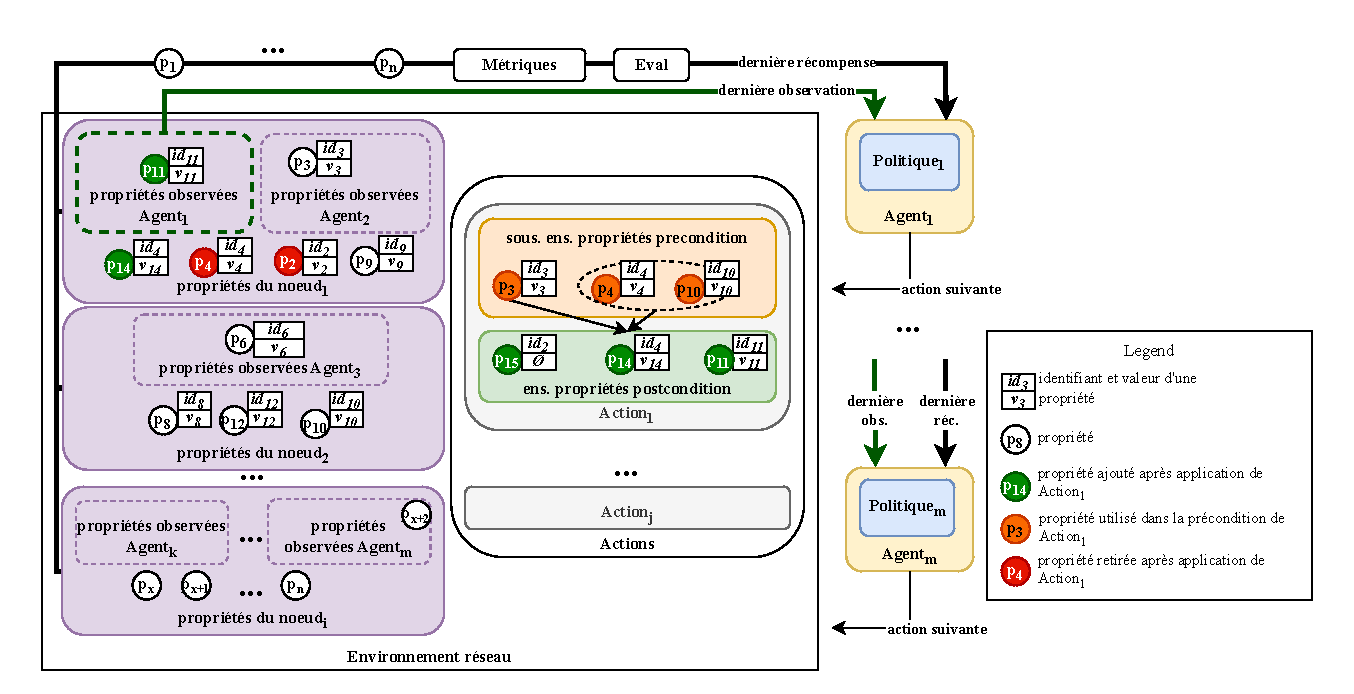
\includegraphics[trim=0.7cm 0.6cm 0.7cm 1cm, clip,width=1\textwidth]{figures/model_example_illustration.pdf}
    \caption{Vue illustrative du modèle de simulation}
    \label{fig:model_example_illustration}
\end{figure*}

\noindent
Le modèle \acn{Dec-POMDP} exprime l’état comme l’ensemble des propriétés des nœuds. Les actions sont définies par des pré/post-conditions sur ces propriétés. Les transitions et observations sont conditionnées par ces propriétés, et les récompenses sont calculées à partir de métriques sur l’état.

\subsubsection{Modélisation formelle Dec-POMDP}

Nous définissons les éléments liés aux propriétés des nœuds, des agents et des actions de l'environnement suivant :

\begin{itemize}

    \item $Ag = \{ag_1,..,ag_{|Ag|}\}$ : ensemble des agents (cyberattaquants et cyberdéfenseurs).
          % \begin{itemize}
          %     \item Avec $Attackers \subseteq Ag$ : l'ensemble des agents attaquants
          %     \item Avec $Defenders \subseteq Ag$ : l'ensemble des agents défenseurs
          % \end{itemize}

    \item Nous appelons le couple $p = (id_{j}, v_{j})$ avec $id_j \in {ID}$ et $v_j \in V$, une propriété.
          \begin{itemize}
              \item $\acn{ID}$ : l'ensemble des identifiants de propriétés indiquant éventuellement comment les propriétés sont organisées dans une structure de données non plate (telle que $PC1.processes.agents.agent1$). Ces identifiants de propriétés peuvent être utilisés pour un chemin d'accès à un fichier, le type de système d'exploitation utilisé dans un nœud, une ligne de commande utilisée par un agent\dots
              \item $V$ : Ensemble des valeurs de propriétés. Celles-ci peuvent inclure le contenu d'un fichier, une description complète du système d'exploitation, le résultat d'une ligne de commande\dots
                    % \item $Valeurs : \acn{ID} \rightarrow \mathcal{P}(V) = \{(id_{j}, V_{j}) \: | \: id_j \in {ID},$ $V_j \in \mathcal{P}(V)\}$ : une bijection associant un identifiant de propriété à l'ensemble des différentes valeurs auxquelles il peut être associé. Par exemple, l'identifiant $ls\_command\_output$ peut être associé aux valeurs suivantes $\{file.txt,\{file.txt,passwd.txt\}\}$
          \end{itemize}

    \item $P_{j} = \{ p_1, .., p_{|P_{j}|} \}$ : l'ensemble des propriétés $p_{l}$ (avec $l \in \{1,..,|P_{j}|\}$) du nœud $j$ ($j \in \mathbb{N} $). Par exemple, ces propriétés peuvent inclure certains identifiants de processus en cours d'exécution, la liste des fichiers d'un dossier, le type de système d'exploitation avec une description, des connaissances spécifiques d'un agent, etc.
          \begin{itemize}
              \item $P = P_1 \cup P_2 .. \cup P_{|P|} $ : Ensemble de toutes les propriétés des nœuds.
          \end{itemize}

    \item $Obs : \mathcal{P}(P) \times Ag \rightarrow \mathcal{P}(P_{Ag}), P_{Ag} \subset P$ : Relation qui associe les propriétés des nœuds et un agent au sous-ensemble de propriétés observées par l'agent.



    \item $Action : P_{pre} \rightarrow P_{post}$ : Relation qui associe un sous-ensemble de propriétés implicite dans une pré-condition booléenne conjonctive équivalente ($P_{pre} \subset \mathcal{P}(P)$) à un sous-ensemble de toutes les propriétés de la post-condition ($P_{post} \in \mathcal{P}(P)$). Par exemple, les propriétés $p_1 = (agent\_X\_privilege\_level, \allowbreak root)$, $p_2 = (agent\_X\_accessed\_text\_editor, \allowbreak Vim)$ et $p_3 = (agent\_X\_bashrc\_known\_filepath, \allowbreak /home/user/.bashrc)$ peuvent former une pré-condition ($p_1 \land p_2 \land p_3$) pour associer un nouvel ensemble de propriétés contenant $p4 = (bashrc\_file\_modified\_by\_X\_agent, \top)$. Deux sous-ensembles de pré-conditions peuvent être associés au même sous-ensemble de post-conditions pour modéliser une disjonction booléenne.

    \item $Metrics: \mathcal{P}(P) \times A \rightarrow \mathbb{R}^{n}$ : donne des métriques associées à un ensemble de propriétés et à une action conjointe. Par exemple, le nombre de nœuds encore actifs, les mouvements latéraux, etc.

\end{itemize}


En utilisant la description formelle d'un \acn{Dec-POMDP}~\cite{Oliehoek2016}, nous proposons le modèle \acn{Dec-POMDP} pré-spécialisé suivant :

\begin{itemize}
    \item $S = \{s_1, ..s_{|S|}\}, s_{i} \subseteq P \: et \: 1 \le i \le |S|$ : L'espace des états en tant qu'ensembles de propriétés possibles.

    \item $A_{i} = \{a_{i}^{1},..,a_{i}^{|A_{i}|}\}, a_{i}^j \in Action \: et \: 1 \le j \le |A_i|$ : l'ensemble des actions possibles pour l'agent $i$.

    \item $T$ : Ensemble des probabilités de transition conditionnelles entre les états
          \begin{itemize}
              \item Avec $T(s,a,s') = \probP(s'|s,a)$, la relation qui associe la probabilité d'aller de l'état $s \in S$ à l'état $s' \in S$ sachant que nous avons joué $a = (P^a_{pre} \times P^a_{post}) \in A$ avec $P^a_{pre} \subset \mathcal{P}(P)$ et $P^a_{post} \in \mathcal{P}(P)$
              \item Avec $\probP(s'|s,a) = 0$ si $s$ ne satisfait pas la condition préalable de $a$ (c'est-à-dire $\exists \: P_{pre_s}^{a} \in P_{pre}^{a} \: | \: P_{pre_s}^{a} \not\in \mathcal{P}(s)$).
              \item Avec $s' = (s - \{p_l=(id_l, v_l) \: | \: p_l \in s \: et$ $id_l \in \{id_k \: | \: (id_k, v_k) \in P^a_{post} \: et \: v_k \neq \varnothing\}\}) \cup P^a_{post}$
          \end{itemize}



    \item $R : S \times A \rightarrow \mathbb{R}^2 = Eval \circ Metrics$ : La fonction de récompense qui prend un état et une action et associe un indicateur de performance (à l'aide des métriques de l'état) pour les attaquants et les défenseurs.
          \begin{itemize}
              \item Avec $Eval : \mathbb{R}^{n} \rightarrow \mathbb{R}^2$, associe un vecteur métrique à une récompense pour les cyberattaquants et les cyberdéfenseurs.
          \end{itemize}



    \item $\Omega_{i} \subset Range(Obs \: | \: \{ (s, ag_i) | s \in S \: et \: ag_i \in Ag \}) \subset P$ : ensemble des propriétés observables pour l'agent $ag_i$. Par exemple, le contenu d'un fichier, la sortie du journal d'une commande, le résultat d'un scan de port, etc.
          \begin{itemize}
              \item $\Omega = \Omega_1 \cup \Omega_2 .. \cup \Omega_{|Ag|} = Range(Obs)$ : Ensemble de toutes les propriétés observables pour tous les agents.
          \end{itemize}

    \item $O$ : Ensemble des probabilités d'observation conditionnelles.
          \begin{itemize}
              \item Avec $O(s',a,o) = \probP(o|s',a)$, la relation qui associe la probabilité d'observer une observation $o \subset \Omega$ à partir de l'état $s' \in S$ induit par $a \in A$
              \item Avec $\probP(o|s',a) = 0$ si l'état $s' \in S$ ne contient pas les propriétés de $o \subset \Omega$ (c'est-à-dire $o \not\in \mathcal{P}(s')$). Par exemple, un agent joue l'action $x\_reads\_a\_log\_file$, ce qui donne lieu à un nouvel état dont une propriété appartenant à la connaissance de l'agent x est $(log\_file\_content\_known\_by\_x, \allowbreak abc)$. Cette propriété sera donc incluse dans les observations renvoyées à l'agent x.
          \end{itemize}

\end{itemize}


\subsubsection{Intégration des scénarios d’attaque/défense}

Pour intégrer des scénarios réalistes, on s’appuie sur MITRE ATT\&CK qui constitue une base de connaissances exhaustive des tactiques, techniques et procédures (\acn{TTP}) utilisées par les cyberattaquants.
Chaque \acn{TTP} est modélisée comme une action dans le \acn{Dec-POMDP}, avec des préconditions basées sur les propriétés requises et des post-conditions reflétant les effets de l’action.
Les mesures de détection et d’atténuation sont également intégrées comme des actions, permettant de simuler les réponses des défenseurs:
\begin{enumerate*}[label=\arabic*),itemjoin={;\quad}]
    \item Identifier tactiques/techniques/procédures pertinentes pour l’\acn{APT} ciblée.
    \item Décrire le scénario d’attaque/défense et la topologie réseau.
    \item Construire une arborescence \acn{AD}, chaque action étant définie par ses pré/post-conditions.
    \item Ajouter les mesures de détection/atténuation issues de MITRE ATT\&CK, également modélisées par des actions.
\end{enumerate*}

Ce formalisme permet de générer un simulateur multi-agents fidèle, où chaque action et observation est explicitement définie, facilitant l’extension à divers contextes de cyberdéfense.


\section{Description et mise en oeuvre dans l'activité}
% Présenter l’algorithme générique de l’activité de modélisation (inputs → outputs).
% Inclure le pseudo-code / algorithme en environnement LaTeX comme dans l’ancien chapitre.

L’algorithme \ref{alg:modeling} décrit le déroulement général de l’activité de modélisation.
Chaque étape est explicitée ci-dessous afin d’en préciser les objectifs et le rôle dans la construction du modèle final.

\paragraph{Étape 1 : Formalisation manuelle des fonctions composantes.}
La première étape consiste à dériver manuellement, à partir des descriptions informelles de l’objectif global et des contraintes organisationnelles, trois fonctions fondamentales : la fonction de récompense $R^j_H$, la fonction d’arrêt $S^j_H$, et la fonction de rendu optionnelle $Render^j_H$.
Cette étape requiert l’expertise des concepteurs, qui doivent transformer des objectifs de haut niveau (souvent exprimés en langage naturel ou sous forme de règles métiers) en spécifications formelles permettant l’évaluation de trajectoires dans l’environnement simulé.

\paragraph{Étape 2 : Entraînement des auto-encodeurs pour les observations.}
Une fois les historiques d’interactions collectés, les observations conjointes $\Omega^j$ en sont extraites.
Comme leur dimension peut être très élevée dans un contexte multi-agent, elles sont compressées à l’aide d’auto-encodeurs.
L’encodeur $Enc_{\omega^j}$ apprend à transformer les observations en représentations latentes compactes $z_t$, tandis que le décodeur $Dec_{\omega^j}$ reconstruit les observations originales à partir de ces latents.
L’objectif est de minimiser l’erreur de reconstruction, garantissant ainsi que les latents conservent l’information essentielle.

\paragraph{Étape 3 : Encodage des observations dans les historiques.}
Les auto-encodeurs entraînés sont ensuite utilisés pour transformer l’ensemble des historiques $\mathcal{D}_{H^j}$ en séquences d’états latents.
Chaque observation $\omega_t^j$ est convertie en une représentation $z_t$, ce qui permet de constituer un nouvel ensemble d’entraînement $\mathcal{B}$ composé de triplets $(z_t, a_t^j, z_{t+1})$.
Cet encodage réduit la complexité des données d’entrée et prépare l’entraînement du modèle de dynamique.

\paragraph{Étape 4 : Entraînement du modèle de dynamique récurrent (RLDM).}
À partir de l’ensemble encodé $\mathcal{B}$, un modèle récurrent de dynamique latente (\acn{RLDM}) est entraîné.
Ce modèle, noté $\mathcal{T}^z$, apprend à prédire l’évolution des états latents en fonction de l’historique caché $\tilde{h}_{t-1}$, de l’état encodé courant $z_t$, et de l’action conjointe $a_t^j$.
L’entraînement se fait en minimisant l’erreur quadratique moyenne entre la prédiction $\hat{z}_{t+1}$ et le latent réel $z_{t+1}$.
Ce mécanisme d’apprentissage permet de capturer la dynamique de l’environnement sans accès direct à l’état global.

\paragraph{Étape 5 : Construction du JOPM.}
Une fois le \acn{RLDM} entraîné, les observations initiales $\Omega^{\mathcal{T}^j}_0$ sont extraites des historiques et utilisées pour initialiser le simulateur.
Le modèle de transition conjoint $\mathcal{T}^j$ est alors défini en combinant le modèle récurrent $f$, l’encodeur $Enc$, et le décodeur $Dec$.
Ainsi, pour toute observation et action donnée, $\mathcal{T}^j$ met à jour l’état caché et génère une observation prédite, constituant ainsi un simulateur complet des interactions multi-agents.

\paragraph{Étape 6 : Sorties de l’activité.}
Enfin, l’activité retourne l’ensemble des éléments modélisés : le modèle de transition conjoint $\mathcal{T}^j$, l’ensemble des observations initiales $\Omega^{\mathcal{T}^j}_0$, la fonction de récompense $R^j_H$, la fonction d’arrêt $S^j_H$, et la fonction de rendu éventuelle $Render^j_H$.
Ces composants constituent le cœur du jumeau numérique qui sera exploité par les activités d’entraînement, d’analyse et de transfert de la méthode \acn{MAMAD}.


\begin{algorithm}[H]
    \caption{Algorithme de l'activité de modélisation}
    \label{alg:modeling}
    \DontPrintSemicolon

    \KwIn{Historiques conjoints $\mathcal{D}_{H^j}$, objectif informel $\mathcal{G}_{\text{inf}}$, contraintes informelles $\mathcal{C}_{\text{inf}}$, facteur d'actualisation $\gamma$, espace des actions $A$, espace des observations $\Omega$}
    \KwOut{\acn{JOPM} $\mathcal{T}^j$, fonction de récompense $R^j_H$, spécifications MOISE+MARL $\mathcal{MM}$}

    \vspace{0.5em}
    \tcp{1. Formalisation manuelle des fonctions composantes}
    $(R^j_H, S^j_H, \text{Render}^j_H) \gets \texttt{manual\_formalize}(\mathcal{S}_{\text{inf}}, \mathcal{G}_{\text{inf}}, \mathcal{E}, A, \Omega)$ \;

    \vspace{0.5em}
    \tcp{2. Entraîner les auto-encodeurs pour les observations}
    Extraire les observations $\Omega^j = \{\omega^j_t\}$ à partir des historiques $\mathcal{D}_{H^j}$ \;
    Entraîner un auto-encodeur $(Enc_{\omega^j}, Dec_{\omega^j})$ sur $\Omega^j$ en minimisant l'erreur de reconstruction \;

    \vspace{0.5em}
    \tcp{3. Encoder les observations dans les historiques}
    Pour chaque historique $h^j = (\omega_t^j, a_t^j) \in \mathcal{D}_{H^j}$, encoder chaque observation conjointe ${z}_t = Enc_{\omega^j}(\omega^j_t)$ pour constituer l'ensemble d'entraînement $\mathcal{B} = \{ \{(z_t, a^j_t, z_{t+1})\} = h_z^j, h_z^j \in \mathcal{D}_{H^j}\}$

    \vspace{0.5em}
    \tcp{4. Entraîner le \acn{RLDM}}
    Initialiser le \acn{RLDM} $\mathcal{T}^z = f(g)$

    \For{$h_z^j \in \mathcal{B}$}{
        \For{$(z_t, a^j_t, z_{t+1}) \in h^j$}{
            Entraîner le \acn{RLDM} $\mathcal{T}^{z}$ en minimisant l'erreur quadratique moyenne (\acparen{MSE}) entre la prédiction $\hat{z}_{t+1}$ et la valeur réelle $z_{t+1}$.
        }
    }

    \vspace{0.5em}
    \tcp{5. Sauvegarder les observations initiales et former le JOPM}

    $\Omega^{\mathcal{T}^j}_0 \gets \{\omega^j_0\}$ extraites des historiques $\mathcal{D}_{H^j}$

    $\mathcal{T}^j(h_{t-1}, \omega_t, a_t) = \langle f(h_{t-1}, Enc(\omega^j_t), a^j_t), Dec(\mathcal{T}^{z}(h_{t-1}, Enc(\omega^j_t), a^j_t)) \rangle$ \;

    \vspace{0.5em}
    \tcp{6. Retourner les éléments modélisés}
    \Return{$\mathcal{T}^j, \Omega^{\mathcal{T}^j}_0, R^j_H, S^j_H, \text{Render}^j_H$}
\end{algorithm}



\section{Synthèse, limites et transition}

\noindent
En synthèse, l’activité de modélisation vise à fournir un environnement simulé fidèle et exploitable pour l’entraînement multi-agent, en combinant formalisme explicite (\acn{Dec-POMDP} générique) et génération automatique par World Models multi-agents. Les sorties produites — le modèle de transition conjoint (\acn{JOPM}), la fonction de récompense, la fonction d’arrêt et la fonction de rendu — constituent le socle du jumeau numérique utilisé dans les étapes suivantes. Cette approche permet d’assurer l’adaptation (via l’apprentissage sur données réelles), l’explicabilité (par la structure formelle du modèle) et la réutilisabilité (grâce au châssis générique). Toutefois, la fidélité du modèle dépend de la qualité et de la diversité des historiques collectés, et le coût computationnel de l’entraînement des auto-encodeurs et du \acn{RLDM} peut être élevé pour des environnements complexes. Enfin, la granularité des actions et la couverture des dynamiques réelles restent des limites inhérentes à toute simulation. L’activité d’entraînement exploitera ce modèle simulé pour optimiser les politiques sous contraintes organisationnelles, amorçant ainsi le cycle itératif de la méthode \acn{MAMAD}.

\clearpage
\thispagestyle{empty}
\null
\newpage

\chapter{Entraîner des politiques sous contraintes}
\label{chap:training}

L'\textit{activité d'entraînement} consiste à optimiser les politiques conjointes des agents dans l’environnement simulé, en tenant compte des contraintes organisationnelles.
Elle correspond à la phase de résolution du problème de conception, en exploitant les modèles produits par l’activité de modélisation.

Cette activité est cruciale car elle relie la performance (C2) et l’adaptation (C3) à l’explicabilité (C5) et au contrôle (C4), via l’intégration de contraintes explicites dans l’apprentissage multi-agent.

\section*{Objectifs formels}

Les \textbf{entrées} de l’activité d’entraînement sont :
\begin{itemize}
    \item le modèle de transition conjoint $\mathcal{T}^j$ produit par la modélisation ;
    \item les observations initiales $\Omega^{\mathcal{T}^j}_0$ ;
    \item la fonction de récompense $R^j_H$ et la fonction d’arrêt $S^j_H$ ;
    \item les spécifications organisationnelles $\mathcal{MM}$ issues des contraintes informelles $\mathcal{C}_{\text{inf}}$ ;
    \item les espaces d’observations $\Omega$ et d’actions $A$ ;
    \item le facteur d’actualisation $\gamma$.
\end{itemize}

La \textbf{sortie attendue} est :
\begin{itemize}
    \item une politique conjointe entraînée $\pi^j = \{\pi^j_0, \pi^j_1, \dots, \pi^j_n\}$.
\end{itemize}

\noindent La relation globale peut s’exprimer par :
\begin{displaymath}
    \pi^j \gets \texttt{train}(\mathcal{T}^j, \Omega^{\mathcal{T}^j}_0, R^j_H, S^j_H, \text{Render}^j_H, \mathcal{MM}, \mathcal{C}_{\text{inf}}, \gamma, \Omega, A)
\end{displaymath}
\section{Travaux mobilisés et verrous identifiés}

L’activité d’entraînement des politiques sous contraintes s’appuie sur plusieurs familles de travaux issus du domaine du \acn{MARL} et de l’intégration de contraintes organisationnelles.

Du côté du \acn{MARL}, les méthodes classiques telles que l’apprentissage indépendant, l’apprentissage centralisé avec exécution décentralisée (\acn{CTDE}), ou encore les algorithmes de type Q-learning, Policy Gradient et leurs variantes multi-agents, constituent la base pour optimiser des politiques conjointes dans des environnements simulés. Ces approches sont efficaces pour maximiser la performance collective, mais elles n’intègrent pas nativement de contraintes organisationnelles explicites.

Pour pallier ce manque, plusieurs travaux issus du Safe \acn{RL} et des Constrained MDPs (\acn{CMDP}) ont été mobilisés. Les méthodes comme Constrained Policy Optimization (\acn{CPO}) ou Deep Constrained Q-Learning (\acn{DCQL}) permettent d’intégrer des contraintes numériques (sûreté, consommation, risque) dans le processus d’apprentissage, mais leur expressivité reste limitée à des contraintes locales et numériques, sans prise en compte de structures organisationnelles complexes.

Les approches de reward shaping, shielding, ou feedback humain offrent des mécanismes de guidage souple, permettant d’influencer indirectement les politiques apprises. Cependant, elles ne garantissent pas le respect formel de contraintes organisationnelles et restent difficiles à interpréter.

Enfin, les travaux sur l’intégration de modèles organisationnels symboliques, tels que $\mathcal{M}OISE^+$, proposent une formalisation riche des rôles, missions et relations collectives. Toutefois, leur intégration directe dans le processus d’apprentissage \acn{MARL} reste un verrou majeur, en raison de la difficulté à traduire ces spécifications en contraintes opérationnelles exploitables par les algorithmes d’apprentissage.

En synthèse, les principaux verrous identifiés sont :
\begin{itemize}
    \item l’absence de cadre unifié permettant d’intégrer des contraintes organisationnelles symboliques dans l’apprentissage \acn{MARL} ;
    \item la difficulté à garantir le respect de ces contraintes tout en maintenant la performance et l’adaptabilité des politiques ;
    \item le manque d’explicabilité et de contrôle sur les politiques apprises dans des environnements complexes et dynamiques.
\end{itemize}

\section{Positionnement et contributions proposées}

Pour lever ces verrous, notre approche propose d’hybrider les forces des cadres symboliques et connexionnistes en introduisant le framework MOISE+MARL. Ce cadre permet d’intégrer explicitement des spécifications organisationnelles (rôles, missions, permissions, obligations) dans le processus d’apprentissage multi-agent, en les traduisant sous forme de guides de contraintes (action masking, shaping de récompense, guides d’objectifs) injectés dans les algorithmes \acn{MARL}.

Notre contribution principale consiste à :
\begin{itemize}
    \item formaliser l’intégration des spécifications organisationnelles $\mathcal{M}OISE^+$ dans le \acn{MARL} via des guides de contraintes, permettant de restreindre ou d’orienter l’espace des politiques apprises ;
    \item proposer un nouveau formalisme, l’\acn{ODec-POMDP}, compatible avec les environnements simulés appris (World Models), pour permettre l’entraînement à partir de données observables uniquement ;
    \item développer un algorithme d’entraînement générique (voir Algorithme~\ref{alg:training_mamad}) qui articule ces guides de contraintes avec les méthodes \acn{MARL} existantes, assurant ainsi la compatibilité entre apprentissage connexionniste et respect des contraintes organisationnelles ;
    \item offrir un certain degré d’explicabilité et de contrôle sur les politiques apprises, grâce à la traçabilité des guides de contraintes et à l’analyse post-hoc des comportements émergents.
\end{itemize}

Ce positionnement permet de concilier performance, adaptation, contrôle et explicabilité dans l’entraînement des politiques multi-agents sous contraintes, ouvrant la voie à une conception plus robuste et transparente des \acn{SMA} pour des environnements critiques comme la cyberdéfense.

\subsection{MOISE+MARL pour lier $\mathcal{M}OISE^+$ avec le MARL}

\begin{figure}[h!]
    \centering
    \tikzset{every picture/.style={line width=0.75pt}} %set default line width to 0.75pt        

\begin{tikzpicture}[x=0.75pt,y=0.75pt,yscale=-1.2,xscale=1.4]
    %uncomment if require: \path (0,2584); %set diagram left start at 0, and has height of 2584

    %Straight Lines [id:da4973066741986565] 
    \draw [line width=1.5]    (118.21,2302.58) -- (203.1,2302) ;
    %Straight Lines [id:da14807114776731778] 
    \draw    (368.35,2272) -- (368.35,2294) -- (332.16,2294) ;
    \draw [shift={(330.16,2294)}, rotate = 360] [color={rgb, 255:red, 0; green, 0; blue, 0 }  ][line width=0.75]    (6.56,-1.97) .. controls (4.17,-0.84) and (1.99,-0.18) .. (0,0) .. controls (1.99,0.18) and (4.17,0.84) .. (6.56,1.97)   ;
    %Straight Lines [id:da16285043353898754] 
    \draw [line width=1.5]    (83.88,2398) -- (204.61,2398) ;
    %Straight Lines [id:da6299512000169913] 
    \draw    (169.94,2348) -- (204.61,2348) ;
    %Straight Lines [id:da64750232417664] 
    \draw    (84.65,2446) -- (383.15,2446) ;
    %Straight Lines [id:da35895220906699743] 
    \draw    (84.65,2230) -- (383,2230) ;
    %Straight Lines [id:da715014372569708] 
    \draw    (244.68,2262) -- (224.68,2262) -- (224.68,2408) ;
    \draw [shift={(224.68,2410)}, rotate = 270] [color={rgb, 255:red, 0; green, 0; blue, 0 }  ][line width=0.75]    (6.56,-1.97) .. controls (4.17,-0.84) and (1.99,-0.18) .. (0,0) .. controls (1.99,0.18) and (4.17,0.84) .. (6.56,1.97)   ;
    %Straight Lines [id:da71870438525014] 
    \draw    (251.96,2328) -- (286.51,2328) -- (286.51,2356) ;
    \draw [shift={(286.51,2358)}, rotate = 270] [color={rgb, 255:red, 0; green, 0; blue, 0 }  ][line width=0.75]    (6.56,-1.97) .. controls (4.17,-0.84) and (1.99,-0.18) .. (0,0) .. controls (1.99,0.18) and (4.17,0.84) .. (6.56,1.97)   ;
    %Straight Lines [id:da6006267784187092] 
    \draw [line width=0.75]  [dash pattern={on 0.84pt off 2.51pt}]  (252.87,2378) -- (252.87,2407) ;
    \draw [shift={(252.87,2410)}, rotate = 270] [fill={rgb, 255:red, 0; green, 0; blue, 0 }  ][line width=0.08]  [draw opacity=0] (5.36,-2.57) -- (0,0) -- (5.36,2.57) -- cycle    ;
    %Straight Lines [id:da8743336135156266] 
    \draw    (322.88,2304) -- (322.88,2316) ;
    \draw [shift={(322.88,2318)}, rotate = 270] [color={rgb, 255:red, 0; green, 0; blue, 0 }  ][line width=0.75]    (6.56,-1.97) .. controls (4.17,-0.84) and (1.99,-0.18) .. (0,0) .. controls (1.99,0.18) and (4.17,0.84) .. (6.56,1.97)   ;
    %Straight Lines [id:da14641229967966152] 
    \draw [line width=0.75]  [dash pattern={on 0.84pt off 2.51pt}]  (322.88,2378) -- (322.88,2407) ;
    \draw [shift={(322.88,2410)}, rotate = 270] [fill={rgb, 255:red, 0; green, 0; blue, 0 }  ][line width=0.08]  [draw opacity=0] (5.36,-2.57) -- (0,0) -- (5.36,2.57) -- cycle    ;
    %Straight Lines [id:da9260929933425808] 
    \draw [line width=0.75]  [dash pattern={on 0.84pt off 2.51pt}]  (286.51,2378) -- (286.51,2420) -- (312.61,2420) ;
    \draw [shift={(315.61,2420)}, rotate = 180] [fill={rgb, 255:red, 0; green, 0; blue, 0 }  ][line width=0.08]  [draw opacity=0] (5.36,-2.57) -- (0,0) -- (5.36,2.57) -- cycle    ;
    %Straight Lines [id:da3057006030233673] 
    \draw [line width=0.75]  [dash pattern={on 0.84pt off 2.51pt}]  (274,2449.7) -- (274,2457) ;
    \draw [shift={(274,2460)}, rotate = 270] [fill={rgb, 255:red, 0; green, 0; blue, 0 }  ][line width=0.08]  [draw opacity=0] (3.57,-1.72) -- (0,0) -- (3.57,1.72) -- cycle    ;
    %Straight Lines [id:da07288166228322246] 
    \draw    (342,2449.98) -- (342,2458) ;
    \draw [shift={(342,2460)}, rotate = 270] [color={rgb, 255:red, 0; green, 0; blue, 0 }  ][line width=0.75]    (6.56,-1.97) .. controls (4.17,-0.84) and (1.99,-0.18) .. (0,0) .. controls (1.99,0.18) and (4.17,0.84) .. (6.56,1.97)   ;
    %Shape: Ellipse [id:dp8508274348425935] 
    \draw   (95.09,2288.86) .. controls (95.09,2287.28) and (96.33,2286) .. (97.85,2286) .. controls (99.38,2286) and (100.62,2287.28) .. (100.62,2288.86) .. controls (100.62,2290.44) and (99.38,2291.71) .. (97.85,2291.71) .. controls (96.33,2291.71) and (95.09,2290.44) .. (95.09,2288.86) -- cycle ;
    %Straight Lines [id:da3825450168053828] 
    \draw    (97.85,2291.71) -- (97.85,2298.86) ;
    %Straight Lines [id:da521321206042058] 
    \draw    (97.85,2298.86) -- (93.71,2306) ;
    %Straight Lines [id:da055514206493922025] 
    \draw    (97.85,2298.86) -- (102,2306) ;
    %Straight Lines [id:da8996496708356774] 
    \draw    (102,2294.57) -- (93.71,2294.57) ;

    %Straight Lines [id:da31678488015771755] 
    \draw [line width=2.25]    (188,2454) -- (196.97,2454) ;
    \draw [shift={(201.97,2454)}, rotate = 180] [fill={rgb, 255:red, 0; green, 0; blue, 0 }  ][line width=0.08]  [draw opacity=0] (5.72,-2.75) -- (0,0) -- (5.72,2.75) -- cycle    ;
    %Shape: Ellipse [id:dp3927356466672782] 
    \draw   (238.88,2451.17) .. controls (238.88,2450.36) and (239.67,2449.7) .. (240.64,2449.7) .. controls (241.61,2449.7) and (242.4,2450.36) .. (242.4,2451.17) .. controls (242.4,2451.99) and (241.61,2452.65) .. (240.64,2452.65) .. controls (239.67,2452.65) and (238.88,2451.99) .. (238.88,2451.17) -- cycle ;
    %Straight Lines [id:da3365602555559104] 
    \draw    (240.64,2452.65) -- (240.64,2456.32) ;
    %Straight Lines [id:da7990875235744026] 
    \draw    (240.64,2456.32) -- (238,2460) ;
    %Straight Lines [id:da23945649338821617] 
    \draw    (240.64,2456.32) -- (243.28,2460) ;
    %Straight Lines [id:da11927353559661591] 
    \draw    (243.28,2454.12) -- (238,2454.12) ;

    %Straight Lines [id:da5816423191130675] 
    \draw    (251.96,2272) -- (252.85,2356) ;
    \draw [shift={(252.87,2358)}, rotate = 269.39] [color={rgb, 255:red, 0; green, 0; blue, 0 }  ][line width=0.75]    (6.56,-1.97) .. controls (4.17,-0.84) and (1.99,-0.18) .. (0,0) .. controls (1.99,0.18) and (4.17,0.84) .. (6.56,1.97)   ;
    %Straight Lines [id:da9310455126832857] 
    \draw    (321.97,2338) -- (321.97,2356) ;
    \draw [shift={(321.97,2358)}, rotate = 270] [color={rgb, 255:red, 0; green, 0; blue, 0 }  ][line width=0.75]    (6.56,-1.97) .. controls (4.17,-0.84) and (1.99,-0.18) .. (0,0) .. controls (1.99,0.18) and (4.17,0.84) .. (6.56,1.97)   ;
    %Shape: Rectangle [id:dp293492578719597] 
    \draw   (120,2453) .. controls (120,2451.34) and (121.34,2450) .. (123,2450) -- (127.72,2450) .. controls (129.37,2450) and (130.72,2451.34) .. (130.72,2453) -- (130.72,2457) .. controls (130.72,2458.66) and (129.37,2460) .. (127.72,2460) -- (123,2460) .. controls (121.34,2460) and (120,2458.66) .. (120,2457) -- cycle ;
    %Straight Lines [id:da33566712615128225] 
    \draw    (261.05,2262) -- (306,2262) ;
    \draw [shift={(308,2262)}, rotate = 180] [color={rgb, 255:red, 0; green, 0; blue, 0 }  ][line width=0.75]    (6.56,-1.97) .. controls (4.17,-0.84) and (1.99,-0.18) .. (0,0) .. controls (1.99,0.18) and (4.17,0.84) .. (6.56,1.97)   ;
    %Shape: Rectangle [id:dp28383270948937667] 
    \draw   (308,2236) -- (381.08,2236) -- (381.08,2276) -- (308,2276) -- cycle ;
    %Straight Lines [id:da18020989903965012] 
    \draw [line width=3]    (97.22,2282) -- (97.22,2270) ;
    \draw [shift={(97.22,2264)}, rotate = 90] [fill={rgb, 255:red, 0; green, 0; blue, 0 }  ][line width=0.08]  [draw opacity=0] (10.18,-4.89) -- (0,0) -- (10.18,4.89) -- cycle    ;
    %Straight Lines [id:da018421338049046554] 
    \draw [line width=3]    (97.22,2310) -- (97.11,2322.37) ;
    \draw [shift={(97.22,2328)}, rotate = 268.86] [fill={rgb, 255:red, 0; green, 0; blue, 0 }  ][line width=0.08]  [draw opacity=0] (10.18,-4.89) -- (0,0) -- (10.18,4.89) -- cycle    ;
    %Shape: Rectangle [id:dp7281037051878541] 
    \draw   (85.42,2450) -- (96.13,2450) -- (96.13,2460) -- (85.42,2460) -- cycle ;

    % Text Node
    \draw (362,2544.5) node  [font=\tiny] [align=left] {Role to constraint guide};
    % Text Node
    \draw (342,2524.5) node  [font=\tiny] [align=left] {Agents set};
    % Text Node
    \draw (342,2504.5) node  [font=\tiny] [align=left] {Actions set};
    % Text Node
    \draw (257,2584.5) node  [font=\tiny] [align=left] {Goal to constraint guide};
    % Text Node
    \draw (335,2484.5) node  [font=\tiny] [align=left] {Goals};
    % Text Node
    \draw (359,2564.5) node  [font=\tiny] [align=left] {Role to deontic specs.};
    % Text Node
    \draw (232,2564.5) node  [font=\tiny] [align=left] {Mission};
    % Text Node
    \draw (245,2544.5) node  [font=\tiny] [align=left] {Reward function};
    % Text Node
    \draw (248,2524.5) node  [font=\tiny] [align=left] {Goal-reward guide};
    % Text Node
    \draw (242,2504.5) node  [font=\tiny] [align=left] {Mission weight};
    % Text Node
    \draw (245,2484.5) node  [font=\tiny] [align=left] {Time constraints};
    % Text Node
    \draw (127,2584.5) node  [font=\tiny] [align=left] {Mission to goals};
    % Text Node
    \draw (129,2564.5) node  [font=\tiny] [align=left] {Role-reward guide};
    % Text Node
    \draw (128,2544.5) node  [font=\tiny] [align=left] {Role-action guide};
    % Text Node
    \draw (121,2524.5) node  [font=\tiny] [align=left] {Agent to role};
    % Text Node
    \draw (115,2504.5) node  [font=\tiny] [align=left] {Roles set};
    % Text Node
    \draw (122,2484.5) node  [font=\tiny] [align=left] {Deontic specs.};
    % Text Node
    \draw (310,2544) node  [font=\tiny] [align=left] {$\displaystyle \boldsymbol{rcg}$};
    % Text Node
    \draw (200,2504) node  [font=\tiny] [align=left] {$\displaystyle \mathcal{P}$};
    % Text Node
    \draw (200,2484) node  [font=\tiny] [align=left] {$\displaystyle \mathcal{T_{C}}$};
    % Text Node
    \draw (200,2564) node  [font=\tiny] [align=left] {$\displaystyle \mathcal{M}$};
    % Text Node
    \draw (77.5,2484) node  [font=\tiny] [align=left] {$\displaystyle \mathcal{DS}$};
    % Text Node
    \draw (310,2564) node  [font=\tiny] [align=left] {$\displaystyle \boldsymbol{rds}$};
    % Text Node
    \draw (310,2504) node  [font=\tiny] [align=left] {$\displaystyle \boldsymbol{A}$};
    % Text Node
    \draw (200,2544) node  [font=\tiny] [align=left] {$\displaystyle \boldsymbol{R}$};
    % Text Node
    \draw (310,2524) node  [font=\tiny] [align=left] {$\displaystyle \mathcal{A}$};
    % Text Node
    \draw (200,2524) node  [font=\tiny] [align=left] {$\displaystyle \boldsymbol{grg}$};
    % Text Node
    \draw (77.5,2564) node  [font=\tiny] [align=left] {$\displaystyle \boldsymbol{rrg}$};
    % Text Node
    \draw (77.5,2544) node  [font=\tiny] [align=left] {$\displaystyle \boldsymbol{rag}$};
    % Text Node
    \draw (200,2584) node  [font=\tiny] [align=left] {$\displaystyle \boldsymbol{gcg}$};
    % Text Node
    \draw (76.5,2524) node  [font=\tiny] [align=left] {$\displaystyle \boldsymbol{ar}$};
    % Text Node
    \draw (77,2584) node  [font=\tiny] [align=left] {$\displaystyle \boldsymbol{mo}$};
    % Text Node
    \draw (76.5,2504) node  [font=\tiny] [align=left] {$\displaystyle \mathcal{R}$};
    % Text Node
    \draw (310,2484) node  [font=\tiny] [align=left] {$\displaystyle \mathcal{G}$};


    % Text Node
    \draw  [fill={rgb, 255:red, 255; green, 255; blue, 255 }  ,fill opacity=1 ]  (241.82,2323) .. controls (241.82,2320.24) and (244.06,2318) .. (246.82,2318) -- (259.82,2318) .. controls (262.58,2318) and (264.82,2320.24) .. (264.82,2323) -- (264.82,2333) .. controls (264.82,2335.76) and (262.58,2338) .. (259.82,2338) -- (246.82,2338) .. controls (244.06,2338) and (241.82,2335.76) .. (241.82,2333) -- cycle  ;
    \draw (253.32,2328) node  [font=\scriptsize] [align=left] {$\displaystyle \boldsymbol{rcg}$};
    % Text Node
    \draw    (337,2252) -- (354,2252) -- (354,2272) -- (337,2272) -- cycle  ;
    \draw (345.5,2262) node  [font=\scriptsize] [align=left] {$\displaystyle \mathcal{Y}$};
    % Text Node
    \draw    (311,2252) -- (334,2252) -- (334,2272) -- (311,2272) -- cycle  ;
    \draw (322.5,2262) node  [font=\scriptsize] [align=left] {$\displaystyle \mathcal{T_{C}}$};
    % Text Node
    \draw    (357.39,2252) -- (378.39,2252) -- (378.39,2272) -- (357.39,2272) -- cycle  ;
    \draw (367.89,2262) node  [font=\scriptsize] [align=left] {$\displaystyle \mathcal{M}$};
    % Text Node
    \draw (347.43,2244) node  [font=\scriptsize] [align=left] {$\displaystyle \mathcal{DS}$};
    % Text Node
    \draw  [fill={rgb, 255:red, 255; green, 255; blue, 255 }  ,fill opacity=1 ]  (270,2257) .. controls (270,2254.24) and (272.24,2252) .. (275,2252) -- (288,2252) .. controls (290.76,2252) and (293,2254.24) .. (293,2257) -- (293,2267) .. controls (293,2269.76) and (290.76,2272) .. (288,2272) -- (275,2272) .. controls (272.24,2272) and (270,2269.76) .. (270,2267) -- cycle  ;
    \draw (281.5,2262) node  [font=\scriptsize] [align=left] {$\displaystyle \boldsymbol{rds}$};
    % Text Node
    \draw (158,2454.5) node  [font=\tiny] [align=left] {Relation name};
    % Text Node
    \draw (106.46,2454.5) node  [font=\tiny] [align=left] {Set};
    % Text Node
    \draw (255.47,2454.5) node  [font=\tiny] [align=left] {User};
    % Text Node
    \draw (216.32,2454.5) node  [font=\tiny] [align=left] {Define};
    % Text Node
    \draw (366.91,2454.5) node  [font=\tiny] [align=left] {Set relation};
    % Text Node
    \draw (306.61,2454.5) node  [font=\tiny] [align=left] {Impact on training};
    % Text Node
    \draw    (244.82,2410) -- (261.82,2410) -- (261.82,2430) -- (244.82,2430) -- cycle  ;
    \draw (253.32,2420) node  [font=\scriptsize] [align=left] {$\displaystyle \boldsymbol{A}$};
    % Text Node
    \draw    (314.84,2410) -- (331.84,2410) -- (331.84,2430) -- (314.84,2430) -- cycle  ;
    \draw (323.34,2420) node  [font=\scriptsize] [align=left] {$\displaystyle \boldsymbol{R}$};
    % Text Node
    \draw    (215.63,2410) -- (234.63,2410) -- (234.63,2430) -- (215.63,2430) -- cycle  ;
    \draw (225.13,2420) node  [font=\scriptsize] [align=left] {$\displaystyle \mathcal{A}$};
    % Text Node
    \draw  [fill={rgb, 255:red, 255; green, 255; blue, 255 }  ,fill opacity=1 ]  (309.97,2363) .. controls (309.97,2360.24) and (312.21,2358) .. (314.97,2358) -- (328.97,2358) .. controls (331.73,2358) and (333.97,2360.24) .. (333.97,2363) -- (333.97,2373) .. controls (333.97,2375.76) and (331.73,2378) .. (328.97,2378) -- (314.97,2378) .. controls (312.21,2378) and (309.97,2375.76) .. (309.97,2373) -- cycle  ;
    \draw (321.97,2368) node  [font=\scriptsize] [align=left] {$\displaystyle \boldsymbol{grg}$};
    % Text Node
    \draw    (274.56,2363) .. controls (274.56,2360.24) and (276.8,2358) .. (279.56,2358) -- (292.56,2358) .. controls (295.32,2358) and (297.56,2360.24) .. (297.56,2363) -- (297.56,2373) .. controls (297.56,2375.76) and (295.32,2378) .. (292.56,2378) -- (279.56,2378) .. controls (276.8,2378) and (274.56,2375.76) .. (274.56,2373) -- cycle  ;
    \draw (286.06,2368) node  [font=\scriptsize] [align=left] {$\displaystyle \boldsymbol{rrg}$};
    % Text Node
    \draw    (240.87,2363) .. controls (240.87,2360.24) and (243.11,2358) .. (245.87,2358) -- (259.87,2358) .. controls (262.63,2358) and (264.87,2360.24) .. (264.87,2363) -- (264.87,2373) .. controls (264.87,2375.76) and (262.63,2378) .. (259.87,2378) -- (245.87,2378) .. controls (243.11,2378) and (240.87,2375.76) .. (240.87,2373) -- cycle  ;
    \draw (252.87,2368) node  [font=\scriptsize] [align=left] {$\displaystyle \boldsymbol{rag}$};
    % Text Node
    \draw (156.15,2380.5) node  [font=\footnotesize] [align=left] {$\displaystyle  \begin{array}{{>{\displaystyle}l}}
                \ \ \boldsymbol{Constraint\ Guides} \\
                ( roles\ and\ goals\ logic)
            \end{array}$};
    % Text Node
    \draw  [fill={rgb, 255:red, 255; green, 255; blue, 255 }  ,fill opacity=1 ]  (309.93,2323) .. controls (309.93,2320.24) and (312.17,2318) .. (314.93,2318) -- (329.93,2318) .. controls (332.69,2318) and (334.93,2320.24) .. (334.93,2323) -- (334.93,2333) .. controls (334.93,2335.76) and (332.69,2338) .. (329.93,2338) -- (314.93,2338) .. controls (312.17,2338) and (309.93,2335.76) .. (309.93,2333) -- cycle  ;
    \draw (322.43,2328) node  [font=\scriptsize] [align=left] {$\displaystyle \boldsymbol{gcg}$};
    % Text Node
    \draw  [fill={rgb, 255:red, 255; green, 255; blue, 255 }  ,fill opacity=1 ]  (214.77,2323) .. controls (214.77,2320.24) and (217.01,2318) .. (219.77,2318) -- (227.77,2318) .. controls (230.53,2318) and (232.77,2320.24) .. (232.77,2323) -- (232.77,2333) .. controls (232.77,2335.76) and (230.53,2338) .. (227.77,2338) -- (219.77,2338) .. controls (217.01,2338) and (214.77,2335.76) .. (214.77,2333) -- cycle  ;
    \draw (223.77,2328) node  [font=\scriptsize] [align=left] {$\displaystyle \boldsymbol{ar}$};
    % Text Node
    \draw  [fill={rgb, 255:red, 255; green, 255; blue, 255 }  ,fill opacity=1 ]  (356.85,2289) .. controls (356.85,2286.24) and (359.08,2284) .. (361.85,2284) -- (374.85,2284) .. controls (377.61,2284) and (379.85,2286.24) .. (379.85,2289) -- (379.85,2299) .. controls (379.85,2301.76) and (377.61,2304) .. (374.85,2304) -- (361.85,2304) .. controls (359.08,2304) and (356.85,2301.76) .. (356.85,2299) -- cycle  ;
    \draw (368.35,2294) node  [font=\scriptsize] [align=left] {$\displaystyle \boldsymbol{mo}$};
    % Text Node
    \draw (127,2344.5) node  [font=\small] [align=left] {$\displaystyle  \begin{array}{{>{\displaystyle}l}}
                \mathbf{MOISE\ +MARL} \\
                \mathbf{Specs.\ Level}
            \end{array}$};
    % Text Node
    \draw (127,2422.5) node  [font=\small] [align=left] {$\displaystyle  \begin{array}{{>{\displaystyle}l}}
                \mathbf{MARL\ Level} \\
                \mathbf{(Dec-POMDP)}
            \end{array}$};
    % Text Node
    \draw    (243.91,2252) -- (260.91,2252) -- (260.91,2272) -- (243.91,2272) -- cycle  ;
    \draw (252.41,2262) node  [font=\scriptsize] [align=left] {$\displaystyle \mathcal{R}$};
    % Text Node
    \draw (182.64,2315) node  [font=\footnotesize] [align=left] {$\displaystyle \boldsymbol{Linkers}$};
    % Text Node
    \draw    (313.93,2284) -- (330.93,2284) -- (330.93,2304) -- (313.93,2304) -- cycle  ;
    \draw (322.43,2294) node  [font=\scriptsize] [align=left] {$\displaystyle \mathcal{G}$};
    % Text Node
    \draw (127,2261.5) node  [font=\small] [align=left] {$\displaystyle  \begin{array}{{>{\displaystyle}l}}
                \mathbf{{\displaystyle Org.\ Specs.\ Level}} \\
                {\displaystyle \ \ \ \ \ \ \ \ \ \ \ (\mathcal{M}\mathbf{OISE^+})}
            \end{array}$};


\end{tikzpicture}
    \caption[Vue minimale du framework MOISE+MARL]{Vue minimale du framework MOISE+MARL~: Les utilisateurs définissent d'abord les spécifications $\mathcal{M}OISE^+$, qui incluent les rôles ($\mathcal{R}$) et les missions ($\mathcal{M}$), tous deux associés via $rds$. Ils créent ensuite les spécifications MOISE+MARL en définissant d'abord des guides de contraintes tels que $rag$ et $rrg$ pour spécifier la logique des rôles, et $grg$ pour la logique des objectifs. Des linkers sont ensuite utilisés pour connecter les agents aux rôles via $ar$ et pour lier la logique des guides de contraintes aux spécifications $\mathcal{M}OISE^+$ définies. Une fois ces éléments configurés, les rôles peuvent être attribués aux agents, et le framework \acn{MARL} est mis à jour en conséquence pendant l'apprentissage.
    }
    \label{fig:mm_synthesis}
\end{figure}

\noindent MOISE+MARL introduit des moyens de contrôler ou de guider l'apprentissage des agents en \acn{MARL}. Sa principale contribution réside dans les \textbf{Guides de contraintes}, qui sont trois nouvelles relations introduites pour décrire la logique des rôles et des objectifs dans le formalisme \acn{Dec-POMDP} :
%
\begin{itemize}
    % \begin{enumerate*}[label={\roman*) },itemjoin={; \quad}]

    \item \textbf{Guide d'action des rôles} \quad $rag: H \times \Omega \rightarrow \mathcal{P}(A \times \mathbb{R})$, relation modélisant un rôle comme un ensemble de règles qui, pour chaque couple constitué d'un historique $h \in H$ et d'une observation reçue par l'agent $\omega \in \Omega$, associe des actions attendues $A \in \mathcal{P}(A)$ chacune associée à une contrainte de dureté $ch \in [0,1]$ ($ch = 1$ par défaut). En restreignant le choix de l'action suivante parmi celles autorisées, l'agent est contraint d'adhérer au comportement attendu du rôle
    \item \textbf{Guide de récompense des rôles} \quad $rrg: H \times \Omega \times A \to \mathbb{R} = \{r_m \text{ if } a \notin A_\omega \text{, } rag(h, \omega) \allowbreak = \allowbreak A_\omega \times \mathbb{R} \text{, } h \in H; \text{ else } 0\}$, la relation qui modélise un rôle en ajoutant une pénalité $r_m$ à la récompense globale si la dernière action choisie par l'agent $a \in A$ n'est pas autorisée. Ceci vise à encourager l'agent à adhérer au comportement attendu.
    \item \textbf{Guide de récompense d'objectif} \quad $grg: H \rightarrow \mathbb{R}$, la relation qui modélise un objectif comme une contrainte souple ajoutant un bonus de récompense $r_b \in \mathbb{R}$ si l'historique $h \in H$ de l'agent contient une sous-séquence caractéristique d'un objectif $h_g \in H_g$, encourageant l'agent à l'atteindre.
          % \end{enumerate*}
\end{itemize}

\noindent Enfin, nous introduisons les \textbf{Linkers} pour lier les spécifications organisationnelles $\mathcal{M}OISE^+$ aux guides de contraintes et aux agents :
%
\begin{itemize}
    % \begin{enumerate*}[label={\roman*) },itemjoin={; \quad}]

    \item \textbf{Agent vers Rôle} \quad $ar: \mathcal{A} \to \mathcal{R}$, la relation bijective reliant un agent à un rôle ;
    \item \textbf{Guide Rôle vers Contrainte} \quad $rcg: \mathcal{R} \rightarrow rag \cup rrg$, la relation associant chaque rôle $\mathcal{M}OISE^+$ à une relation $rag$ ou $rrg$, forçant/encourageant l'agent à suivre les actions attendues pour le rôle $\rho \in \mathcal{R}$ ;
    \item \textbf{Guide Objectif vers Contrainte} \quad $gcg: \mathcal{G} \rightarrow grg$, la relation reliant les objectifs aux relations $grg$, représentant les objectifs comme des récompenses dans \acn{MARL}.
          % \end{enumerate*}
\end{itemize}

\subsubsection*{Résolution du \acn{Dec-POMDP} avec MOISE+MARL}

Un modèle MOISE+MARL est défini par $\mathcal{MM} = \langle \mathcal{OS}, ar, rcg, gcg, rag, rrg, grg \rangle$.
La résolution d'un \acn{Dec-POMDP} avec $mm \in \mathcal{MM}$ consiste à trouver une politique conjointe $\pi^j = {\pi^j_0, \pi^j_1, \dots, \pi^j_n}$ qui maximise la récompense cumulative espérée (ou satisfait un seuil minimal), représentée par la fonction état-valeur $V^{\pi^j}$. Cette valeur reflète le rendement d'un état initial $s \in S$ lors de l'application d'actions conjointes successives $a^j \in A^n$ sous les contraintes organisationnelles supplémentaires.
%
La définition de $V^{\pi^j}$ suit le schéma d'exécution d'agent séquentiel et cyclique (mode \acn{AEC}) et est formalisée dans \hyperref[eq:single_value_function]{Définition 1}, intégrant des adaptations basées sur les rôles (en rouge) et les missions (en bleu) qui influencent à la fois l'espace d'action et la récompense.
\autoref{fig:mm_synthesis} illustre comment les spécifications $\mathcal{M}OISE^+$ sont intégrées à la résolution \acn{Dec-POMDP} via le cadre MOISE+MARL.


\begin{figure*}[h!]
    \label{eq:single_value_function}
    \raggedright
    \textbf{\textit{Definition 1} \quad Fonction État-Valeur adaptée aux guides de contraintes en \acn{AEC} :}

    \begin{scriptsize}
        \vspace{-0.6cm}
        \begin{gather*}
            V^{\pi^j}(s_t) = \hspace{-0.75cm}
            %
            \sum_{\textcolor{red}{ \substack{a_{t} \in A \text{ if } rn() < ch_{t}, \\
                        a_{t} \in A_{t} \text{ else}}
                }}{\hspace{-0.7cm} \pi_i(a_{t} | \omega_t)}
            %
            \sum_{s_{t+1} \in S}
            %
            {\hspace{-0.1cm} T(s_{t+1} | s_t, a_{t})
            \Bigl[R(s_t,a_{t},s_{t+1}) + \hspace{-0.1cm}
            \textcolor{blue}{ \sum_{m \in \mathcal{M}_i}{ \hspace{-0.1cm} v_m(t) \frac{grg_m(h_{t+1})}{1 - p + \epsilon} } }
            + } \\
            {\textcolor{red}{(1-ch_t) \times rrg(\omega_t,a_{t+1})} + V^{\pi^j_{i+1 \ mod \ n}}(s_{t+1})\Bigr]}
        \end{gather*}
        %
        \vspace{-0.5cm}
        \textcolor{red}{\[\text{ \hspace{-0.1cm} Avec } rag(h_t, \omega_t) = A_{t} \times \mathbb{R} \text{, } \langle a_t, ch_{t} \rangle \in A_{t} \times \mathbb{R} \text{ ; } rn: \emptyset \to [0,1[ \text{, une fonction aléatoire uniforme}\]}
        %
        \vspace{-0.6cm}
        \textcolor{blue}{
            \begin{gather*}
                \hspace{-0.001cm}
                \text{Avec } \omega_t = O(\omega_t | s_t, a_t) \text{ ; } h_t = \{h_0 = \langle \rangle, h_{t+1} = \langle h_t, \langle \omega_{t+1}, a_{t+1} \rangle \rangle \} \text{ ; } \epsilon \in \mathbb{R}_{>0} \text{ ; } grg_m(h) =
            \end{gather*}
        }
        \vspace{-0.95cm}
        \textcolor{blue}{
            \begin{gather*}
                \hspace{-0.5cm} \sum_{\hspace{0.3cm}(grg_i,w_i) \in mo(m)}{\hspace{-0.9cm} w_i \times grg_i(h)}
                \text{ ; } v_m(t) = \{ 1 \text{ if } t \in t_c \text{ ; else } 0 \} \text{ ; } \mathcal{M}_i = \{m_j | \langle ar(i),m_j,t_c,p \rangle \in \mathcal{M}\}
            \end{gather*}
        }
        \vspace{-0.6cm}
    \end{scriptsize}

\end{figure*}

À chaque pas de temps $t \in \mathbb{N}$ (à partir de $t=0$), l'agent $i = t \bmod n$ se voit attribuer le rôle $\rho_i = ar(i)$. Pour chaque spécification déontique temporellement valide $d_i = rds(\rho_i) = \langle tc_i, y_i, m_i \rangle$, l'agent est autorisé ($y_i = 0$) ou obligé ($y_i = 1$) à s'engager dans la mission $m_i \in \mathcal{M}$, avec un objectif $\mathcal{G}_{m_i} = mo(m_i)$ et $n \in \mathbb{N}$ agents.
%
En observant $\omega_t$, l'agent sélectionne une action parmi $A_t$ (actions attendues par le rôle) avec une probabilité $ch_t$, ou parmi $A$ sinon. Si $ch_t = 1$, l'agent est strictement contraint par son rôle.
%
L'action sélectionnée fait passer le système de $s_t$ à $s_{t+1}$, génère l'observation $\omega_{t+1}$ et renvoie une récompense composée de :
i) des bonus pour les objectifs atteints dans les missions valides (via les guides de récompenses d'objectifs), pondérés par $\frac{1}{1 - p + \epsilon}$ ;
ii) des pénalités du guide de récompenses de rôle, échelonnées par $ch_t$.
%
Le processus se poursuit dans l'état $s_{t+1}$ avec l'agent $(i + 1) \bmod n$.

\subsubsection*{Faciliter l'implémentation des \textbf{Guides de contraintes}}

Puisque les rôles, objectifs et missions sont de simples étiquettes, leur définition est implicite. Cependant, implémenter une relation \(rag\), \(rrg\) ou \(grg\) nécessite de définir de nombreux historiques, souvent redondants, rendant une définition extensionnelle fastidieuse. De plus, la logique de chaque \textbf{Guide de contraintes} analyse la trajectoire de l'agent pour vérifier son appartenance à un ensemble prédéfini. Par exemple, \(rag\) détermine les actions attendues selon l'appartenance de la trajectoire à un ensemble donné et la nouvelle observation.

Une approche consiste à laisser l'utilisateur définir ses \textbf{Guides de contraintes} via une logique personnalisée (par script, par exemple). Dans ce cas, la relation \(b_g: H \to \{0,1\}\) formalise la décision d'appartenance d'un historique à un ensemble \(H_g\).
Pour simplifier l'implémentation, nous proposons un \acn{TP}, inspiré du Traitement Automatique du Langage, noté \(p \in P\), permettant de définir intentionnellement un ensemble d'historiques.

Un \acn{TP} implique que toute observation ou action réelle considérée est connue et associée à une étiquette \(l \in L\) (via \(l: \Omega \cup A \to L\)) afin d'être gérée de manière pratique. Un \acn{TP} \(p \in P\) est défini comme suit : \(p\) est soit une « séquence feuille » notée comme un couple historique-cardinalité \(s_l = \langle h, \{c_{min}, c_{max}\} \rangle\) (où \(h \in H\), \(c_{min} \in \mathbb{N}\), \(c_{max} \in \mathbb{N} \cup \{``*"\}\)) ; soit une « séquence nœud » notée comme un couple composé d'un tuple de séquences et d'une cardinalité \(s_n = \langle \langle s_{l_1}, s_{l_2}, \dots \rangle, \{c_{min}, c_{max}\} \rangle\). Par exemple, le pattern
$
    p = ``[o_1,a_1,[o_2,a_2]\langle0,2\rangle]\langle1,*\rangle"
$
peut être formalisé comme la séquence nœud
$
    \langle \langle \langle o_1,a_1\rangle,\langle 1,1 \rangle \rangle, \langle \langle o_2,a_2\rangle,\langle 0,2 \rangle \rangle \rangle \langle 1,``*"\rangle,
$
indiquant l'ensemble des historiques \(H_p\) contenant au moins une fois la sous-séquence constituée d'une première paire \(\langle o_1,a_1\rangle\) suivie d'au maximum deux répétitions de la paire \(\langle o_2,a_2\rangle\).

\subsection{Extension de MOISE+MARL aux \textit{World Models} Multi-Agents}

\noindent Dans des environnements réalistes, on ne dispose que des transitions issues des historiques d'actions et d'observations reçues. Pour mieux représenter ce contexte, nous introduisons un nouveau formalisme appelé \textbf{\acn{Dec-POMDP} basé sur les observations} (\acparen{ODec-POMDP}). Un \acn{ODec-POMDP} $d_\Omega \in OD_\Omega$ (avec $OD_\Omega$, l'ensemble des ODec-POMDPs) est défini comme un quintuplet~:
%
$d_\Omega = \left(\Omega, A, \mathcal{T}^j, R^j_H, \gamma \right)$
%
où~:
\begin{itemize}
    \item $A$~: l'espace d'actions.
    \item $\Omega$~: l'espace d'observations.
    \item $\Omega^{\mathcal{T}^j}_0$~: l'ensemble des observations initiales conjointes.
    \item $\mathcal{T}^j(h, \omega, a) = \langle \tilde{h}', \mathbb{P}(\omega' \mid h, \omega, a) \rangle$~: le \acn{JOPM} estimant la prochaine observation conjointe $\omega'$ à partir de l'historique $\tilde{h} \in \mathcal{H}$, de l'observation conjointe actuelle $\omega$ et de l'action conjointe $a$. Le modèle renvoie également l'état caché récurrent mis à jour $\tilde{h}'$.
    \item $R^j_H~: H \times \Omega \times A \times \Omega \rightarrow \mathbb{R}$~: la fonction de récompense basée sur l'historique, calculant la récompense depuis l'historique précédent, l'observation et action courante et l'observation suivante.
    \item $\gamma \in [0, 1]$~: le facteur d'actualisation.
\end{itemize}

\noindent Cette formulation permet aux agents \acn{MARL} d'opérer uniquement à partir de données observables, rendant la méthode compatible avec les environnements simulés appris.

\subsubsection*{Résolution d'un \acn{ODec-POMDP} avec MOISE+MARL}

Résoudre un \acn{ODec-POMDP} avec des contraintes $mm \in \mathcal{MM}$ consiste à trouver une politique conjointe $\pi^j = \{\pi^j_0, \pi^j_1, \dots, \pi^j_n\}$ qui maximise la récompense cumulée espérée (ou qui satisfait un seuil minimal), via la fonction de valeur basée sur les observations $V_{\mathcal{T}^j}^{\pi^j}$. Cette fonction représente le retour attendu depuis une observation conjointe initiale $\omega^j \in \Omega^{\mathcal{T}^j}_0$, un historique $h^j$ et un état caché $\tilde{h}$, en appliquant des actions conjointes $a^j \in A^n$ sous contraintes organisationnelles $\mathcal{MM}$, et en utilisant $\mathcal{T}^j$ pour approximer les transitions.

La définition complète de $V_{\mathcal{T}^j}^{\pi^j}$ est donnée dans \hyperref[eq:single_value_function_parallel]{Définition 2}, et intègre les adaptations basées sur les rôles (en rouge) et sur les missions (en bleu), qui influencent à la fois l'espace d'actions conjointes et la récompense. La \autoref{fig:mm_synthesis} illustre comment les spécifications $\mathcal{M}OISE^+$ sont injectées dans la résolution d'un \acn{ODec-POMDP} à l'aide du cadre MOISE+MARL.

\medskip

\begin{figure*}[h!]
    \label{eq:single_value_function_parallel}
    \raggedright
    \textbf{\textit{Definition 2} \quad Fonction Observation-Valeur adaptée aux guides de contraintes en mode parallèle:}

    \begin{scriptsize}
        \vspace{-0.6cm}
        \begin{gather*}
            \hspace{-1cm}V^{\pi^j}(\tilde{h}_{t-1},h^j_{t-1},\hat{\omega}^j_t) = \hspace{-0.95cm}
            %
            \sum_{\textcolor{red}{ \substack{a^j_{t} \in A^j \text{ if } rn() < ch_{t}, \\
            a^j_{t} \in A^j_{t} \text{ else}}
            }}{\hspace{-0.9cm} \pi_i(a^j_{t} | \hat{\omega}^j_t)}
            %
            \hspace{-1.2cm}
            \sum_{\phantom{XXXX}(\tilde{h}_t,\hat{\omega}^j_{t+1}) \in \mathcal{H} \times \hat{\Omega}^j}
            %
            {\hspace{-1.2cm} \mathcal{T}^j(\langle \tilde{h}_t,\hat{\omega}^j_{t+1} \rangle | \tilde{h}_{t-1}, \hat{\omega}_t, a^j_{t})
            \Bigl[R^j_H(h^j_{t-1},\hat{\omega}^j_t,a^j_t,\hat{\omega}^j_{t+1}) \hspace{-0.1cm} }
        \end{gather*}
        %
        \vspace{-1cm}
        \begin{gather*}
            \hspace{3cm}
            {+ \  \textcolor{blue}{grg^j_m(h^j_t)}
            +
            \textcolor{red}{(1-ch_t) \times rrg^j(\hat{\omega}^j_t,a^j_{t+1})} + V^{\pi^j}(\tilde{h}_{t}, h^j_t, \hat{\omega}^j_{t+1})\Bigr]}
        \end{gather*}
        %
        \vspace{-0.15cm}
        %
        \[\hspace{-0.9cm}\text{Avec \ } \tilde{h}_{-1} = \mathbf{0} \text{ and } \tilde{\omega}^j_0 \in \Omega_0^{\mathcal{T}^j} \text{ ; } a^j_t = \langle a_{t,0}, a_{t,1} \dots a_{t,|\mathcal{A}|} \rangle \text{ ; } \omega^j_t = \langle \omega_{t,0}, \omega_{t,1} \dots \omega_{t,|\mathcal{A}|} \rangle \text{ ; }\]
        %
        \vspace{-0.25cm}
        \[\hspace{-0.5cm} h^j_t = \langle h_{t,0}, h_{t,1} \dots h_{t,|\mathcal{A}|} \rangle = \langle \langle h_{t-1,i}, \omega_{t,i}, a_{t,i} \rangle \rangle_{i \in \mathcal{A}}\]
        %
        \vspace{-0.2cm}
        \textcolor{red}{\[\hspace{-1cm}\text{ \hspace{-0.1cm} Avec } \langle rag_i, rrg_i \rangle = rcg(ar(i)) \text{ ; } rn: \emptyset \to [0,1[ \text{, une fonction aléatoire uniformef}\]}
        %
        \vspace{-0.3cm}
        \textcolor{red}{\[A^j_t \times \mathbf{R}^{|\mathcal{A}|} = rag^j(h^j_t, \tilde{\omega}^j_t) = \langle rag_i(h_{t,i}, \omega_{t,i}) \rangle_{i \in \mathcal{A}} \text{ ; } rrg^j(h^j_t, \tilde{\omega}^j_t, a^j_t) = \sum_{i \in \mathcal{A}}{rrg_i(h_{t,i}, \omega_{t,i}, a_{t,i})}\]}
        %
        \vspace{-0.75cm}
        \textcolor{blue}{
            \begin{gather*}
                \hspace{-1cm} grg_m(h) = \hspace{-1cm} \sum_{\hspace{0.3cm}(grg_i,w_i) \in mo(m)}{\hspace{-1.1cm} w_i \times grg_i(h)}
                \text{ ; }
                grg^j_m(h^j_t) = \hspace{-0.1cm} \sum_{i \in \mathcal{A}}{\sum_{m \in \mathcal{M}_i}{ \hspace{-0.1cm} v_m(t) \frac{grg_m(h_{t,i})}{1 - p + \epsilon} }} \text{ ; } \epsilon \in \mathbb{R}_{>0} \text{ ; }
            \end{gather*}
        }
        \vspace{-0.9cm}
        \textcolor{blue}{
            \begin{gather*}
                \hspace{-1cm}
                v_m(t) = \{ 1 \text{ if } t \in t_c \text{ ; else } 0 \} \text{ ; } \mathcal{M}_i = \{m_j | \langle ar(i),m_j,t_c,p \rangle \in \mathcal{M}\}
            \end{gather*}
        }
    \end{scriptsize}

\end{figure*}

\noindent En mode parallèle, à chaque pas de temps $t \in \mathbb{N}$ (en commençant à $t=0$), chaque agent $i \in \mathcal{A}$ est assigné à un rôle $\rho_i = ar(i)$. Pour chaque spécification déontique temporellement valide $d_i = rds(\rho_i) = \langle tc_i, y_i, m_i \rangle$, l'agent est soit autorisé ($y_i = 0$), soit obligé ($y_i = 1$) de s'engager dans la mission $m_i \in \mathcal{M}$, avec ensemble d'objectifs $\mathcal{G}_{m_i} = mo(m_i)$.

Lorsque les agents observent $\tilde{\omega}_t^j$, ils sélectionnent leurs actions dans $A_{i,t}$ (dérivées via les guides de récompense de rôle) avec une probabilité $ch_t$, ou dans $A_t$ sinon. Si $ch_t = 1$, les agents sont strictement contraints par leur rôle.

Les transitions d'observation et d'état sont approximées via la fonction $\mathcal{T}^j$ à partir de l'état caché précédent $\tilde{h}_{t-1}$, de l'observation conjointe $\omega^j_t$ et de l'action conjointe $a^j_t$. La fonction de récompense $R^j_H$ utilise ces mêmes informations, ainsi que l'observation suivante, pour produire la récompense. Des bonus ou malus sont ensuite ajoutés selon~:
i) l'atteinte d'objectifs valides (via les guides de récompense des objectifs, pondérés par $\frac{1}{1 - p + \epsilon}$),
ii) la conformité au rôle (via les guides de récompense de rôle, pondérés par $1 - ch_t$).


\section{Description et mise en oeuvre dans l'activité}

L’algorithme~\ref{alg:training_mamad} décrit le déroulement général de l’activité d’entraînement.
Chaque étape est détaillée ci-après.

\paragraph{Étape 1 : Formalisation des contraintes.}
Si les spécifications $\mathcal{MM}$ ne sont pas fournies, elles sont dérivées manuellement à partir des contraintes informelles $\mathcal{C}_{\text{inf}}$.

\paragraph{Étape 2 : Initialisation.}
Initialiser les paramètres de la politique conjointe $\pi^j$ et un buffer d’expérience $\mathcal{B}$.

\paragraph{Étape 3 : Exécution d’épisodes simulés.}
Pour chaque épisode, échantillonner une observation initiale $\omega_0^j \in \Omega^{\mathcal{T}^j}_0$, initialiser l’historique $h_{-1}^j$ et l’état caché $\tilde{h}_{-1}$.

\paragraph{Étape 4 : Sélection des actions sous contraintes.}
À chaque étape $t$, calculer l’ensemble des actions autorisées $A_t^j = rag^j(h^j_t,\omega_t^j)$.
L’agent sélectionne son action $a_t^j$ parmi $A_t^j$ avec probabilité $ch_t$, sinon dans $A$.

\paragraph{Étape 5 : Transition et mise à jour du JOPM.}
La transition $(\tilde{h}_t,\omega_{t+1}^j)$ est générée par $\mathcal{T}^j(\tilde{h}_{t-1},\omega_t^j,a_t^j)$.

\paragraph{Étape 6 : Calcul des récompenses.}
La récompense $r_t$ combine :
\begin{itemize}
    \item la récompense de base $R^j_H$,
    \item un bonus $grg^j(h^j_t)$ si des objectifs sont atteints,
    \item un bonus/malus $(1-ch_t)\times rrg^j(h^j_t,\omega_t^j,a_t^j)$ lié au respect du rôle.
\end{itemize}

\paragraph{Étape 7 : Mise à jour de l’expérience et apprentissage.}
Les transitions sont stockées dans $\mathcal{B}$, et la politique $\pi^j$ est optimisée par tout algorithme \acn{MARL} compatible (Q-learning, Policy Gradient, \acn{CTDE}, etc.).

\paragraph{Étape 8 : Sortie.}
À la fin des épisodes, l’activité retourne la politique conjointe entraînée $\pi^j$.


\begin{algorithm}[H]
    \caption{Algorithme de l'activité d'entraînement}
    \label{alg:training_mamad}
    \DontPrintSemicolon

    \KwIn{
    Modèle de Prédiction d'Observations Conjointes (\acn{JOPM}) $\mathcal{T}^j$,
    Observations initiales conjointes $\Omega_0^{\mathcal{T}^j}$,
    Fonction de récompense $R_H^j$,
    Fonction d'arrêt $S_H^j$,
    Fonction de rendue $\text{Render}^j_H$,
    Spécifications organisationnelles $\mathcal{MM}$,
    Contraintes de conception informelles $\mathcal{C}_{\text{inf}}$,
    Facteur d'actualisation $\gamma$
    Espace d'observations $\Omega$,
    Espace d'actions $A$
    }
    \KwOut{$\pi^j$~: Politique conjointe entraînée}

    \vspace{0.3em}

    \If{$\mathcal{MM} = \emptyset$}{
        $\mathcal{MM} \gets \texttt{manual\_formalize}(\mathcal{C}_{\text{inf}})$ \tcp*{Formalisation manuelle specs. orgs.} \;
    }

    Initialiser les paramètres de la politique $\pi^j$ et du buffer de replay $\mathcal{B}$ \;

    \ForEach{épisode $e = 1 \dots N$}{
    Échantillonner $\omega_0^j \sim \Omega_0^{\mathcal{T}^j}$, initialiser $\tilde{h}_{-1} \gets \mathbf{0}$ \;
    Initialiser l'historique $h_{-1}^j \gets \emptyset$ \;

    \ForEach{étape $t = 0 \dots T$}{
    Calculer $A_t^j = rag^j(h^j_t, \omega^j_t)$ via les guides de récompense de rôle dans $\mathcal{MM}$ \;
    \If{$rn() < ch_t$}{
        Sélectionner $a_t^j \sim \pi^j(\cdot | \omega_t^j)$ dans l'ensemble $A_t^j$ (contraint) \;
    }
    \Else{
        Sélectionner $a_t^j \sim \pi^j(\cdot | \omega_t^j)$ dans l'ensemble $A_t$ \;
    }

    $(\tilde{h}_t, \omega_{t+1}^j) \gets \mathcal{T}^j(\tilde{h}_{t-1}, \omega_t^j, a_t^j)$ \tcp*{Prédiction JOPM}

    $r_t \gets \gamma^t \times R_H^j(h^j_{t-1}, \omega_t^j, a_t^j, \omega_{t+1}^j)$ \tcp*{Récompense de base}

    $r_t \gets r_t + grg^j(h^j_t)$ \tcp*{Bonus via guides d'objectifs}

    $r_t \gets r_t + (1 - ch_t) \times rrg^j(h^j_t, \omega_t^j, a_t^j)$ \tcp*{Bonus/malus via guides de rôle}

    Ajouter $(\omega_t^j, a_t^j, r_t, \omega_{t+1}^j)$ à $\mathcal{B}$ \;
    Mettre à jour $h^j_t \gets \langle \langle h_{t-1,i}, \omega_{t,i}, a_{t,i} \rangle \rangle_{i \in \mathcal{A}}$ \;

    Entraîner $\pi^j$ avec des mini-lots tirés de $\mathcal{B}$ en utilisant toute méthode \acn{MARL} \;
    }
    }

    \Return{$\pi^j$}
\end{algorithm}



\section{Synthèse, limites et transition}

En synthèse, l’activité d’entraînement permet de produire des politiques conjointes optimisées, intégrant à la fois les contraintes organisationnelles explicites et les dynamiques apprises via les World Models multi-agents.
Cette approche concilie performance et adaptation tout en offrant un certain degré de contrôle et d’explicabilité.

Les principales limites identifiées concernent :
\begin{itemize}
    \item la scalabilité du \acn{MARL} contraint à un grand nombre d’agents ;
    \item la dépendance aux données disponibles pour apprendre un \acn{JOPM} fidèle ;
    \item le compromis entre respect strict des contraintes et performance optimale.
\end{itemize}

Ces éléments préparent l’\textbf{activité d’analyse}, qui vise à évaluer et expliciter les politiques entraînées.


\clearpage
\thispagestyle{empty}
\null
\newpage

\chapter{Analyser les comportements émergents}
\label{chap:analyzing}

L'\textit{activité d’analyse} vise à évaluer et expliciter les politiques conjointes apprises. Elle fournit une explication des comportements observés en termes de rôles, objectifs et missions. Cette activité joue un rôle central pour l’explicabilité en reliant les dynamiques apprises aux structures organisationnelles interprétables.


\section*{Objectifs formels}


Les \textbf{entrées} de l’activité d’analyse sont :
\begin{itemize}
    \item une politique conjointe entraînée $\pi^j$ ;
    \item un \acn{ODec-POMDP} $d_\Omega$ représentant l’environnement simulé appris ;
    \item une spécification organisationnelle initiale $\mathcal{MM}$ (optionnelle).
\end{itemize}

Les \textbf{sorties attendues} sont :
\begin{itemize}
    \item une spécification implicite inférée $\mathcal{MM}_{\text{implicit}}$ ;
    \item un score d’adéquation organisationnelle $\text{OF}$.
\end{itemize}

\noindent La relation globale peut être exprimée par :
\[
    (\mathcal{MM}_{\text{implicit}}, \text{OF}) \gets \texttt{analyze}(d_\Omega, \pi^j, \mathcal{MM})
\]


\section{Travaux mobilisés et verrous identifiés}

L’activité d’analyse des comportements émergents s’appuie sur trois axes principaux : l’explicabilité post-hoc en apprentissage automatique, l’analyse des politiques multi-agents, et l’inférence organisationnelle à partir de trajectoires.

Les méthodes d’explicabilité locales (\acn{SHAP}, \acn{LIME}, \acn{CAV}) expliquent les décisions individuelles mais restent limitées pour l’analyse globale des dynamiques collectives. Les modèles interprétables (arbres de décision, extraction de concepts) offrent une certaine lisibilité mais peinent à capturer la complexité organisationnelle à grande échelle.

Des approches de clustering de trajectoires ou d’inférence de rôles permettent d’identifier des spécialisations ou missions collectives, mais nécessitent souvent un paramétrage manuel et restent déconnectées des modèles organisationnels symboliques.

À ce jour, aucune méthode n’extrait automatiquement des spécifications organisationnelles complètes (rôles, missions, permissions, obligations) à partir des trajectoires, ni ne relie systématiquement les comportements émergents à un cadre symbolique tel que $\mathcal{M}OISE^+$.

Les principaux verrous sont :
\begin{itemize}
    \item l’absence de cadre pour évaluer quantitativement l’explicabilité organisationnelle ;
    \item le manque d’automatisation dans l’inférence des structures organisationnelles ;
    \item l’absence de méthode pour relier les structures extraites à des modèles symboliques existants.
\end{itemize}

Ces limites motivent le développement de la méthode \acn{TEMM} et d’Auto-\acn{TEMM}, pour automatiser l’inférence organisationnelle, quantifier l’adéquation organisationnelle, et relier les comportements émergents à des spécifications formelles exploitables dans la boucle de conception.



\section{Positionnement et contributions proposées}
L’activité d’analyse est centrale dans la méthode \acn{MAMAD}, car elle relie les dynamiques apprises à des structures organisationnelles interprétables et évalue quantitativement leur alignement.

\textbf{Définition~:} L’\textit{adéquation organisationnelle} est théorisé comme la mesure de la conformité entre les comportements collectifs observés et les spécifications organisationnelles attendues (rôles, objectifs, missions, permissions, obligations). Elle est quantifiée par un indicateur global (\textbf{\acn{OF}}), combinant cohérence structurelle (\acn{SOF}) et fonctionnelle (\acn{FOF}) extraites des trajectoires.

Notre approche propose~:
\begin{itemize}
    \item une mesure quantitative globale de l’adéquation organisationnelle \acn{OF} ;
    \item l’extraction automatique de spécifications organisationnelles implicites à partir des trajectoires ;
    \item une méthode flexible, utilisable en mode manuel (\acn{TEMM}) pour l’analyse experte, ou automatisé (Auto-\acn{TEMM}) pour l’industrialisation.
\end{itemize}

\textbf{TEMM} permet un contrôle expert et une analyse qualitative, tandis que \textbf{Auto-TEMM} automatise l’analyse et optimise les hyperparamètres pour une utilisation à grande échelle.

Les contributions principales sont~:
\begin{itemize}
    \item l’introduction d’un indicateur robuste d’adéquation organisationnelle ;
    \item la formalisation d’une méthode d’inférence organisationnelle adaptée au multi-agent ;
    \item l’automatisation de l’analyse via Auto-\acn{TEMM} ;
    \item l’intégration de cette analyse dans la boucle de conception \acn{MAMAD}.
\end{itemize}

En synthèse, l’adéquation organisationnelle permet d’évaluer, comparer et raffiner objectivement les comportements émergents, garantissant que les \acn{SMA} produits sont performants, explicables et alignés sur les exigences organisationnelles.

\subsection{La méthode TEMM}
\label{sec:TEMM_algorithm}

La méthode \acn{TEMM} fait partie du composant d'explicabilité du cadre MOISE+MARL. Elle repose sur l’hypothèse que les comportements des agents, malgré une variabilité apparente, présentent des régularités lorsqu'ils atteignent des récompenses cumulées comparables. Ainsi, des comportements différents peuvent être interprétés comme des variantes bruitées d'un nombre limité de stratégies latentes. D’après la loi des grands nombres, une moyenne sur un ensemble suffisant d’historiques conjoints réussis permet de filtrer le bruit et de révéler des stratégies typiques.

La méthode exploite des techniques d’apprentissage non supervisé pour inférer des spécifications organisationnelles à partir des trajectoires observées des agents, et pour calculer l’\textbf{adéquation organisationnelle} (\acn{OF}) entre les comportements émergents et les rôles, objectifs et missions attendus. Elle se décline en trois volets.

\paragraph{1) Rôles et héritage de rôles}
Les trajectoires $(\omega, a) \in \Omega \times A$ sont regroupées en clusters à l’aide de métriques de distance (par exemple \acparen{LCS}, Smith-Waterman), éventuellement après encodage one-hot des actions.
Dans ce cadre, un \textbf{rôle} $\rho$ est défini comme une politique dont les agents partagent une \textbf{Séquence Commune} (SC) dans leurs historiques.
Un rôle $\rho_2$ hérite de $\rho_1$ si $\text{SC}(\rho_2) \subseteq \text{SC}(\rho_1)$.
Le clustering hiérarchique permet d’extraire ces \acn{SC} et de construire une hiérarchie des rôles.
Pour chaque cluster, un centroïde de transitions moyennes par pas de temps est calculé. Une procédure de sélection retient les transitions les plus représentatives, interprétées comme des \textbf{règles comportementales} associées à un rôle.
Une faible représentativité conduit à inclure toutes les transitions, au risque de sur-apprentissage.
Le \textbf{\acn{SOF}} (structural organizational fit) est calculé comme l’inverse normalisé de la variance globale dans les clusters de transitions~: une faible variance indique une forte cohérence structurelle.

\paragraph{2) Objectifs, plans et missions}
Les trajectoires d’observations sont regroupées en clusters à l’aide de métriques de distance ou via des méthodes vectorielles (par ex. K-means sur des embeddings de trajectoires). Pour chaque cluster, une trajectoire centroïde est calculée, associant chaque pas de temps à une observation moyenne.
La \textbf{représentativité} est définie comme l’inverse normalisé de la variance locale par pas de temps.
Un seuil minimal de représentativité est appliqué pour sélectionner les observations saillantes, interprétées comme des \textbf{objectifs intermédiaires} – jalons importants vers l’objectif global.
Si la représentativité minimale est élevée, seules les observations très fréquentes sont retenues, assurant robustesse et pertinence.
Les \textbf{plans} sont inférés comme des sous-séquences de transitions menant systématiquement à ces objectifs.
Une \textbf{mission} regroupe un ou plusieurs objectifs poursuivis collectivement par un ou plusieurs agents.
Le \textbf{\acn{FOF}} (functional organizational fit) évalue la cohérence fonctionnelle des agents dans l’atteinte de ces objectifs intermédiaires, calculé comme l’inverse normalisé de la variance dans les clusters d’observations.

\paragraph{3) Permissions et obligations}
Les permissions et obligations sont dérivées en analysant si les agents remplissant un rôle accomplissent systématiquement (ou exclusivement) certaines missions dans des contraintes temporelles données.
Une obligation implique exclusivité, tandis qu’une permission implique optionnalité.

\paragraph{Agrégation et interprétation}
L’\textbf{adéquation organisationnelle globale} est obtenue en agrégeant les scores structurel et fonctionnel :
\[
    \text{OF} = \frac{1}{2} \left( \text{SOF} + \text{FOF} \right)
\]
Un score élevé indique que les spécifications inférées (rôles, objectifs, missions) sont représentatives des comportements réellement appris.
Un score faible suggère une faible structuration ou des comportements peu cohérents.
Bien que certains hyperparamètres de clustering puissent nécessiter un ajustement manuel pour garantir la robustesse de l’extraction des rôles et objectifs, \acn{TEMM} fournit une approche méthodique pour analyser les comportements organisationnels émergents et affiner les spécifications en conséquence.


\subsection{Auto-TEMM : la méthode TEMM étendue avec optimisation des hyperparamètres}

Un problème majeur rencontré avec \acn{TEMM} est la nécessité de choisir manuellement plusieurs hyperparamètres (métriques de distance, seuils de clustering, seuils de représentativité), ce qui ralentit le processus d'analyse et limite son automatisation. Une représentativité trop faible conduit à du sur-apprentissage, tandis qu'une représentativité trop élevée limite les contraintes et ralentit la convergence.


Pour surmonter cette difficulté, nous proposons un processus d'\textbf{optimisation d'hyperparamètres} (\acparen{HPO}) consistant en une recherche par grille (grid search) sur les combinaisons possibles, visant à maximiser le adéquation  organisationnel et minimiser le nombre de clusters~:

\begin{itemize}
    \item (i) Pour les observations et les transitions, appliquer une recherche conjointe sur les métriques de distance et les seuils de clustering afin de minimiser la variance intra-cluster et le nombre de clusters~;
    \item (ii) Déterminer les représentativités minimales (structurelle et fonctionnelle) pour obtenir des objectifs et des rôles concis et pertinents. Diminuer cette représentativité augmente la couverture mais réduit la robustesse des contraintes organisationnelles. Une valeur élevée limite la généralisation, tandis qu'une valeur trop faible entraîne un sur-apprentissage. Cela est illustré dans la \autoref{fig:conv_time_repr}, où le temps de convergence normalisé est tracé en fonction de la représentativité minimale. Une convergence rapide indique des contraintes organisationnelles fortes et cohérentes, tandis qu'une convergence lente suggère des contraintes faibles ou incohérentes.
\end{itemize}

Nous adoptons un compromis basé sur le \textbf{point de coude} du graphique convergence/temps (voir \autoref{fig:conv_time_repr}), en choisissant la plus grande représentativité assurant une convergence normalisée de 3.5\%. Cette stratégie permet d'obtenir des spécifications utiles, interprétables et généralisables, sans complexité excessive.

\begin{figure}[h!]
    \centering
    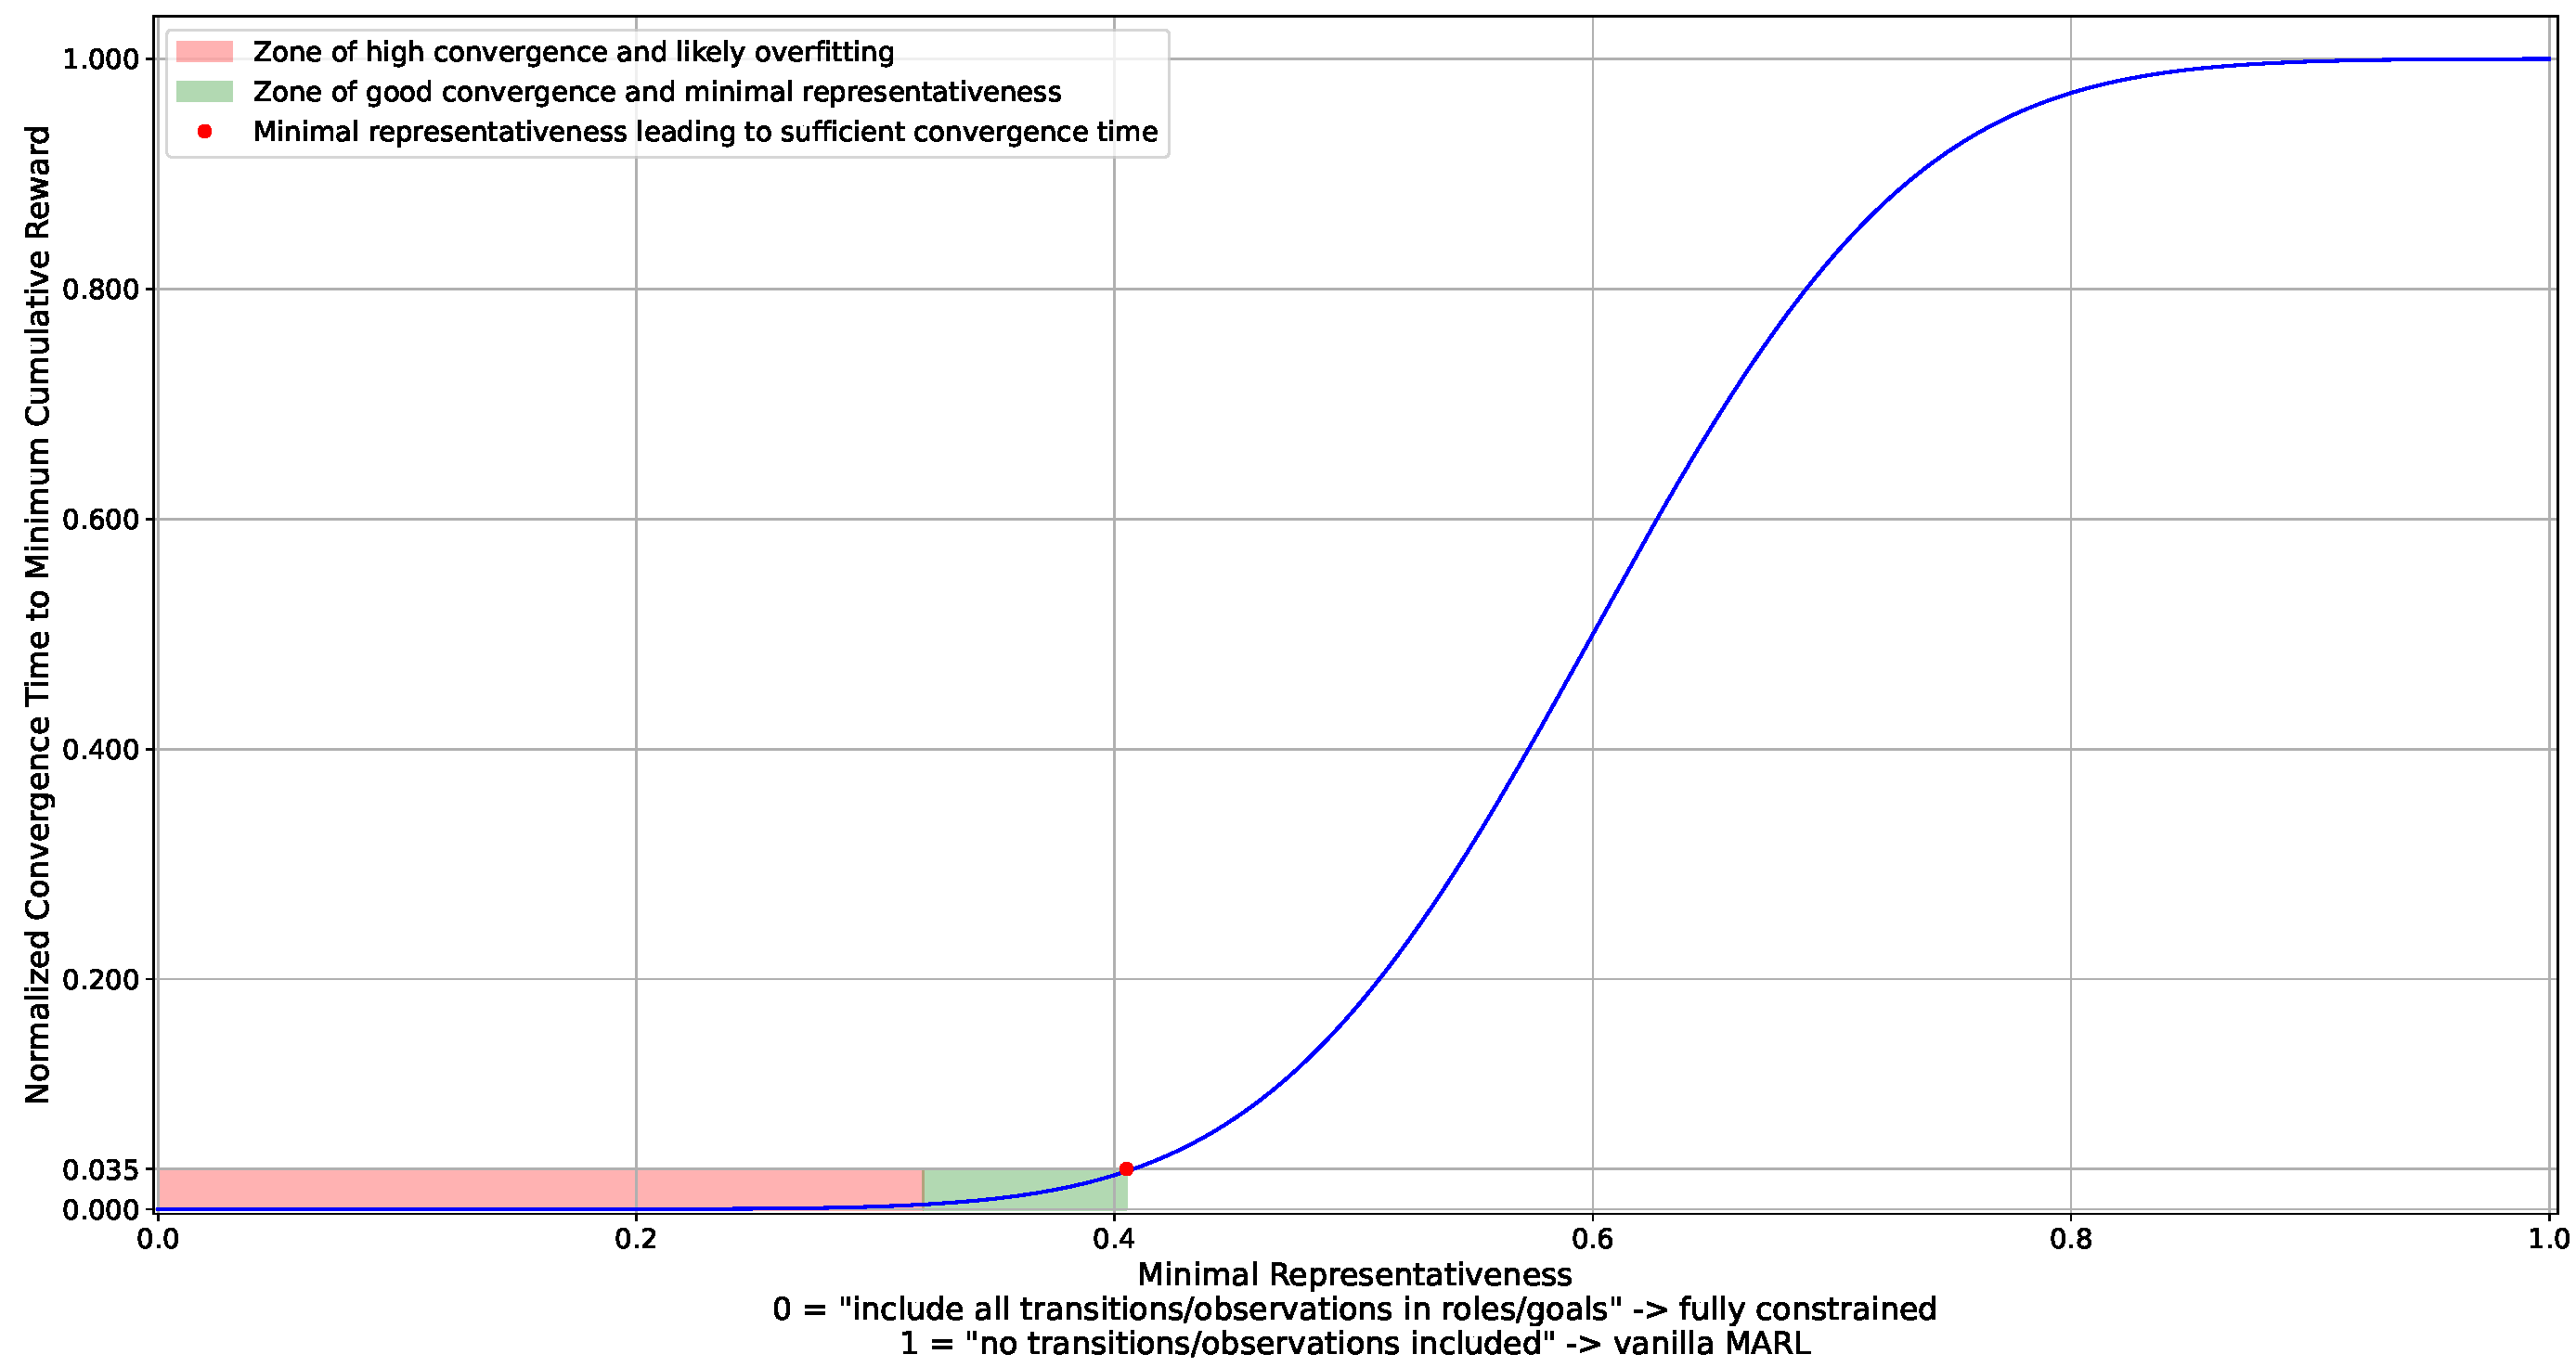
\includegraphics[trim=0cm 0cm 0cm 0cm, clip, width=1.\linewidth]{figures/convergence_time_relative_to_representativeness.pdf}
    \caption{Temps de convergence normalisé en fonction de la représentativité minimale}
    \label{fig:conv_time_repr}
\end{figure}




\section{Description et mise en oeuvre dans l'activité}

L’algorithme~\ref{alg:auto_temm} formalise le déroulement général de l’activité d’analyse.
Chaque étape est détaillée ci-dessous afin d’expliciter les mécanismes qui permettent d’inférer une spécification organisationnelle implicite et de calculer l’adéquation organisationnelle.

\paragraph{Étape 1 : Collecte des trajectoires.}
La première étape consiste à exécuter la politique conjointe $\pi^j$ dans l’environnement $d_\Omega$ afin de générer des historiques complets de transitions $(\omega, a, \omega')$.
Deux ensembles de données sont extraits :
\begin{itemize}
    \item $\mathcal{D}_{\text{trans}}$ contenant les séquences de transitions $(\omega_t, a_t, \omega_{t+1})$, utilisées pour l’inférence des rôles ;
    \item $\mathcal{D}_{\text{obs}}$ contenant uniquement les séquences d’observations $(\omega_t)$, utilisées pour l’inférence des objectifs et missions.
\end{itemize}

\paragraph{Étape 2 : Optimisation des distances et seuils de clustering.}
Pour réduire la variabilité entre trajectoires et identifier des structures récurrentes, les ensembles $\mathcal{D}_{\text{obs}}$ et $\mathcal{D}_{\text{trans}}$ sont soumis à un processus de clustering.
On explore plusieurs métriques de distance $\delta_t$ (ex. \acn{LCS}, Smith-Waterman, distances vectorielles) et seuils de regroupement $\tau_t$.
Chaque combinaison $(\delta_t, \tau_t)$ est évaluée selon un score pondérant :
\[
    \text{Score} = \alpha (\sigma_{\text{obs}} + \sigma_{\text{trans}}) + \beta N_{\text{clusters}}
\]
où $\sigma$ désigne la variance intra-cluster et $N_{\text{clusters}}$ le nombre total de clusters.
La combinaison minimisant ce score est retenue, garantissant un compromis entre cohérence interne et compacité des clusters.

\paragraph{Étape 3 : Application du clustering optimal.}
Une fois les hyperparamètres optimaux $(\delta^*, \tau^*)$ déterminés, les trajectoires sont regroupées :
\begin{itemize}
    \item les clusters de transitions $C_{trans}$ permettent d’inférer les \textbf{rôles} par extraction des séquences communes (\acn{CLS}) et des règles comportementales associées ;
    \item les clusters d’observations $C_{obs}$ servent à identifier les \textbf{objectifs intermédiaires} et les plans associés.
\end{itemize}

\paragraph{Étape 4 : Recherche de représentativité optimale.}
Le degré de représentativité $\rho_t$ fixe le seuil minimal pour qu’une transition ou observation soit retenue comme caractéristique d’un rôle ou objectif.
Une recherche par grille est effectuée sur différentes valeurs de $\rho_t$.
Pour chaque $\rho_t$, une spécification $\mathcal{MM}_{\rho_t}$ est inférée, puis une nouvelle politique $\pi^j_{\rho_t}$ est réentraînée dans $d_\Omega$.
On enregistre alors le temps de convergence $c_{\rho_t}$ pour atteindre une performance minimale $R_{\min}$.
Le paramètre optimal $\rho_t^*$ est choisi comme la plus grande représentativité garantissant une convergence inférieure au seuil $\eta$ (par défaut 3.5\%).

\paragraph{Étape 5 : Inférence finale des rôles et objectifs.}
Avec $(\delta^*, \tau^*, \rho^*)$, on extrait les rôles $\mathcal{R}$, les objectifs intermédiaires $\mathcal{G}$ et leurs relations hiérarchiques (missions, héritage de rôles).
Les permissions et obligations sont déduites en observant la systématicité (obligations) ou la variabilité (permissions) des associations rôle–mission dans les trajectoires.

\paragraph{Étape 6 : Calcul de l’adéquation organisationnelle.}
Deux indicateurs partiels sont calculés :
\begin{itemize}
    \item le \textbf{\acn{SOF}} (structural organizational fit), mesurant la cohérence des rôles via la variance des transitions intra-cluster ;
    \item le \textbf{\acn{FOF}} (functional organizational fit), mesurant la cohérence fonctionnelle dans l’atteinte des objectifs intermédiaires.
\end{itemize}
L’indicateur global est obtenu par agrégation :
\[
    \text{OF} = \frac{1}{2}(\text{SOF} + \text{FOF})
\]

\paragraph{Étape 7 : Sorties de l’activité.}
L’activité retourne :
\begin{itemize}
    \item une spécification implicite $\mathcal{MM}_{\text{implicit}}$ décrivant rôles, missions, permissions et obligations inférés automatiquement ;
    \item un score d’adéquation organisationnelle $\text{OF}$ permettant de quantifier la qualité organisationnelle des comportements émergents.
\end{itemize}


\begin{algorithm}[H]
    \caption{Algorithme de l'activité d'analyse}
    \label{alg:auto_temm}
    \DontPrintSemicolon

    \KwIn{
        Politique conjointe entraînée $\pi^j$~;
        \acn{ODec-POMDP} $d_\Omega$~;
        Spécification initiale $\mathcal{MM}$~;
        Seuil de convergence normalisé (défaut~: 3.5\%) $\eta$
    }

    \KwOut{
    Spécification organisationnelle inférée $\mathcal{MM}_{\text{implicit}}$~;
    Score de adéquation  organisationnel $\acn{OF}$
    }

    \tcp*[l]{1. Collecte des trajectoires}
    Générer les historiques individuels $\mathcal{D}_{\text{trans}}$ depuis $d_\Omega$ sous $\pi^j$ \;
    $\mathcal{D}_{\text{obs}} \gets$ trajectoires d'observations individuelles issues de $\mathcal{D}_{\text{full}}$ \;

    \tcp*[l]{2. \acn{HPO} sur distance et seuil de clustering}
    \For{$t \in \{obs, trans\}$}{
        \ForEach{métrique de distance $\delta_t$}{
            \ForEach{seuil minimal de cluster $\tau_t$}{
                Appliquer clustering avec $(\delta_t, \tau_t)$ \;
                Calculer $\sigma_{\text{obs}}, \sigma_{\text{trans}}, N_{\text{clusters}}$ \;
                Score $\gets \alpha (\sigma_{\text{obs}} + \sigma_{\text{trans}}) + \beta N_{\text{clusters}}$ \tcp*[l]{par défaut~: $\alpha=0.4$, $\beta=0.6$}
                Retenir $(\delta_t^*, \tau_t^*)$ avec Score minimal \;
            }
        }
    }

    \tcp*[l]{3. Application du clustering avec \acn{HPO} optimal}
    Clustering des observations~: $\mathcal{D}_{\text{obs}} \rightarrow C_{obs}$ via $(\delta_{obs}^*, \tau_{obs}^*)$ \;
    Clustering des transitions~: $\mathcal{D}_{\text{trans}} \rightarrow C_{trans}$ via $(\delta_{trans}^*, \tau_{trans}^*)$ \;

    \tcp*[l]{4. \acn{HPO} sur la représentativité (convergence)}
    \For{$t \in \{obs, trans\}$}{
    \ForEach{représentativité $\rho_t$}{
    Inférer $\mathcal{MM}_{\rho_t}$ à partir des clusters \;
    Initialiser une politique $\pi^j_{\rho_t}$ \;
    Entraîner $\pi^j_{\rho_t}$ sur $(d_\Omega, \mathcal{MM}_{\rho_t})$ jusqu'à atteindre $R_{\min}$ \;
    Enregistrer le temps de convergence $c_{\rho_t}$ tel que $ct_t(\rho_t) = c_{\rho_t}$ \;
    }

    \tcp*[l]{5. Sélectionner le point de coude}
    $\rho_t^* \gets max(\{\rho_t \ | \ ct_t(\rho_t) < \eta \})$ \tcp*[r]{par défaut $\eta = 3.5\%$}
    }

    \tcp*[l]{6. Inférence finale des rôles et objectifs}
    Inférer les rôles à partir de $\mathcal{D}_{\text{trans}}, \delta^*, \tau^*, \rho^*$ \;
    Inférer les objectifs à partir de $\mathcal{D}_{\text{obs}}, \delta^*, \tau^*, \rho^*$ \;

    \tcp*[l]{7. Calcul du adéquation  organisationnel}
    Calculer \acn{SOF} et \acn{FOF} à partir des variances intra-cluster \;
    $\text{OF} \gets \frac{1}{2}(\text{SOF} + \text{FOF})$ \;

    \Return{$\mathcal{MM}_{\text{implicit}}, \text{OF}$}
\end{algorithm}


\section{Synthèse, limites et transition}

En synthèse, l’activité d’analyse permet d’établir un lien objectif entre les comportements émergents des agents et les structures organisationnelles attendues. Grâce à la méthode \acn{TEMM} et à son extension Auto-\acn{TEMM}, il devient possible d’inférer automatiquement des rôles, objectifs et missions à partir des trajectoires, et de quantifier leur adéquation organisationnelle par un indicateur robuste. Cette démarche favorise l’explicabilité, la traçabilité et le raffinement itératif des spécifications organisationnelles, tout en fournissant des outils d’évaluation pour comparer différentes politiques ou configurations. Toutefois, la qualité de l’analyse dépend de la diversité des trajectoires collectées et du choix des hyperparamètres de clustering, même si l’automatisation par optimisation conjointe permet de limiter l’intervention humaine. Cette activité constitue ainsi un pivot essentiel pour la boucle de conception \acn{MAMAD}, en préparant le transfert et l’amélioration continue des politiques dans l’environnement réel.


\clearpage
\thispagestyle{empty}
\null
\newpage

\chapter{Transférer et superviser en environnement réel}
\label{chap:transferring}

L'\textit{activité de transfert} correspond à la mise en production et au suivi des politiques conjointes dans l’environnement réel.
Elle joue un double rôle : (i) assurer l’exécution continue de la politique la plus récente $\pi^j_{\text{latest}}$ dans $\mathcal{E}$, garantissant l’action efficace des agents, et (ii) collecter de nouvelles trajectoires réelles $(\omega^j_t, a^j_t, \omega^j_{t+1})$ pour enrichir la base de données $\mathcal{D}_{H^j}$, permettant la mise à jour du modèle simulé et des spécifications organisationnelles.

\section*{Objectifs formels}

Les \textbf{entrées} de l’activité de transfert sont :
\begin{itemize}
    \item la politique conjointe la plus récente $\pi^j_{\text{latest}}$ ;
    \item l’environnement réel $\mathcal{E}$ ;
    \item la base de trajectoires accumulées $\mathcal{D}_{H^j}$.
\end{itemize}

Les \textbf{sorties attendues} sont :
\begin{itemize}
    \item une base enrichie de trajectoires $\mathcal{D}_{H^j}$ ;
    \item un signal $\texttt{need\_update}$ déclenchant la reprise du cycle de conception.
\end{itemize}

La relation globale peut être exprimée par :
\[
    \mathcal{D}_{H^j}, \texttt{need\_update} \gets \texttt{transfer}(\pi^j_{\text{latest}}, \mathcal{E}, \mathcal{D}_{H^j})
\]

\section{Travaux mobilisés et verrous identifiés}

L’activité de transfert et de supervision en environnement réel s’appuie sur plusieurs axes : le transfert de politiques (policy transfer), l’adaptation de domaine (sim2real), la calibration dynamique des modèles (online model calibration), et la supervision continue des systèmes multi-agents.

Les approches de \textit{Robust Reinforcement Learning}~\cite{pinto2017robust} visent à rendre les politiques résistantes aux écarts simulation/réalité, mais n’intègrent pas la mise à jour du modèle simulé après déploiement. Les méthodes d’adaptation de domaine et \textit{Sim2Real}~\cite{tobin2017domain,ganin2016domain} réduisent l’écart simulation/réel via la randomisation ou l’apprentissage de représentations invariantes, mais leur adaptation en ligne reste limitée. Les techniques de calibration dynamique~\cite{deisenroth2011pilco} mettent à jour le modèle simulé à partir des retours du réel, sans prise en compte explicite de l’adaptation des politiques multi-agents. Enfin, la synchronisation manuelle reste courante mais peu adaptée aux environnements dynamiques.

Les principaux verrous sont :
\begin{itemize}
    \item l’absence de cadre unifié pour la mise à jour conjointe du modèle simulé et des politiques déployées ;
    \item la difficulté à détecter et corriger automatiquement les écarts simulation/réalité ;
    \item le manque de mécanismes intégrés pour garantir robustesse et sécurité lors du transfert ;
    \item la nécessité d’une supervision continue et automatisée.
\end{itemize}

Ces limites motivent le développement d’un cadre méthodologique assurant l’adaptation conjointe du jumeau numérique et des politiques multi-agents, avec supervision automatisée du transfert.

\section{Positionnement et contributions proposées}

L’approche proposée introduit un \textbf{cadre de transfert asynchrone et événementiel} comprenant :
\begin{itemize}
    \item une \textbf{Boucle de transfert} (\texttt{Transfer Loop}) qui assure l’exécution en continu de la politique et la collecte des trajectoires dans un tampon temporaire $\mathcal{B}$ ;
    \item un \textbf{Déclencheur de mise à jour} (\texttt{Update Trigger}) qui ajoute les trajectoires à la base $\mathcal{D}_{H^j}$ et active, de façon asynchrone, les activités de modélisation et d’entraînement dès qu’un seuil $\texttt{batch\_size}$ est atteint.
\end{itemize}

Ce double mécanisme assure la continuité du fonctionnement des agents, tout en maintenant la boucle de conception synchronisée avec les données réelles.

\section{Description et mise en œuvre de l’activité}

L’algorithme~\ref{alg:transferring} formalise le fonctionnement de l’activité de transfert.
Chaque élément est décrit ci-dessous afin de préciser les mécanismes et leur rôle dans la boucle de conception.

\paragraph{Entrées et sorties.}
L’activité reçoit en entrée :
\begin{itemize}
    \item la politique conjointe la plus récente $\pi^j_{\text{latest}}$, produite lors de l’entraînement ;
    \item l’environnement réel $\mathcal{E}$, représentant le domaine opérationnel où le \acn{SMA} agit ;
    \item la base courante de trajectoires $\mathcal{D}_{H^j}$, enrichie au fil des déploiements.
\end{itemize}
En sortie, elle retourne :
\begin{itemize}
    \item une base de trajectoires mise à jour $\mathcal{D}_{H^j}$ ;
    \item un signal booléen $\texttt{need\_update}$ indiquant si les activités de modélisation et d’entraînement doivent être relancées.
\end{itemize}

\paragraph{Boucle de transfert.}
La boucle de transfert s’exécute tant que le \acn{SMA} est actif dans $\mathcal{E}$.
À chaque pas de temps $t$ :
\begin{enumerate}
    \item une observation $\omega^j_t$ est collectée via la fonction $\texttt{observe}(\mathcal{E})$ ;
    \item l’action $a^j_t$ est choisie en appliquant la politique $\pi^j_{\text{latest}}$ à l’observation courante ;
    \item cette action est exécutée dans l’environnement via $\texttt{apply}(\mathcal{E}, a^j_t)$, produisant la nouvelle observation $\omega^j_{t+1}$ ;
    \item la transition $(\omega^j_t, a^j_t, \omega^j_{t+1})$ est stockée dans un tampon temporaire $\mathcal{B}$.
\end{enumerate}

\paragraph{Déclencheur de mise à jour.}
Lorsque la taille du tampon $\mathcal{B}$ dépasse un seuil $\texttt{batch\_size}$, le contenu est ajouté à la base de trajectoires $\mathcal{D}_{H^j}$ puis le tampon est vidé.
Le signal $\texttt{need\_update}$ est alors activé.
Si aucun processus de mise à jour n’est en cours (\texttt{not running\_update}), la procédure \texttt{launch\_update()} est déclenchée de manière asynchrone pour relancer les activités de modélisation et d’entraînement.

\paragraph{Fonctionnement global.}
Ce schéma assure trois propriétés essentielles :
\begin{itemize}
    \item la \textbf{continuité d’exécution} : les agents opèrent toujours avec la dernière politique disponible ;
    \item la \textbf{réactivité} : les données réelles sont intégrées dès qu’un volume suffisant est collecté ;
    \item la \textbf{automatisation} : les mises à jour se déclenchent sans intervention humaine, tout en évitant les conflits entre processus parallèles.
\end{itemize}

\paragraph{Éléments formels.}
Ainsi, l’algorithme encode la relation :
\[
    \mathcal{D}_{H^j}, \texttt{need\_update} \gets \texttt{transfer}(\pi^j_{\text{latest}}, \mathcal{E}, \mathcal{D}_{H^j})
\]
où :
\begin{itemize}
    \item $\mathcal{B}$ désigne le tampon temporaire,
    \item $\texttt{batch\_size}$ fixe la granularité de déclenchement des mises à jour,
    \item $\texttt{launch\_update}()$ assure la synchronisation avec les autres activités de la méthode \acn{MAMAD}.
\end{itemize}

\vspace{-0.3em}
\begin{algorithm}[H]
    \caption{Activité de transfert}
    \label{alg:transferring}
    \DontPrintSemicolon
    \KwIn{Politique actuelle $\pi^j_{\text{latest}}$, environnement réel $\mathcal{E}$, base de trajectoires $\mathcal{D}_{H^j}$}
    \KwOut{Base de trajectoires mise à jour $\mathcal{D}_{H^j}$, signal de mise à jour $\texttt{need\_update}$}

    \vspace{0.3em}
    \SetKwProg{Transfer}{Procédure \normalfont BoucleDeTransfert}{}{}
    \Transfer{}{

    \While{le \acn{SMA} est actif dans l'environnement $\mathcal{E}$}{
    \tcp*[l]{Exécution de la politique la plus récente}
    $\omega^j_t \gets \texttt{observe}(\mathcal{E})$ \;
    $a^j_t \gets \pi^j_{\text{latest}}(\omega^j_t)$ \;
    $\omega^j_{t+1} \gets \texttt{apply}(\mathcal{E}, a^j_t)$ \;
    Ajouter $(\omega^j_t, a^j_t, \omega^j_{t+1})$ au tampon temporaire $\mathcal{B}$ \;

    \tcp*[l]{Vérification du déclenchement de la mise à jour}
    \If{$|\mathcal{B}| \geq \texttt{batch\_size}$}{
        Ajouter $\mathcal{B}$ à $\mathcal{D}_{H^j}$ et vider $\mathcal{B}$ \;
        $\texttt{need\_update} \gets \texttt{True}$ \;
        \If{$\texttt{not running\_update} = \texttt{False}$}{
            \texttt{launch\_update()} \tcp*[r]{Appel asynchrone}
        }
    }
    }
    }
\end{algorithm}


\section{Synthèse, limites et transition}

En synthèse, l’activité de transfert assure l’exécution continue de la politique la plus récente et la collecte automatisée de trajectoires réelles pour raffiner le modèle et réentraîner les politiques.

Ses atouts sont :
\begin{itemize}
    \item automatisation du déploiement et de la collecte en environnement réel ;
    \item synchronisation robuste avec les autres activités de \acn{MAMAD} ;
    \item adaptation continue des agents à l’environnement.
\end{itemize}

Ses limites portent sur le coût de supervision, la gestion des environnements critiques, et la fréquence optimale des mises à jour.

Cette activité permet une méthode réellement \textbf{autoadaptative}, alternant apprentissage simulé et déploiement réel pour garantir la robustesse des \acn{SMA} en contexte dynamique.



\clearpage
\thispagestyle{empty}
\null
\newpage

\chapter*{Conclusion}
\addcontentsline{toc}{chapter}{\textbf{Conclusion}}

\noindent
Cette troisième partie a introduit la méthode \textbf{\acn{MAMAD}} comme une réponse concrète aux limites identifiées dans les approches actuelles de conception de \acn{SMA}. Reposant sur un cycle itératif structuré en quatre activités (\textit{Modélisation}, \textit{Apprentissage}, \textit{Analyse}, \textit{Transfert}), \acn{MAMAD} articule de manière cohérente des outils symboliques (spécifications organisationnelles) et \acn{MARL} pour guider la conception, l'entraînement et l'adaptation d'agents intelligents dans des environnements complexes.

\medskip

\noindent
La méthode s'appuie notamment~:
\begin{itemize}
    \item sur une modélisation fidèle des environnements à partir de données empiriques,
    \item sur un entraînement contraint par des spécifications organisationnelles intégrées au sein du cadre \textit{MOISE+MARL},
    \item sur une analyse des trajectoires pour inférer les structures émergentes de l'organisation apprise,
    \item et enfin sur un transfert contrôlé permettant l'amélioration itérative du \acn{SMA}.
\end{itemize}

\noindent
Dans la partie suivante, nous proposons de valider expérimentalement cette méthode à travers son implémentation concrète dans un outil dédié, \acn{CybMASDE}, et son application à plusieurs environnements représentatifs. L'objectif est de démontrer la capacité de \acn{MAMAD} à produire automatiquement des \acplu{SMA} performants, explicables et conformes à des exigences organisationnelles dans des contextes variés.

\medskip

\noindent
Nous évaluons notamment la méthode selon des critères d'efficacité, d'automatisation, de conformité aux contraintes et d'explicabilité, tout en comparant ses résultats à ceux d'approches classiques non guidées par des modèles organisationnels.

\bigskip

La \autoref{part:experimentation} met donc à l'épreuve la méthode \acn{MAMAD}, en analysant ses performances et sa pertinence au regard des verrous identifiés sur différents scénarios.
